\documentclass[12pt,a4paper]{report}
\usepackage{graphicx,../iman,../extra,../ttbox,../proof,../pdfsetup}

%%\includeonly{}
%%% to index ids: \[\\tt \([a-zA-Z0-9][a-zA-Z0-9_'.]*\)    [\\ttindexbold{\1}
%%% to delete old ones:  \\indexbold{\*[^}]*}
%% run    sedindex ref    to prepare index file
%%% needs chapter on Provers/typedsimp.ML?
\title{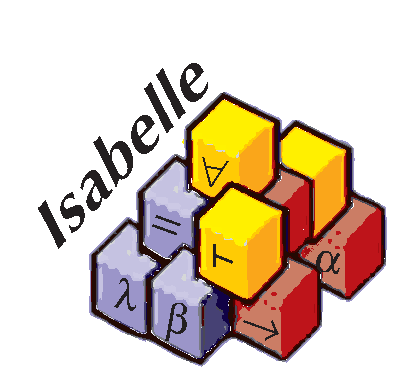
\includegraphics[scale=0.5]{isabelle} \\[4ex] Old Isabelle Reference Manual}

\author{{\em Lawrence C. Paulson}\\
        Computer Laboratory \\ University of Cambridge \\
        \texttt{lcp@cl.cam.ac.uk}\\[3ex] 
        With Contributions by Tobias Nipkow and Markus Wenzel}  

\makeindex

\setcounter{secnumdepth}{2} \setcounter{tocdepth}{2}

\pagestyle{headings}
\sloppy
\binperiod     %%%treat . like a binary operator

\begin{document}
\underscoreoff

\index{definitions|see{rewriting, meta-level}}
\index{rewriting!object-level|see{simplification}}
\index{meta-rules|see{meta-rules}}

\maketitle 
\emph{Note}: this document is part of the earlier Isabelle
documentation and is mostly outdated.  Fully obsolete parts of the
original text have already been removed.  The remaining material
covers some aspects that did not make it into the newer manuals yet.

\subsubsection*{Acknowledgements} 
Tobias Nipkow, of T. U. Munich, wrote most of
  Chapters~\protect\ref{Defining-Logics} and~\protect\ref{chap:simplification}.
  Markus Wenzel contributed to Chapter~\protect\ref{chap:syntax}.
  Jeremy Dawson, Sara Kalvala, Martin
  Simons  and others suggested changes
  and corrections.  The research has been funded by the EPSRC (grants
  GR/G53279, GR/H40570, GR/K57381, GR/K77051, GR/M75440) and by ESPRIT
  (projects 3245: Logical Frameworks, and 6453: Types), and by the DFG
  Schwerpunktprogramm \emph{Deduktion}.

\pagenumbering{roman} \tableofcontents \clearfirst


%% $Id$

\chapter{Basic Use of Isabelle}\index{sessions|(} 
The Reference Manual is a comprehensive description of Isabelle
proper, including all \ML{} commands, functions and packages.  It
really is intended for reference, perhaps for browsing, but not for
reading through.  It is not a tutorial, but assumes familiarity with
the basic logical concepts of Isabelle.

When you are looking for a way of performing some task, scan the Table of
Contents for a relevant heading.  Functions are organized by their purpose,
by their operands (subgoals, tactics, theorems), and by their usefulness.
In each section, basic functions appear first, then advanced functions, and
finally esoteric functions.  Use the Index when you are looking for the
definition of a particular Isabelle function.

A few examples are presented.  Many example files are distributed with
Isabelle, however; please experiment interactively.


\section{Basic interaction with Isabelle}
\index{starting up|bold}\nobreak
%
We assume that your local Isabelle administrator (this might be you!) has
already installed the Isabelle system together with appropriate object-logics
--- otherwise see the \texttt{README} and \texttt{INSTALL} files in the
top-level directory of the distribution on how to do this.

\medskip Let $\langle isabellehome \rangle$ denote the location where
the distribution has been installed.  To run Isabelle from a the shell
prompt within an ordinary text terminal session, simply type
\begin{ttbox}
\({\langle}isabellehome{\rangle}\)/bin/isabelle
\end{ttbox}
This should start an interactive \ML{} session with the default object-logic
(usually {\HOL}) already pre-loaded.

Subsequently, we assume that the \texttt{isabelle} executable is determined
automatically by the shell, e.g.\ by adding {\tt \(\langle isabellehome
  \rangle\)/bin} to your search path.\footnote{Depending on your installation,
  there might be also stand-alone binaries located in some global directory
  such as \texttt{/usr/bin}.  Do not attempt to copy {\tt \(\langle
    isabellehome \rangle\)/bin/isabelle}, though!  See \texttt{isatool
    install} in \emph{The Isabelle System Manual} of how to do this properly.}

\medskip

The object-logic image to load may be also specified explicitly as an argument
to the {\tt isabelle} command, e.g.
\begin{ttbox}
isabelle FOL
\end{ttbox}
This should put you into the world of polymorphic first-order logic (assuming
that an image of {\FOL} has been pre-built).

\index{saving your session|bold} Isabelle provides no means of storing
theorems or internal proof objects on files.  Theorems are simply part of the
\ML{} state.  To save your work between sessions, you may dump the \ML{}
system state to a file.  This is done automatically when ending the session
normally (e.g.\ by typing control-D), provided that the image has been opened
\emph{writable} in the first place.  The standard object-logic images are
usually read-only, so you have to create a private working copy first.  For
example, the following shell command puts you into a writable Isabelle session
of name \texttt{Foo} that initially contains just plain \HOL:
\begin{ttbox}
isabelle HOL Foo
\end{ttbox}
Ending the \texttt{Foo} session with control-D will cause the complete
\ML-world to be saved somewhere in your home directory\footnote{The default
  location is in \texttt{\~\relax/isabelle/heaps}, but this depends on your
  local configuration.}.  Make sure there is enough space available! Then one
may later continue at exactly the same point by running
\begin{ttbox}
isabelle Foo  
\end{ttbox}

\medskip Saving the {\ML} state is not enough.  Record, on a file, the
top-level commands that generate your theories and proofs.  Such a record
allows you to replay the proofs whenever required, for instance after making
minor changes to the axioms.  Ideally, these sources will be somewhat
intelligible to others as a formal description of your work.

It is good practice to put all source files that constitute a separate
Isabelle session into an individual directory, together with an {\ML} file
called \texttt{ROOT.ML} that contains appropriate commands to load all other
files required.  Running \texttt{isabelle} with option \texttt{-u}
automatically loads \texttt{ROOT.ML} on entering the session.  The
\texttt{isatool usedir} utility provides some more options to manage Isabelle
sessions, such as automatic generation of theory browsing information.

\medskip More details about the \texttt{isabelle} and \texttt{isatool}
commands may be found in \emph{The Isabelle System Manual}.

\medskip There are more comfortable user interfaces than the bare-bones \ML{}
top-level run from a text terminal.  The \texttt{Isabelle} executable (note
the capital I) runs one such interface, depending on your local configuration.
Again, see \emph{The Isabelle System Manual} for more information.


\section{Ending a session}
\begin{ttbox} 
quit    : unit -> unit
exit    : int -> unit
commit  : unit -> bool
\end{ttbox}
\begin{ttdescription}
\item[\ttindexbold{quit}();] ends the Isabelle session, without saving
  the state.
  
\item[\ttindexbold{exit} \(i\);] similar to {\tt quit}, passing return
  code \(i\) to the operating system.

\item[\ttindexbold{commit}();] saves the current state without ending
  the session, provided that the logic image is opened read-write;
  return value {\tt false} indicates an error.
\end{ttdescription}

Typing control-D also finishes the session in essentially the same way
as the sequence {\tt commit(); quit();} would.


\section{Reading ML files}
\index{files!reading}
\begin{ttbox} 
cd              : string -> unit
pwd             : unit -> string
use             : string -> unit
time_use        : string -> unit
\end{ttbox}
\begin{ttdescription}
\item[\ttindexbold{cd} "{\it dir}";] changes the current directory to
  {\it dir}.  This is the default directory for reading files.
  
\item[\ttindexbold{pwd}();] returns the full path of the current
  directory.

\item[\ttindexbold{use} "$file$";]  
reads the given {\it file} as input to the \ML{} session.  Reading a file
of Isabelle commands is the usual way of replaying a proof.

\item[\ttindexbold{time_use} "$file$";]  
performs {\tt use~"$file$"} and prints the total execution time.
\end{ttdescription}

The $dir$ and $file$ specifications of the \texttt{cd} and \texttt{use}
commands may contain path variables (e.g.\ \texttt{\$ISABELLE_HOME}) that are
expanded appropriately.  Note that \texttt{\~\relax} abbreviates
\texttt{\$HOME}, and \texttt{\~\relax\~\relax} abbreviates
\texttt{\$ISABELLE_HOME}\index{*\$ISABELLE_HOME}.  The syntax for path
specifications follows Unix conventions.


\section{Reading theories}\label{sec:intro-theories}
\index{theories!reading}

In Isabelle, any kind of declarations, definitions, etc.\ are organized around
named \emph{theory} objects.  Logical reasoning always takes place within a
certain theory context, which may be switched at any time.  Theory $name$ is
defined by a theory file $name$\texttt{.thy}, containing declarations of
\texttt{consts}, \texttt{types}, \texttt{defs}, etc.\ (see
\S\ref{sec:ref-defining-theories} for more details on concrete syntax).
Furthermore, there may be an associated {\ML} file $name$\texttt{.ML} with
proof scripts that are to be run in the context of the theory.

\begin{ttbox}
context      : theory -> unit
the_context  : unit -> theory
theory       : string -> theory
use_thy      : string -> unit
time_use_thy : string -> unit
update_thy   : string -> unit
\end{ttbox}

\begin{ttdescription}
  
\item[\ttindexbold{context} $thy$;] switches the current theory context.  Any
  subsequent command with ``implicit theory argument'' (e.g.\ \texttt{Goal})
  will refer to $thy$ as its theory.
  
\item[\ttindexbold{the_context}();] obtains the current theory context, or
  raises an error if absent.
  
\item[\ttindexbold{theory} "$name$";] retrieves the theory called $name$ from
  the internal database of loaded theories, raising an error if absent.
  
\item[\ttindexbold{use_thy} "$name$";] reads theory $name$ from the file
  system, looking for $name$\texttt{.thy} and $name$\texttt{.ML} (the latter
  being optional).  It also ensures that all parent theories are loaded as
  well.  In case some older versions have already been present,
  \texttt{use_thy} only tries to reload $name$ itself, but is content with any
  version of its ancestors.
  
\item[\ttindexbold{time_use_thy} "$name$";] same as \texttt{use_thy}, but
  reports the time taken to process the actual theory parts and {\ML} files
  separately.

\item[\ttindexbold{update_thy} "$name$";] is similar to \texttt{use_thy}, but
  ensures that theory $name$ is fully up-to-date with respect to the file
  system --- apart from $name$ itself any of its ancestors may be reloaded as
  well.
  
\end{ttdescription}

Note that theories of pre-built logic images (e.g.\ {\HOL}) are marked as
\emph{finished} and cannot be updated any more.  See \S\ref{sec:more-theories}
for further information on Isabelle's theory loader.


\section{Setting flags}
\begin{ttbox}
set     : bool ref -> bool
reset   : bool ref -> bool
toggle  : bool ref -> bool
\end{ttbox}\index{*set}\index{*reset}\index{*toggle}
These are some shorthands for manipulating boolean references.  The new
value is returned.


\section{Printing of terms and theorems}\label{sec:printing-control}
\index{printing control|(}
Isabelle's pretty printer is controlled by a number of parameters.

\subsection{Printing limits}
\begin{ttbox} 
Pretty.setdepth  : int -> unit
Pretty.setmargin : int -> unit
print_depth      : int -> unit
\end{ttbox}
These set limits for terminal output.  See also {\tt goals_limit},
which limits the number of subgoals printed
(\S\ref{sec:goals-printing}).

\begin{ttdescription}
\item[\ttindexbold{Pretty.setdepth} \(d\);] tells Isabelle's pretty printer to
  limit the printing depth to~$d$.  This affects the display of theorems and
  terms.  The default value is~0, which permits printing to an arbitrary
  depth.  Useful values for $d$ are~10 and~20.

\item[\ttindexbold{Pretty.setmargin} \(m\);]  
  tells Isabelle's pretty printer to assume a right margin (page width)
  of~$m$.  The initial margin is~76.

\item[\ttindexbold{print_depth} \(n\);]  
  limits the printing depth of complex \ML{} values, such as theorems and
  terms.  This command affects the \ML{} top level and its effect is
  compiler-dependent.  Typically $n$ should be less than~10.
\end{ttdescription}


\subsection{Printing of hypotheses, brackets, types etc.}
\index{meta-assumptions!printing of}
\index{types!printing of}\index{sorts!printing of}
\begin{ttbox} 
show_hyps     : bool ref \hfill{\bf initially true}
show_tags     : bool ref \hfill{\bf initially false}
show_brackets : bool ref \hfill{\bf initially false}
show_types    : bool ref \hfill{\bf initially false}
show_sorts    : bool ref \hfill{\bf initially false}
show_consts   : bool ref \hfill{\bf initially false}
long_names    : bool ref \hfill{\bf initially false}
\end{ttbox}
These flags allow you to control how much information is displayed for
types, terms and theorems.  The hypotheses of theorems \emph{are}
normally shown.  Superfluous parentheses of types and terms are not.
Types and sorts of variables are normally hidden.

Note that displaying types and sorts may explain why a polymorphic
inference rule fails to resolve with some goal, or why a rewrite rule
does not apply as expected.

\begin{ttdescription}

\item[reset \ttindexbold{show_hyps};] makes Isabelle show each
  meta-level hypothesis as a dot.
  
\item[set \ttindexbold{show_tags};] makes Isabelle show tags of theorems
  (which are basically just comments that may be attached by some tools).
  
\item[set \ttindexbold{show_brackets};] makes Isabelle show full
  bracketing.  In particular, this reveals the grouping of infix
  operators.
  
\item[set \ttindexbold{show_types};] makes Isabelle show types when
  printing a term or theorem.
  
\item[set \ttindexbold{show_sorts};] makes Isabelle show both types
  and the sorts of type variables, independently of the value of
  \texttt{show_types}.

\item[set \ttindexbold{show_consts};] makes Isabelle show types of
  constants, provided that showing of types is enabled at all.  This
  is supported for printing of proof states only.  Note that the
  output can be enormous as polymorphic constants often occur at
  several different type instances.

\item[set \ttindexbold{long_names};] forces names of all objects
  (types, constants, theorems, etc.) to be printed in their fully
  qualified internal form.

\end{ttdescription}


\subsection{Eta-contraction before printing}
\begin{ttbox} 
eta_contract: bool ref \hfill{\bf initially false}
\end{ttbox}
The {\bf $\eta$-contraction law} asserts $(\lambda x.f(x))\equiv f$,
provided $x$ is not free in ~$f$.  It asserts {\bf extensionality} of
functions: $f\equiv g$ if $f(x)\equiv g(x)$ for all~$x$.  Higher-order
unification frequently puts terms into a fully $\eta$-expanded form.  For
example, if $F$ has type $(\tau\To\tau)\To\tau$ then its expanded form is
$\lambda h.F(\lambda x.h(x))$.  By default, the user sees this expanded
form.

\begin{ttdescription}
\item[set \ttindexbold{eta_contract};]
makes Isabelle perform $\eta$-contractions before printing, so that
$\lambda h.F(\lambda x.h(x))$ appears simply as~$F$.  The
distinction between a term and its $\eta$-expanded form occasionally
matters.
\end{ttdescription}
\index{printing control|)}

\section{Diagnostic messages}
\index{error messages}
\index{warnings}

Isabelle conceptually provides three output channels for different kinds of
messages: ordinary text, warnings, errors.  Depending on the user interface
involved, these messages may appear in different text styles or colours.

The default setup of an \texttt{isabelle} terminal session is as
follows: plain output of ordinary text, warnings prefixed by
\texttt{\#\#\#}'s, errors prefixed by \texttt{***}'s.  For example, a
typical warning would look like this:
\begin{ttbox}
\#\#\# Beware the Jabberwock, my son!
\#\#\# The jaws that bite, the claws that catch!
\#\#\# Beware the Jubjub Bird, and shun
\#\#\# The frumious Bandersnatch!
\end{ttbox}

\texttt{ML} programs may output diagnostic messages using the
following functions:
\begin{ttbox}
writeln : string -> unit
warning : string -> unit
error   : string -> 'a
\end{ttbox}
Note that \ttindex{error} fails by raising exception \ttindex{ERROR}
after having output the text, while \ttindex{writeln} and
\ttindex{warning} resume normal program execution.


\section{Displaying exceptions as error messages}
\index{exceptions!printing of}
\begin{ttbox} 
print_exn: exn -> 'a
\end{ttbox}
Certain Isabelle primitives, such as the forward proof functions {\tt RS}
and {\tt RSN}, are called both interactively and from programs.  They
indicate errors not by printing messages, but by raising exceptions.  For
interactive use, \ML's reporting of an uncaught exception may be
uninformative.  The Poly/ML function {\tt exception_trace} can generate a
backtrace.\index{Poly/{\ML} compiler}

\begin{ttdescription}
\item[\ttindexbold{print_exn} $e$] 
displays the exception~$e$ in a readable manner, and then re-raises~$e$.
Typical usage is~\hbox{\tt $EXP$ handle e => print_exn e;}, where
$EXP$ is an expression that may raise an exception.

{\tt print_exn} can display the following common exceptions, which concern
types, terms, theorems and theories, respectively.  Each carries a message
and related information.
\begin{ttbox} 
exception TYPE   of string * typ list * term list
exception TERM   of string * term list
exception THM    of string * int * thm list
exception THEORY of string * theory list
\end{ttbox}
\end{ttdescription}
\begin{warn}
  {\tt print_exn} prints terms by calling \ttindex{prin}, which obtains
  pretty printing information from the proof state last stored in the
  subgoal module.  The appearance of the output thus depends upon the
  theory used in the last interactive proof.
\end{warn}

\index{sessions|)}


%%% Local Variables: 
%%% mode: latex
%%% TeX-master: "ref"
%%% End: 

%% $Id$
\chapter{Tactics} \label{tactics}
\index{tactics|(} Tactics have type \mltydx{tactic}.  This is just an
abbreviation for functions from theorems to theorem sequences, where
the theorems represent states of a backward proof.  Tactics seldom
need to be coded from scratch, as functions; instead they are
expressed using basic tactics and tacticals.

This chapter only presents the primitive tactics.  Substantial proofs
require the power of automatic tools like simplification
(Chapter~\ref{chap:simplification}) and classical tableau reasoning
(Chapter~\ref{chap:classical}).

\section{Resolution and assumption tactics}
{\bf Resolution} is Isabelle's basic mechanism for refining a subgoal using
a rule.  {\bf Elim-resolution} is particularly suited for elimination
rules, while {\bf destruct-resolution} is particularly suited for
destruction rules.  The {\tt r}, {\tt e}, {\tt d} naming convention is
maintained for several different kinds of resolution tactics, as well as
the shortcuts in the subgoal module.

All the tactics in this section act on a subgoal designated by a positive
integer~$i$.  They fail (by returning the empty sequence) if~$i$ is out of
range.

\subsection{Resolution tactics}
\index{resolution!tactics}
\index{tactics!resolution|bold}
\begin{ttbox} 
resolve_tac  : thm list -> int -> tactic
eresolve_tac : thm list -> int -> tactic
dresolve_tac : thm list -> int -> tactic
forward_tac  : thm list -> int -> tactic 
\end{ttbox}
These perform resolution on a list of theorems, $thms$, representing a list
of object-rules.  When generating next states, they take each of the rules
in the order given.  Each rule may yield several next states, or none:
higher-order resolution may yield multiple resolvents.
\begin{ttdescription}
\item[\ttindexbold{resolve_tac} {\it thms} {\it i}] 
  refines the proof state using the rules, which should normally be
  introduction rules.  It resolves a rule's conclusion with
  subgoal~$i$ of the proof state.

\item[\ttindexbold{eresolve_tac} {\it thms} {\it i}] 
  \index{elim-resolution}
  performs elim-resolution with the rules, which should normally be
  elimination rules.  It resolves with a rule, proves its first premise by
  assumption, and finally \emph{deletes} that assumption from any new
  subgoals.  (To rotate a rule's premises,
  see \texttt{rotate_prems} in~\S\ref{MiscellaneousForwardRules}.)

\item[\ttindexbold{dresolve_tac} {\it thms} {\it i}] 
  \index{forward proof}\index{destruct-resolution}
  performs destruct-resolution with the rules, which normally should
  be destruction rules.  This replaces an assumption by the result of
  applying one of the rules.

\item[\ttindexbold{forward_tac}]\index{forward proof}
  is like {\tt dresolve_tac} except that the selected assumption is not
  deleted.  It applies a rule to an assumption, adding the result as a new
  assumption.
\end{ttdescription}

\subsection{Assumption tactics}
\index{tactics!assumption|bold}\index{assumptions!tactics for}
\begin{ttbox} 
assume_tac    : int -> tactic
eq_assume_tac : int -> tactic
\end{ttbox} 
\begin{ttdescription}
\item[\ttindexbold{assume_tac} {\it i}] 
attempts to solve subgoal~$i$ by assumption.

\item[\ttindexbold{eq_assume_tac}] 
is like {\tt assume_tac} but does not use unification.  It succeeds (with a
\emph{unique} next state) if one of the assumptions is identical to the
subgoal's conclusion.  Since it does not instantiate variables, it cannot
make other subgoals unprovable.  It is intended to be called from proof
strategies, not interactively.
\end{ttdescription}

\subsection{Matching tactics} \label{match_tac}
\index{tactics!matching}
\begin{ttbox} 
match_tac  : thm list -> int -> tactic
ematch_tac : thm list -> int -> tactic
dmatch_tac : thm list -> int -> tactic
\end{ttbox}
These are just like the resolution tactics except that they never
instantiate unknowns in the proof state.  Flexible subgoals are not updated
willy-nilly, but are left alone.  Matching --- strictly speaking --- means
treating the unknowns in the proof state as constants; these tactics merely
discard unifiers that would update the proof state.
\begin{ttdescription}
\item[\ttindexbold{match_tac} {\it thms} {\it i}] 
refines the proof state using the rules, matching a rule's
conclusion with subgoal~$i$ of the proof state.

\item[\ttindexbold{ematch_tac}] 
is like {\tt match_tac}, but performs elim-resolution.

\item[\ttindexbold{dmatch_tac}] 
is like {\tt match_tac}, but performs destruct-resolution.
\end{ttdescription}


\subsection{Resolution with instantiation} \label{res_inst_tac}
\index{tactics!instantiation}\index{instantiation}
\begin{ttbox} 
res_inst_tac  : (string*string)list -> thm -> int -> tactic
eres_inst_tac : (string*string)list -> thm -> int -> tactic
dres_inst_tac : (string*string)list -> thm -> int -> tactic
forw_inst_tac : (string*string)list -> thm -> int -> tactic
\end{ttbox}
These tactics are designed for applying rules such as substitution and
induction, which cause difficulties for higher-order unification.  The
tactics accept explicit instantiations for unknowns in the rule ---
typically, in the rule's conclusion.  Each instantiation is a pair
{\tt($v$,$e$)}, where $v$ is an unknown \emph{without} its leading
question mark!
\begin{itemize}
\item If $v$ is the type unknown {\tt'a}, then
the rule must contain a type unknown \verb$?'a$ of some
sort~$s$, and $e$ should be a type of sort $s$.

\item If $v$ is the unknown {\tt P}, then
the rule must contain an unknown \verb$?P$ of some type~$\tau$,
and $e$ should be a term of some type~$\sigma$ such that $\tau$ and
$\sigma$ are unifiable.  If the unification of $\tau$ and $\sigma$
instantiates any type unknowns in $\tau$, these instantiations
are recorded for application to the rule.
\end{itemize}
Types are instantiated before terms.  Because type instantiations are
inferred from term instantiations, explicit type instantiations are seldom
necessary --- if \verb$?t$ has type \verb$?'a$, then the instantiation list
\verb$[("'a","bool"),("t","True")]$ may be simplified to
\verb$[("t","True")]$.  Type unknowns in the proof state may cause
failure because the tactics cannot instantiate them.

The instantiation tactics act on a given subgoal.  Terms in the
instantiations are type-checked in the context of that subgoal --- in
particular, they may refer to that subgoal's parameters.  Any unknowns in
the terms receive subscripts and are lifted over the parameters; thus, you
may not refer to unknowns in the subgoal.

\begin{ttdescription}
\item[\ttindexbold{res_inst_tac} {\it insts} {\it thm} {\it i}]
instantiates the rule {\it thm} with the instantiations {\it insts}, as
described above, and then performs resolution on subgoal~$i$.  Resolution
typically causes further instantiations; you need not give explicit
instantiations for every unknown in the rule.

\item[\ttindexbold{eres_inst_tac}] 
is like {\tt res_inst_tac}, but performs elim-resolution.

\item[\ttindexbold{dres_inst_tac}] 
is like {\tt res_inst_tac}, but performs destruct-resolution.

\item[\ttindexbold{forw_inst_tac}] 
is like {\tt dres_inst_tac} except that the selected assumption is not
deleted.  It applies the instantiated rule to an assumption, adding the
result as a new assumption.
\end{ttdescription}


\section{Other basic tactics}
\subsection{Tactic shortcuts}
\index{shortcuts!for tactics}
\index{tactics!resolution}\index{tactics!assumption}
\index{tactics!meta-rewriting}
\begin{ttbox} 
rtac     :      thm -> int -> tactic
etac     :      thm -> int -> tactic
dtac     :      thm -> int -> tactic
atac     :             int -> tactic
ares_tac : thm list -> int -> tactic
rewtac   :      thm ->        tactic
\end{ttbox}
These abbreviate common uses of tactics.
\begin{ttdescription}
\item[\ttindexbold{rtac} {\it thm} {\it i}] 
abbreviates \hbox{\tt resolve_tac [{\it thm}] {\it i}}, doing resolution.

\item[\ttindexbold{etac} {\it thm} {\it i}] 
abbreviates \hbox{\tt eresolve_tac [{\it thm}] {\it i}}, doing elim-resolution.

\item[\ttindexbold{dtac} {\it thm} {\it i}] 
abbreviates \hbox{\tt dresolve_tac [{\it thm}] {\it i}}, doing
destruct-resolution.

\item[\ttindexbold{atac} {\it i}] 
abbreviates \hbox{\tt assume_tac {\it i}}, doing proof by assumption.

\item[\ttindexbold{ares_tac} {\it thms} {\it i}] 
tries proof by assumption and resolution; it abbreviates
\begin{ttbox}
assume_tac {\it i} ORELSE resolve_tac {\it thms} {\it i}
\end{ttbox}

\item[\ttindexbold{rewtac} {\it def}] 
abbreviates \hbox{\tt rewrite_goals_tac [{\it def}]}, unfolding a definition.
\end{ttdescription}


\subsection{Inserting premises and facts}\label{cut_facts_tac}
\index{tactics!for inserting facts}\index{assumptions!inserting}
\begin{ttbox} 
cut_facts_tac : thm list -> int -> tactic
cut_inst_tac  : (string*string)list -> thm -> int -> tactic
subgoal_tac   : string -> int -> tactic
subgoal_tacs  : string list -> int -> tactic
\end{ttbox}
These tactics add assumptions to a subgoal.
\begin{ttdescription}
\item[\ttindexbold{cut_facts_tac} {\it thms} {\it i}] 
  adds the {\it thms} as new assumptions to subgoal~$i$.  Once they have
  been inserted as assumptions, they become subject to tactics such as {\tt
    eresolve_tac} and {\tt rewrite_goals_tac}.  Only rules with no premises
  are inserted: Isabelle cannot use assumptions that contain $\Imp$
  or~$\Forall$.  Sometimes the theorems are premises of a rule being
  derived, returned by~{\tt goal}; instead of calling this tactic, you
  could state the goal with an outermost meta-quantifier.

\item[\ttindexbold{cut_inst_tac} {\it insts} {\it thm} {\it i}]
  instantiates the {\it thm} with the instantiations {\it insts}, as
  described in \S\ref{res_inst_tac}.  It adds the resulting theorem as a
  new assumption to subgoal~$i$. 

\item[\ttindexbold{subgoal_tac} {\it formula} {\it i}] 
adds the {\it formula} as a assumption to subgoal~$i$, and inserts the same
{\it formula} as a new subgoal, $i+1$.

\item[\ttindexbold{subgoals_tac} {\it formulae} {\it i}] 
  uses {\tt subgoal_tac} to add the members of the list of {\it
    formulae} as assumptions to subgoal~$i$. 
\end{ttdescription}


\subsection{``Putting off'' a subgoal}
\begin{ttbox} 
defer_tac : int -> tactic
\end{ttbox}
\begin{ttdescription}
\item[\ttindexbold{defer_tac} {\it i}] 
  moves subgoal~$i$ to the last position in the proof state.  It can be
  useful when correcting a proof script: if the tactic given for subgoal~$i$
  fails, calling {\tt defer_tac} instead will let you continue with the rest
  of the script.

  The tactic fails if subgoal~$i$ does not exist or if the proof state
  contains type unknowns. 
\end{ttdescription}


\subsection{Definitions and meta-level rewriting} \label{sec:rewrite_goals}
\index{tactics!meta-rewriting|bold}\index{meta-rewriting|bold}
\index{definitions}

Definitions in Isabelle have the form $t\equiv u$, where $t$ is typically a
constant or a constant applied to a list of variables, for example $\it
sqr(n)\equiv n\times n$.  Conditional definitions, $\phi\Imp t\equiv u$,
are also supported.  {\bf Unfolding} the definition ${t\equiv u}$ means using
it as a rewrite rule, replacing~$t$ by~$u$ throughout a theorem.  {\bf
Folding} $t\equiv u$ means replacing~$u$ by~$t$.  Rewriting continues until
no rewrites are applicable to any subterm.

There are rules for unfolding and folding definitions; Isabelle does not do
this automatically.  The corresponding tactics rewrite the proof state,
yielding a single next state.  See also the {\tt goalw} command, which is the
easiest way of handling definitions.
\begin{ttbox} 
rewrite_goals_tac : thm list -> tactic
rewrite_tac       : thm list -> tactic
fold_goals_tac    : thm list -> tactic
fold_tac          : thm list -> tactic
\end{ttbox}
\begin{ttdescription}
\item[\ttindexbold{rewrite_goals_tac} {\it defs}]  
unfolds the {\it defs} throughout the subgoals of the proof state, while
leaving the main goal unchanged.  Use \ttindex{SELECT_GOAL} to restrict it to a
particular subgoal.

\item[\ttindexbold{rewrite_tac} {\it defs}]  
unfolds the {\it defs} throughout the proof state, including the main goal
--- not normally desirable!

\item[\ttindexbold{fold_goals_tac} {\it defs}]  
folds the {\it defs} throughout the subgoals of the proof state, while
leaving the main goal unchanged.

\item[\ttindexbold{fold_tac} {\it defs}]  
folds the {\it defs} throughout the proof state.
\end{ttdescription}

\begin{warn}
  These tactics only cope with definitions expressed as meta-level
  equalities ($\equiv$).  More general equivalences are handled by the
  simplifier, provided that it is set up appropriately for your logic
  (see Chapter~\ref{chap:simplification}).
\end{warn}

\subsection{Theorems useful with tactics}
\index{theorems!of pure theory}
\begin{ttbox} 
asm_rl: thm 
cut_rl: thm 
\end{ttbox}
\begin{ttdescription}
\item[\tdx{asm_rl}] 
is $\psi\Imp\psi$.  Under elim-resolution it does proof by assumption, and
\hbox{\tt eresolve_tac (asm_rl::{\it thms}) {\it i}} is equivalent to
\begin{ttbox} 
assume_tac {\it i}  ORELSE  eresolve_tac {\it thms} {\it i}
\end{ttbox}

\item[\tdx{cut_rl}] 
is $\List{\psi\Imp\theta,\psi}\Imp\theta$.  It is useful for inserting
assumptions; it underlies {\tt forward_tac}, {\tt cut_facts_tac}
and {\tt subgoal_tac}.
\end{ttdescription}


\section{Obscure tactics}

\subsection{Renaming parameters in a goal} \index{parameters!renaming}
\begin{ttbox} 
rename_tac        : string -> int -> tactic
rename_last_tac   : string -> string list -> int -> tactic
Logic.set_rename_prefix : string -> unit
Logic.auto_rename       : bool ref      \hfill{\bf initially false}
\end{ttbox}
When creating a parameter, Isabelle chooses its name by matching variable
names via the object-rule.  Given the rule $(\forall I)$ formalized as
$\left(\Forall x. P(x)\right) \Imp \forall x.P(x)$, Isabelle will note that
the $\Forall$-bound variable in the premise has the same name as the
$\forall$-bound variable in the conclusion.  

Sometimes there is insufficient information and Isabelle chooses an
arbitrary name.  The renaming tactics let you override Isabelle's choice.
Because renaming parameters has no logical effect on the proof state, the
{\tt by} command prints the message {\tt Warning:\ same as previous
level}.

Alternatively, you can suppress the naming mechanism described above and
have Isabelle generate uniform names for parameters.  These names have the
form $p${\tt a}, $p${\tt b}, $p${\tt c},~\ldots, where $p$ is any desired
prefix.  They are ugly but predictable.

\begin{ttdescription}
\item[\ttindexbold{rename_tac} {\it str} {\it i}] 
interprets the string {\it str} as a series of blank-separated variable
names, and uses them to rename the parameters of subgoal~$i$.  The names
must be distinct.  If there are fewer names than parameters, then the
tactic renames the innermost parameters and may modify the remaining ones
to ensure that all the parameters are distinct.

\item[\ttindexbold{rename_last_tac} {\it prefix} {\it suffixes} {\it i}] 
generates a list of names by attaching each of the {\it suffixes\/} to the 
{\it prefix}.  It is intended for coding structural induction tactics,
where several of the new parameters should have related names.

\item[\ttindexbold{Logic.set_rename_prefix} {\it prefix};] 
sets the prefix for uniform renaming to~{\it prefix}.  The default prefix
is {\tt"k"}.

\item[set \ttindexbold{Logic.auto_rename};] 
makes Isabelle generate uniform names for parameters. 
\end{ttdescription}


\subsection{Manipulating assumptions}
\index{assumptions!rotating}
\begin{ttbox} 
thin_tac   : string -> int -> tactic
rotate_tac : int -> int -> tactic
\end{ttbox}
\begin{ttdescription}
\item[\ttindexbold{thin_tac} {\it formula} $i$]  
\index{assumptions!deleting}
deletes the specified assumption from subgoal $i$.  Often the assumption
can be abbreviated, replacing subformul{\ae} by unknowns; the first matching
assumption will be deleted.  Removing useless assumptions from a subgoal
increases its readability and can make search tactics run faster.

\item[\ttindexbold{rotate_tac} $n$ $i$]  
\index{assumptions!rotating}
rotates the assumptions of subgoal $i$ by $n$ positions: from right to left
if $n$ is positive, and from left to right if $n$ is negative.  This is 
sometimes necessary in connection with \ttindex{asm_full_simp_tac}, which 
processes assumptions from left to right.
\end{ttdescription}


\subsection{Tidying the proof state}
\index{duplicate subgoals!removing}
\index{parameters!removing unused}
\index{flex-flex constraints}
\begin{ttbox} 
distinct_subgoals_tac : tactic
prune_params_tac      : tactic
flexflex_tac          : tactic
\end{ttbox}
\begin{ttdescription}
\item[\ttindexbold{distinct_subgoals_tac}]  
  removes duplicate subgoals from a proof state.  (These arise especially
  in \ZF{}, where the subgoals are essentially type constraints.)

\item[\ttindexbold{prune_params_tac}]  
  removes unused parameters from all subgoals of the proof state.  It works
  by rewriting with the theorem $(\Forall x. V)\equiv V$.  This tactic can
  make the proof state more readable.  It is used with
  \ttindex{rule_by_tactic} to simplify the resulting theorem.

\item[\ttindexbold{flexflex_tac}]  
  removes all flex-flex pairs from the proof state by applying the trivial
  unifier.  This drastic step loses information, and should only be done as
  the last step of a proof.

  Flex-flex constraints arise from difficult cases of higher-order
  unification.  To prevent this, use \ttindex{res_inst_tac} to instantiate
  some variables in a rule~(\S\ref{res_inst_tac}).  Normally flex-flex
  constraints can be ignored; they often disappear as unknowns get
  instantiated.
\end{ttdescription}


\subsection{Composition: resolution without lifting}
\index{tactics!for composition}
\begin{ttbox}
compose_tac: (bool * thm * int) -> int -> tactic
\end{ttbox}
{\bf Composing} two rules means resolving them without prior lifting or
renaming of unknowns.  This low-level operation, which underlies the
resolution tactics, may occasionally be useful for special effects.
A typical application is \ttindex{res_inst_tac}, which lifts and instantiates a
rule, then passes the result to {\tt compose_tac}.
\begin{ttdescription}
\item[\ttindexbold{compose_tac} ($flag$, $rule$, $m$) $i$] 
refines subgoal~$i$ using $rule$, without lifting.  The $rule$ is taken to
have the form $\List{\psi@1; \ldots; \psi@m} \Imp \psi$, where $\psi$ need
not be atomic; thus $m$ determines the number of new subgoals.  If
$flag$ is {\tt true} then it performs elim-resolution --- it solves the
first premise of~$rule$ by assumption and deletes that assumption.
\end{ttdescription}


\section{*Managing lots of rules}
These operations are not intended for interactive use.  They are concerned
with the processing of large numbers of rules in automatic proof
strategies.  Higher-order resolution involving a long list of rules is
slow.  Filtering techniques can shorten the list of rules given to
resolution, and can also detect whether a subgoal is too flexible,
with too many rules applicable.

\subsection{Combined resolution and elim-resolution} \label{biresolve_tac}
\index{tactics!resolution}
\begin{ttbox} 
biresolve_tac   : (bool*thm)list -> int -> tactic
bimatch_tac     : (bool*thm)list -> int -> tactic
subgoals_of_brl : bool*thm -> int
lessb           : (bool*thm) * (bool*thm) -> bool
\end{ttbox}
{\bf Bi-resolution} takes a list of $\it (flag,rule)$ pairs.  For each
pair, it applies resolution if the flag is~{\tt false} and
elim-resolution if the flag is~{\tt true}.  A single tactic call handles a
mixture of introduction and elimination rules.

\begin{ttdescription}
\item[\ttindexbold{biresolve_tac} {\it brls} {\it i}] 
refines the proof state by resolution or elim-resolution on each rule, as
indicated by its flag.  It affects subgoal~$i$ of the proof state.

\item[\ttindexbold{bimatch_tac}] 
is like {\tt biresolve_tac}, but performs matching: unknowns in the
proof state are never updated (see~\S\ref{match_tac}).

\item[\ttindexbold{subgoals_of_brl}({\it flag},{\it rule})] 
returns the number of new subgoals that bi-res\-o\-lu\-tion would yield for the
pair (if applied to a suitable subgoal).  This is $n$ if the flag is
{\tt false} and $n-1$ if the flag is {\tt true}, where $n$ is the number
of premises of the rule.  Elim-resolution yields one fewer subgoal than
ordinary resolution because it solves the major premise by assumption.

\item[\ttindexbold{lessb} ({\it brl1},{\it brl2})] 
returns the result of 
\begin{ttbox}
subgoals_of_brl{\it brl1} < subgoals_of_brl{\it brl2}
\end{ttbox}
\end{ttdescription}
Note that \hbox{\tt sort lessb {\it brls}} sorts a list of $\it
(flag,rule)$ pairs by the number of new subgoals they will yield.  Thus,
those that yield the fewest subgoals should be tried first.


\subsection{Discrimination nets for fast resolution}\label{filt_resolve_tac}
\index{discrimination nets|bold}
\index{tactics!resolution}
\begin{ttbox} 
net_resolve_tac  : thm list -> int -> tactic
net_match_tac    : thm list -> int -> tactic
net_biresolve_tac: (bool*thm) list -> int -> tactic
net_bimatch_tac  : (bool*thm) list -> int -> tactic
filt_resolve_tac : thm list -> int -> int -> tactic
could_unify      : term*term->bool
filter_thms      : (term*term->bool) -> int*term*thm list -> thm list
\end{ttbox}
The module {\tt Net} implements a discrimination net data structure for
fast selection of rules \cite[Chapter 14]{charniak80}.  A term is
classified by the symbol list obtained by flattening it in preorder.
The flattening takes account of function applications, constants, and free
and bound variables; it identifies all unknowns and also regards
\index{lambda abs@$\lambda$-abstractions}
$\lambda$-abstractions as unknowns, since they could $\eta$-contract to
anything.  

A discrimination net serves as a polymorphic dictionary indexed by terms.
The module provides various functions for inserting and removing items from
nets.  It provides functions for returning all items whose term could match
or unify with a target term.  The matching and unification tests are
overly lax (due to the identifications mentioned above) but they serve as
useful filters.

A net can store introduction rules indexed by their conclusion, and
elimination rules indexed by their major premise.  Isabelle provides
several functions for `compiling' long lists of rules into fast
resolution tactics.  When supplied with a list of theorems, these functions
build a discrimination net; the net is used when the tactic is applied to a
goal.  To avoid repeatedly constructing the nets, use currying: bind the
resulting tactics to \ML{} identifiers.

\begin{ttdescription}
\item[\ttindexbold{net_resolve_tac} {\it thms}] 
builds a discrimination net to obtain the effect of a similar call to {\tt
resolve_tac}.

\item[\ttindexbold{net_match_tac} {\it thms}] 
builds a discrimination net to obtain the effect of a similar call to {\tt
match_tac}.

\item[\ttindexbold{net_biresolve_tac} {\it brls}] 
builds a discrimination net to obtain the effect of a similar call to {\tt
biresolve_tac}.

\item[\ttindexbold{net_bimatch_tac} {\it brls}] 
builds a discrimination net to obtain the effect of a similar call to {\tt
bimatch_tac}.

\item[\ttindexbold{filt_resolve_tac} {\it thms} {\it maxr} {\it i}] 
uses discrimination nets to extract the {\it thms} that are applicable to
subgoal~$i$.  If more than {\it maxr\/} theorems are applicable then the
tactic fails.  Otherwise it calls {\tt resolve_tac}.  

This tactic helps avoid runaway instantiation of unknowns, for example in
type inference.

\item[\ttindexbold{could_unify} ({\it t},{\it u})] 
returns {\tt false} if~$t$ and~$u$ are `obviously' non-unifiable, and
otherwise returns~{\tt true}.  It assumes all variables are distinct,
reporting that {\tt ?a=?a} may unify with {\tt 0=1}.

\item[\ttindexbold{filter_thms} $could\; (limit,prem,thms)$] 
returns the list of potentially resolvable rules (in {\it thms\/}) for the
subgoal {\it prem}, using the predicate {\it could\/} to compare the
conclusion of the subgoal with the conclusion of each rule.  The resulting list
is no longer than {\it limit}.
\end{ttdescription}


\section{Programming tools for proof strategies}
Do not consider using the primitives discussed in this section unless you
really need to code tactics from scratch.

\subsection{Operations on tactics}
\index{tactics!primitives for coding} A tactic maps theorems to sequences of
theorems.  The type constructor for sequences (lazy lists) is called
\mltydx{Seq.seq}.  To simplify the types of tactics and tacticals,
Isabelle defines a type abbreviation:
\begin{ttbox} 
type tactic = thm -> thm Seq.seq
\end{ttbox} 
The following operations provide means for coding tactics in a clean style.
\begin{ttbox} 
PRIMITIVE :                  (thm -> thm) -> tactic  
SUBGOAL   : ((term*int) -> tactic) -> int -> tactic
\end{ttbox} 
\begin{ttdescription}
\item[\ttindexbold{PRIMITIVE} $f$] packages the meta-rule~$f$ as a tactic that
  applies $f$ to the proof state and returns the result as a one-element
  sequence.  If $f$ raises an exception, then the tactic's result is the empty
  sequence.

\item[\ttindexbold{SUBGOAL} $f$ $i$] 
extracts subgoal~$i$ from the proof state as a term~$t$, and computes a
tactic by calling~$f(t,i)$.  It applies the resulting tactic to the same
state.  The tactic body is expressed using tactics and tacticals, but may
peek at a particular subgoal:
\begin{ttbox} 
SUBGOAL (fn (t,i) => {\it tactic-valued expression})
\end{ttbox} 
\end{ttdescription}


\subsection{Tracing}
\index{tactics!tracing}
\index{tracing!of tactics}
\begin{ttbox} 
pause_tac: tactic
print_tac: tactic
\end{ttbox}
These tactics print tracing information when they are applied to a proof
state.  Their output may be difficult to interpret.  Note that certain of
the searching tacticals, such as {\tt REPEAT}, have built-in tracing
options.
\begin{ttdescription}
\item[\ttindexbold{pause_tac}] 
prints {\footnotesize\tt** Press RETURN to continue:} and then reads a line
from the terminal.  If this line is blank then it returns the proof state
unchanged; otherwise it fails (which may terminate a repetition).

\item[\ttindexbold{print_tac}] 
returns the proof state unchanged, with the side effect of printing it at
the terminal.
\end{ttdescription}


\section{*Sequences}
\index{sequences (lazy lists)|bold}
The module {\tt Seq} declares a type of lazy lists.  It uses
Isabelle's type \mltydx{option} to represent the possible presence
(\ttindexbold{Some}) or absence (\ttindexbold{None}) of
a value:
\begin{ttbox}
datatype 'a option = None  |  Some of 'a;
\end{ttbox}
The {\tt Seq} structure is supposed to be accessed via fully qualified
names and should not be \texttt{open}.

\subsection{Basic operations on sequences}
\begin{ttbox} 
Seq.empty   : 'a seq
Seq.make    : (unit -> ('a * 'a seq) option) -> 'a seq
Seq.single  : 'a -> 'a seq
Seq.pull    : 'a seq -> ('a * 'a seq) option
\end{ttbox}
\begin{ttdescription}
\item[Seq.empty] is the empty sequence.

\item[\tt Seq.make (fn () => Some ($x$, $xq$))] constructs the
  sequence with head~$x$ and tail~$xq$, neither of which is evaluated.

\item[Seq.single $x$] 
constructs the sequence containing the single element~$x$.

\item[Seq.pull $xq$] returns {\tt None} if the sequence is empty and
  {\tt Some ($x$, $xq'$)} if the sequence has head~$x$ and tail~$xq'$.
  Warning: calling \hbox{Seq.pull $xq$} again will {\it recompute\/}
  the value of~$x$; it is not stored!
\end{ttdescription}


\subsection{Converting between sequences and lists}
\begin{ttbox} 
Seq.chop    : int * 'a seq -> 'a list * 'a seq
Seq.list_of : 'a seq -> 'a list
Seq.of_list : 'a list -> 'a seq
\end{ttbox}
\begin{ttdescription}
\item[Seq.chop ($n$, $xq$)] returns the first~$n$ elements of~$xq$ as a
  list, paired with the remaining elements of~$xq$.  If $xq$ has fewer
  than~$n$ elements, then so will the list.
  
\item[Seq.list_of $xq$] returns the elements of~$xq$, which must be
  finite, as a list.
  
\item[Seq.of_list $xs$] creates a sequence containing the elements
  of~$xs$.
\end{ttdescription}


\subsection{Combining sequences}
\begin{ttbox} 
Seq.append      : 'a seq * 'a seq -> 'a seq
Seq.interleave  : 'a seq * 'a seq -> 'a seq
Seq.flat        : 'a seq seq -> 'a seq
Seq.map         : ('a -> 'b) -> 'a seq -> 'b seq
Seq.filter      : ('a -> bool) -> 'a seq -> 'a seq
\end{ttbox} 
\begin{ttdescription}
\item[Seq.append ($xq$, $yq$)] concatenates $xq$ to $yq$.
  
\item[Seq.interleave ($xq$, $yq$)] joins $xq$ with $yq$ by
  interleaving their elements.  The result contains all the elements
  of the sequences, even if both are infinite.
  
\item[Seq.flat $xqq$] concatenates a sequence of sequences.
  
\item[Seq.map $f$ $xq$] applies $f$ to every element
  of~$xq=x@1,x@2,\ldots$, yielding the sequence $f(x@1),f(x@2),\ldots$.
  
\item[Seq.filter $p$ $xq$] returns the sequence consisting of all
  elements~$x$ of~$xq$ such that $p(x)$ is {\tt true}.
\end{ttdescription}

\index{tactics|)}


%%% Local Variables: 
%%% mode: latex
%%% TeX-master: "ref"
%%% End: 

%% $Id$
\chapter{Tacticals}
\index{tacticals|(}
Tacticals are operations on tactics.  Their implementation makes use of
functional programming techniques, especially for sequences.  Most of the
time, you may forget about this and regard tacticals as high-level control
structures.

\section{The basic tacticals}
\subsection{Joining two tactics}
\index{tacticals!joining two tactics}
The tacticals {\tt THEN} and {\tt ORELSE}, which provide sequencing and
alternation, underlie most of the other control structures in Isabelle.
{\tt APPEND} and {\tt INTLEAVE} provide more sophisticated forms of
alternation.
\begin{ttbox} 
THEN     : tactic * tactic -> tactic                 \hfill{\bf infix 1}
ORELSE   : tactic * tactic -> tactic                 \hfill{\bf infix}
APPEND   : tactic * tactic -> tactic                 \hfill{\bf infix}
INTLEAVE : tactic * tactic -> tactic                 \hfill{\bf infix}
\end{ttbox}
\begin{ttdescription}
\item[$tac@1$ \ttindexbold{THEN} $tac@2$] 
is the sequential composition of the two tactics.  Applied to a proof
state, it returns all states reachable in two steps by applying $tac@1$
followed by~$tac@2$.  First, it applies $tac@1$ to the proof state, getting a
sequence of next states; then, it applies $tac@2$ to each of these and
concatenates the results.

\item[$tac@1$ \ttindexbold{ORELSE} $tac@2$] 
makes a choice between the two tactics.  Applied to a state, it
tries~$tac@1$ and returns the result if non-empty; if $tac@1$ fails then it
uses~$tac@2$.  This is a deterministic choice: if $tac@1$ succeeds then
$tac@2$ is excluded.

\item[$tac@1$ \ttindexbold{APPEND} $tac@2$] 
concatenates the results of $tac@1$ and~$tac@2$.  By not making a commitment
to either tactic, {\tt APPEND} helps avoid incompleteness during
search.\index{search}

\item[$tac@1$ \ttindexbold{INTLEAVE} $tac@2$] 
interleaves the results of $tac@1$ and~$tac@2$.  Thus, it includes all
possible next states, even if one of the tactics returns an infinite
sequence.
\end{ttdescription}


\subsection{Joining a list of tactics}
\index{tacticals!joining a list of tactics}
\begin{ttbox} 
EVERY : tactic list -> tactic
FIRST : tactic list -> tactic
\end{ttbox}
{\tt EVERY} and {\tt FIRST} are block structured versions of {\tt THEN} and
{\tt ORELSE}\@.
\begin{ttdescription}
\item[\ttindexbold{EVERY} {$[tac@1,\ldots,tac@n]$}] 
abbreviates \hbox{\tt$tac@1$ THEN \ldots{} THEN $tac@n$}.  It is useful for
writing a series of tactics to be executed in sequence.

\item[\ttindexbold{FIRST} {$[tac@1,\ldots,tac@n]$}] 
abbreviates \hbox{\tt$tac@1$ ORELSE \ldots{} ORELSE $tac@n$}.  It is useful for
writing a series of tactics to be attempted one after another.
\end{ttdescription}


\subsection{Repetition tacticals}
\index{tacticals!repetition}
\begin{ttbox} 
TRY           : tactic -> tactic
REPEAT_DETERM : tactic -> tactic
REPEAT        : tactic -> tactic
REPEAT1       : tactic -> tactic
trace_REPEAT  : bool ref \hfill{\bf initially false}
\end{ttbox}
\begin{ttdescription}
\item[\ttindexbold{TRY} {\it tac}] 
applies {\it tac\/} to the proof state and returns the resulting sequence,
if non-empty; otherwise it returns the original state.  Thus, it applies
{\it tac\/} at most once.

\item[\ttindexbold{REPEAT_DETERM} {\it tac}] 
applies {\it tac\/} to the proof state and, recursively, to the head of the
resulting sequence.  It returns the first state to make {\it tac\/} fail.
It is deterministic, discarding alternative outcomes.

\item[\ttindexbold{REPEAT} {\it tac}] 
applies {\it tac\/} to the proof state and, recursively, to each element of
the resulting sequence.  The resulting sequence consists of those states
that make {\it tac\/} fail.  Thus, it applies {\it tac\/} as many times as
possible (including zero times), and allows backtracking over each
invocation of {\it tac}.  It is more general than {\tt REPEAT_DETERM}, but
requires more space.

\item[\ttindexbold{REPEAT1} {\it tac}] 
is like \hbox{\tt REPEAT {\it tac}} but it always applies {\it tac\/} at
least once, failing if this is impossible.

\item[\ttindexbold{trace_REPEAT} := true;] 
enables an interactive tracing mode for the tacticals {\tt REPEAT_DETERM}
and {\tt REPEAT}.  To view the tracing options, type {\tt h} at the prompt.
\end{ttdescription}


\subsection{Identities for tacticals}
\index{tacticals!identities for}
\begin{ttbox} 
all_tac : tactic
no_tac  : tactic
\end{ttbox}
\begin{ttdescription}
\item[\ttindexbold{all_tac}] 
maps any proof state to the one-element sequence containing that state.
Thus, it succeeds for all states.  It is the identity element of the
tactical \ttindex{THEN}\@.

\item[\ttindexbold{no_tac}] 
maps any proof state to the empty sequence.  Thus it succeeds for no state.
It is the identity element of \ttindex{ORELSE}, \ttindex{APPEND}, and 
\ttindex{INTLEAVE}\@.  Also, it is a zero element for \ttindex{THEN}, which means that
\hbox{\tt$tac$ THEN no_tac} is equivalent to {\tt no_tac}.
\end{ttdescription}
These primitive tactics are useful when writing tacticals.  For example,
\ttindexbold{TRY} and \ttindexbold{REPEAT} (ignoring tracing) can be coded
as follows: 
\begin{ttbox} 
fun TRY tac = tac ORELSE all_tac;

fun REPEAT tac = Tactic
     (fn state => tapply((tac THEN REPEAT tac) ORELSE all_tac,
                         state));
\end{ttbox}
If $tac$ can return multiple outcomes then so can \hbox{\tt REPEAT $tac$}.
Since {\tt REPEAT} uses \ttindex{ORELSE} and not {\tt APPEND} or {\tt
INTLEAVE}, it applies $tac$ as many times as possible in each
outcome.

\begin{warn}
Note {\tt REPEAT}'s explicit abstraction over the proof state.  Recursive
tacticals must be coded in this awkward fashion to avoid infinite
recursion.  With the following definition, \hbox{\tt REPEAT $tac$} would
loop:
\begin{ttbox} 
fun REPEAT tac = (tac THEN REPEAT tac) ORELSE all_tac;
\end{ttbox}
\par\noindent
The built-in {\tt REPEAT} avoids~{\tt THEN}, handling sequences explicitly
and using tail recursion.  This sacrifices clarity, but saves much space by
discarding intermediate proof states.
\end{warn}


\section{Control and search tacticals}
\index{search!tacticals|(}

A predicate on theorems, namely a function of type \hbox{\tt thm->bool},
can test whether a proof state enjoys some desirable property --- such as
having no subgoals.  Tactics that search for satisfactory states are easy
to express.  The main search procedures, depth-first, breadth-first and
best-first, are provided as tacticals.  They generate the search tree by
repeatedly applying a given tactic.


\subsection{Filtering a tactic's results}
\index{tacticals!for filtering}
\index{tactics!filtering results of}
\begin{ttbox} 
FILTER  : (thm -> bool) -> tactic -> tactic
CHANGED : tactic -> tactic
\end{ttbox}
\begin{ttdescription}
\item[\tt FILTER {\it p} $tac$] 
applies $tac$ to the proof state and returns a sequence consisting of those
result states that satisfy~$p$.

\item[\ttindexbold{CHANGED} {\it tac}] 
applies {\it tac\/} to the proof state and returns precisely those states
that differ from the original state.  Thus, \hbox{\tt CHANGED {\it tac}}
always has some effect on the state.
\end{ttdescription}


\subsection{Depth-first search}
\index{tacticals!searching}
\index{tracing!of searching tacticals}
\begin{ttbox} 
DEPTH_FIRST   : (thm->bool) -> tactic -> tactic
DEPTH_SOLVE   : tactic -> tactic
DEPTH_SOLVE_1 : tactic -> tactic
trace_DEPTH_FIRST: bool ref \hfill{\bf initially false}
\end{ttbox}
\begin{ttdescription}
\item[\ttindexbold{DEPTH_FIRST} {\it satp} {\it tac}] 
returns the proof state if {\it satp} returns true.  Otherwise it applies
{\it tac}, then recursively searches from each element of the resulting
sequence.  The code uses a stack for efficiency, in effect applying
\hbox{\tt {\it tac} THEN DEPTH_FIRST {\it satp} {\it tac}} to the state.

\item[\ttindexbold{DEPTH_SOLVE} {\it tac}] 
uses {\tt DEPTH_FIRST} to search for states having no subgoals.

\item[\ttindexbold{DEPTH_SOLVE_1} {\it tac}] 
uses {\tt DEPTH_FIRST} to search for states having fewer subgoals than the
given state.  Thus, it insists upon solving at least one subgoal.

\item[\ttindexbold{trace_DEPTH_FIRST} := true;] 
enables interactive tracing for {\tt DEPTH_FIRST}.  To view the
tracing options, type {\tt h} at the prompt.
\end{ttdescription}


\subsection{Other search strategies}
\index{tacticals!searching}
\index{tracing!of searching tacticals}
\begin{ttbox} 
BREADTH_FIRST   : (thm->bool) -> tactic -> tactic
BEST_FIRST      : (thm->bool)*(thm->int) -> tactic -> tactic
THEN_BEST_FIRST : tactic * ((thm->bool) * (thm->int) * tactic)
                  -> tactic                    \hfill{\bf infix 1}
trace_BEST_FIRST: bool ref \hfill{\bf initially false}
\end{ttbox}
These search strategies will find a solution if one exists.  However, they
do not enumerate all solutions; they terminate after the first satisfactory
result from {\it tac}.
\begin{ttdescription}
\item[\ttindexbold{BREADTH_FIRST} {\it satp} {\it tac}] 
uses breadth-first search to find states for which {\it satp\/} is true.
For most applications, it is too slow.

\item[\ttindexbold{BEST_FIRST} $(satp,distf)$ {\it tac}] 
does a heuristic search, using {\it distf\/} to estimate the distance from
a satisfactory state.  It maintains a list of states ordered by distance.
It applies $tac$ to the head of this list; if the result contains any
satisfactory states, then it returns them.  Otherwise, {\tt BEST_FIRST}
adds the new states to the list, and continues.  

The distance function is typically \ttindex{size_of_thm}, which computes
the size of the state.  The smaller the state, the fewer and simpler
subgoals it has.

\item[$tac@0$ \ttindexbold{THEN_BEST_FIRST} $(satp,distf,tac)$] 
is like {\tt BEST_FIRST}, except that the priority queue initially
contains the result of applying $tac@0$ to the proof state.  This tactical
permits separate tactics for starting the search and continuing the search.

\item[\ttindexbold{trace_BEST_FIRST} := true;] 
enables an interactive tracing mode for the tactical {\tt BEST_FIRST}.  To
view the tracing options, type {\tt h} at the prompt.
\end{ttdescription}


\subsection{Auxiliary tacticals for searching}
\index{tacticals!conditional}
\index{tacticals!deterministic}
\begin{ttbox} 
COND        : (thm->bool) -> tactic -> tactic -> tactic
IF_UNSOLVED : tactic -> tactic
DETERM      : tactic -> tactic
\end{ttbox}
\begin{ttdescription}
\item[COND {\it p} $tac@1$ $tac@2$] 
applies $tac@1$ to the proof state if it satisfies~$p$, and applies $tac@2$
otherwise.  It is a conditional tactical in that only one of $tac@1$ and
$tac@2$ is applied to a proof state.  However, both $tac@1$ and $tac@2$ are
evaluated because \ML{} uses eager evaluation.

\item[\ttindexbold{IF_UNSOLVED} {\it tac}] 
applies {\it tac\/} to the proof state if it has any subgoals, and simply
returns the proof state otherwise.  Many common tactics, such as {\tt
resolve_tac}, fail if applied to a proof state that has no subgoals.

\item[\ttindexbold{DETERM} {\it tac}] 
applies {\it tac\/} to the proof state and returns the head of the
resulting sequence.  {\tt DETERM} limits the search space by making its
argument deterministic.
\end{ttdescription}


\subsection{Predicates and functions useful for searching}
\index{theorems!size of}
\index{theorems!equality of}
\begin{ttbox} 
has_fewer_prems : int -> thm -> bool
eq_thm          : thm * thm -> bool
size_of_thm     : thm -> int
\end{ttbox}
\begin{ttdescription}
\item[\ttindexbold{has_fewer_prems} $n$ $thm$] 
reports whether $thm$ has fewer than~$n$ premises.  By currying,
\hbox{\tt has_fewer_prems $n$} is a predicate on theorems; it may 
be given to the searching tacticals.

\item[\ttindexbold{eq_thm}($thm1$,$thm2$)] 
reports whether $thm1$ and $thm2$ are equal.  Both theorems must have
identical signatures.  Both theorems must have the same conclusions, and
the same hypotheses, in the same order.  Names of bound variables are
ignored.

\item[\ttindexbold{size_of_thm} $thm$] 
computes the size of $thm$, namely the number of variables, constants and
abstractions in its conclusion.  It may serve as a distance function for 
\ttindex{BEST_FIRST}. 
\end{ttdescription}

\index{search!tacticals|)}


\section{Tacticals for subgoal numbering}
When conducting a backward proof, we normally consider one goal at a time.
A tactic can affect the entire proof state, but many tactics --- such as
{\tt resolve_tac} and {\tt assume_tac} --- work on a single subgoal.
Subgoals are designated by a positive integer, so Isabelle provides
tacticals for combining values of type {\tt int->tactic}.


\subsection{Restricting a tactic to one subgoal}
\index{tactics!restricting to a subgoal}
\index{tacticals!for restriction to a subgoal}
\begin{ttbox} 
SELECT_GOAL : tactic -> int -> tactic
METAHYPS    : (thm list -> tactic) -> int -> tactic
\end{ttbox}
\begin{ttdescription}
\item[\ttindexbold{SELECT_GOAL} {\it tac} $i$] 
restricts the effect of {\it tac\/} to subgoal~$i$ of the proof state.  It
fails if there is no subgoal~$i$, or if {\it tac\/} changes the main goal
(do not use {\tt rewrite_tac}).  It applies {\it tac\/} to a dummy proof
state and uses the result to refine the original proof state at
subgoal~$i$.  If {\it tac\/} returns multiple results then so does 
\hbox{\tt SELECT_GOAL {\it tac} $i$}.

{\tt SELECT_GOAL} works by creating a state of the form $\phi\Imp\phi$,
with the one subgoal~$\phi$.  If subgoal~$i$ has the form then
$(\psi\Imp\theta)\Imp(\psi\Imp\theta)$ is in fact $\List{\psi\Imp\theta;\;
  \psi}\Imp\theta$, a proof state with two subgoals.  Such a proof state
might cause tactics to go astray.  Therefore {\tt SELECT_GOAL} inserts a
quantifier to create the state
\[ (\Forall x.\psi\Imp\theta)\Imp(\Forall x.\psi\Imp\theta). \]

\item[\ttindexbold{METAHYPS} {\it tacf} $i$]\index{meta-assumptions}
takes subgoal~$i$, of the form 
\[ \Forall x@1 \ldots x@l. \List{\theta@1; \ldots; \theta@k}\Imp\theta, \]
and creates the list $\theta'@1$, \ldots, $\theta'@k$ of meta-level
assumptions.  In these theorems, the subgoal's parameters ($x@1$,
\ldots,~$x@l$) become free variables.  It supplies the assumptions to
$tacf$ and applies the resulting tactic to the proof state
$\theta\Imp\theta$.

If the resulting proof state is $\List{\phi@1; \ldots; \phi@n} \Imp \phi$,
possibly containing $\theta'@1,\ldots,\theta'@k$ as assumptions, then it is
lifted back into the original context, yielding $n$ subgoals.

Meta-level assumptions may not contain unknowns.  Unknowns in the
hypotheses $\theta@1,\ldots,\theta@k$ become free variables in $\theta'@1$,
\ldots, $\theta'@k$, and are restored afterwards; the {\tt METAHYPS} call
cannot instantiate them.  Unknowns in $\theta$ may be instantiated.  New
unknowns in $\phi@1$, \ldots, $\phi@n$ are lifted over the parameters.

Here is a typical application.  Calling {\tt hyp_res_tac}~$i$ resolves
subgoal~$i$ with one of its own assumptions, which may itself have the form
of an inference rule (these are called {\bf higher-level assumptions}).  
\begin{ttbox} 
val hyp_res_tac = METAHYPS (fn prems => resolve_tac prems 1);
\end{ttbox} 
\end{ttdescription}

\begin{warn}
{\tt METAHYPS} fails if the context or new subgoals contain type unknowns.
In principle, the tactical could treat these like ordinary unknowns.
\end{warn}


\subsection{Scanning for a subgoal by number}
\index{tacticals!scanning for subgoals}
\begin{ttbox} 
ALLGOALS         : (int -> tactic) -> tactic
TRYALL           : (int -> tactic) -> tactic
SOMEGOAL         : (int -> tactic) -> tactic
FIRSTGOAL        : (int -> tactic) -> tactic
REPEAT_SOME      : (int -> tactic) -> tactic
REPEAT_FIRST     : (int -> tactic) -> tactic
trace_goalno_tac : (int -> tactic) -> int -> tactic
\end{ttbox}
These apply a tactic function of type {\tt int -> tactic} to all the
subgoal numbers of a proof state, and join the resulting tactics using
\ttindex{THEN} or \ttindex{ORELSE}\@.  Thus, they apply the tactic to all the
subgoals, or to one subgoal.  

Suppose that the original proof state has $n$ subgoals.

\begin{ttdescription}
\item[\ttindexbold{ALLGOALS} {\it tacf}] 
is equivalent to
\hbox{\tt$tacf(n)$ THEN \ldots{} THEN $tacf(1)$}.  

It applies {\it tacf} to all the subgoals, counting downwards (to
avoid problems when subgoals are added or deleted).

\item[\ttindexbold{TRYALL} {\it tacf}] 
is equivalent to
\hbox{\tt TRY$(tacf(n))$ THEN \ldots{} THEN TRY$(tacf(1))$}.  

It attempts to apply {\it tacf} to all the subgoals.  For instance,
the tactic \hbox{\tt TRYALL assume_tac} attempts to solve all the subgoals by
assumption.

\item[\ttindexbold{SOMEGOAL} {\it tacf}] 
is equivalent to
\hbox{\tt$tacf(n)$ ORELSE \ldots{} ORELSE $tacf(1)$}.  

It applies {\it tacf} to one subgoal, counting downwards.  For instance,
the tactic \hbox{\tt SOMEGOAL assume_tac} solves one subgoal by assumption,
failing if this is impossible.

\item[\ttindexbold{FIRSTGOAL} {\it tacf}] 
is equivalent to
\hbox{\tt$tacf(1)$ ORELSE \ldots{} ORELSE $tacf(n)$}.  

It applies {\it tacf} to one subgoal, counting upwards.

\item[\ttindexbold{REPEAT_SOME} {\it tacf}] 
applies {\it tacf} once or more to a subgoal, counting downwards.

\item[\ttindexbold{REPEAT_FIRST} {\it tacf}] 
applies {\it tacf} once or more to a subgoal, counting upwards.

\item[\ttindexbold{trace_goalno_tac} {\it tac} {\it i}] 
applies \hbox{\it tac i\/} to the proof state.  If the resulting sequence
is non-empty, then it is returned, with the side-effect of printing {\tt
Subgoal~$i$ selected}.  Otherwise, {\tt trace_goalno_tac} returns the empty
sequence and prints nothing.

It indicates that `the tactic worked for subgoal~$i$' and is mainly used
with {\tt SOMEGOAL} and {\tt FIRSTGOAL}.
\end{ttdescription}


\subsection{Joining tactic functions}
\index{tacticals!joining tactic functions}
\begin{ttbox} 
THEN'     : ('a -> tactic) * ('a -> tactic) -> 'a -> tactic \hfill{\bf infix 1}
ORELSE'   : ('a -> tactic) * ('a -> tactic) -> 'a -> tactic \hfill{\bf infix}
APPEND'   : ('a -> tactic) * ('a -> tactic) -> 'a -> tactic \hfill{\bf infix}
INTLEAVE' : ('a -> tactic) * ('a -> tactic) -> 'a -> tactic \hfill{\bf infix}
EVERY'    : ('a -> tactic) list -> 'a -> tactic
FIRST'    : ('a -> tactic) list -> 'a -> tactic
\end{ttbox}
These help to express tactics that specify subgoal numbers.  The tactic
\begin{ttbox} 
SOMEGOAL (fn i => resolve_tac rls i  ORELSE  eresolve_tac erls i)
\end{ttbox}
can be simplified to
\begin{ttbox} 
SOMEGOAL (resolve_tac rls  ORELSE'  eresolve_tac erls)
\end{ttbox}
Note that {\tt TRY'}, {\tt REPEAT'}, {\tt DEPTH_FIRST'}, etc.\ are not
provided, because function composition accomplishes the same purpose.
The tactic
\begin{ttbox} 
ALLGOALS (fn i => REPEAT (etac exE i  ORELSE  atac i))
\end{ttbox}
can be simplified to
\begin{ttbox} 
ALLGOALS (REPEAT o (etac exE  ORELSE'  atac))
\end{ttbox}
These tacticals are polymorphic; $x$ need not be an integer.
\begin{center} \tt
\begin{tabular}{r@{\rm\ \ yields\ \ }l}
    $(tacf@1$~~THEN'~~$tacf@2)(x)$ \index{*THEN'} &
    $tacf@1(x)$~~THEN~~$tacf@2(x)$ \\

    $(tacf@1$ ORELSE' $tacf@2)(x)$ \index{*ORELSE'} &
    $tacf@1(x)$ ORELSE $tacf@2(x)$ \\

    $(tacf@1$ APPEND' $tacf@2)(x)$ \index{*APPEND'} &
    $tacf@1(x)$ APPEND $tacf@2(x)$ \\

    $(tacf@1$ INTLEAVE' $tacf@2)(x)$ \index{*INTLEAVE'} &
    $tacf@1(x)$ INTLEAVE $tacf@2(x)$ \\

    EVERY' $[tacf@1,\ldots,tacf@n] \; (x)$ \index{*EVERY'} &
    EVERY $[tacf@1(x),\ldots,tacf@n(x)]$ \\

    FIRST' $[tacf@1,\ldots,tacf@n] \; (x)$ \index{*FIRST'} &
    FIRST $[tacf@1(x),\ldots,tacf@n(x)]$
\end{tabular}
\end{center}


\subsection{Applying a list of tactics to 1}
\index{tacticals!joining tactic functions}
\begin{ttbox} 
EVERY1: (int -> tactic) list -> tactic
FIRST1: (int -> tactic) list -> tactic
\end{ttbox}
A common proof style is to treat the subgoals as a stack, always
restricting attention to the first subgoal.  Such proofs contain long lists
of tactics, each applied to~1.  These can be simplified using {\tt EVERY1}
and {\tt FIRST1}:
\begin{center} \tt
\begin{tabular}{r@{\rm\ \ abbreviates\ \ }l}
    EVERY1 $[tacf@1,\ldots,tacf@n]$ \indexbold{*EVERY1} &
    EVERY $[tacf@1(1),\ldots,tacf@n(1)]$ \\

    FIRST1 $[tacf@1,\ldots,tacf@n]$ \indexbold{*FIRST1} &
    FIRST $[tacf@1(1),\ldots,tacf@n(1)]$
\end{tabular}
\end{center}

\index{tacticals|)}

%% $Id$
\chapter{Theorems and Forward Proof}
\index{theorems|(}

Theorems, which represent the axioms, theorems and rules of object-logics,
have type \mltydx{thm}.  This chapter begins by describing operations that
print theorems and that join them in forward proof.  Most theorem
operations are intended for advanced applications, such as programming new
proof procedures.  Many of these operations refer to signatures, certified
terms and certified types, which have the \ML{} types {\tt Sign.sg}, {\tt
  Sign.cterm} and {\tt Sign.ctyp} and are discussed in
Chapter~\ref{theories}.  Beginning users should ignore such complexities
--- and skip all but the first section of this chapter.

The theorem operations do not print error messages.  Instead, they raise
exception~\xdx{THM}\@.  Use \ttindex{print_exn} to display
exceptions nicely:
\begin{ttbox} 
allI RS mp  handle e => print_exn e;
{\out Exception THM raised:}
{\out RSN: no unifiers -- premise 1}
{\out (!!x. ?P(x)) ==> ALL x. ?P(x)}
{\out [| ?P --> ?Q; ?P |] ==> ?Q}
{\out}
{\out uncaught exception THM}
\end{ttbox}


\section{Basic operations on theorems}
\subsection{Pretty-printing a theorem}
\index{theorems!printing of}
\begin{ttbox} 
prth          : thm -> thm
prths         : thm list -> thm list
prthq         : thm Sequence.seq -> thm Sequence.seq
print_thm     : thm -> unit
print_goals   : int -> thm -> unit
string_of_thm : thm -> string
\end{ttbox}
The first three commands are for interactive use.  They are identity
functions that display, then return, their argument.  The \ML{} identifier
{\tt it} will refer to the value just displayed.

The others are for use in programs.  Functions with result type {\tt unit}
are convenient for imperative programming.

\begin{ttdescription}
\item[\ttindexbold{prth} {\it thm}]  
prints {\it thm\/} at the terminal.

\item[\ttindexbold{prths} {\it thms}]  
prints {\it thms}, a list of theorems.

\item[\ttindexbold{prthq} {\it thmq}]  
prints {\it thmq}, a sequence of theorems.  It is useful for inspecting
the output of a tactic.

\item[\ttindexbold{print_thm} {\it thm}]  
prints {\it thm\/} at the terminal.

\item[\ttindexbold{print_goals} {\it limit\/} {\it thm}]  
prints {\it thm\/} in goal style, with the premises as subgoals.  It prints
at most {\it limit\/} subgoals.  The subgoal module calls {\tt print_goals}
to display proof states.

\item[\ttindexbold{string_of_thm} {\it thm}]  
converts {\it thm\/} to a string.
\end{ttdescription}


\subsection{Forward proof: joining rules by resolution}
\index{theorems!joining by resolution}
\index{resolution}\index{forward proof}
\begin{ttbox} 
RSN : thm * (int * thm) -> thm                 \hfill{\bf infix}
RS  : thm * thm -> thm                         \hfill{\bf infix}
MRS : thm list * thm -> thm                    \hfill{\bf infix}
RLN : thm list * (int * thm list) -> thm list  \hfill{\bf infix}
RL  : thm list * thm list -> thm list          \hfill{\bf infix}
MRL : thm list list * thm list -> thm list     \hfill{\bf infix}
\end{ttbox}
Joining rules together is a simple way of deriving new rules.  These
functions are especially useful with destruction rules.
\begin{ttdescription}
\item[\tt$thm@1$ RSN $(i,thm@2)$] \indexbold{*RSN} 
  resolves the conclusion of $thm@1$ with the $i$th premise of~$thm@2$.
  Unless there is precisely one resolvent it raises exception
  \xdx{THM}; in that case, use {\tt RLN}.

\item[\tt$thm@1$ RS $thm@2$] \indexbold{*RS} 
abbreviates \hbox{\tt$thm@1$ RSN $(1,thm@2)$}.  Thus, it resolves the
conclusion of $thm@1$ with the first premise of~$thm@2$.

\item[\tt {$[thm@1,\ldots,thm@n]$} MRS $thm$] \indexbold{*MRS} 
  uses {\tt RSN} to resolve $thm@i$ against premise~$i$ of $thm$, for
  $i=n$, \ldots,~1.  This applies $thm@n$, \ldots, $thm@1$ to the first $n$
  premises of $thm$.  Because the theorems are used from right to left, it
  does not matter if the $thm@i$ create new premises.  {\tt MRS} is useful
  for expressing proof trees.

\item[\tt$thms@1$ RLN $(i,thms@2)$] \indexbold{*RLN} 
  joins lists of theorems.  For every $thm@1$ in $thms@1$ and $thm@2$ in
  $thms@2$, it resolves the conclusion of $thm@1$ with the $i$th premise
  of~$thm@2$, accumulating the results. 

\item[\tt$thms@1$ RL $thms@2$] \indexbold{*RL} 
abbreviates \hbox{\tt$thms@1$ RLN $(1,thms@2)$}. 

\item[\tt {$[thms@1,\ldots,thms@n]$} MRL $thms$] \indexbold{*MRL} 
is analogous to {\tt MRS}, but combines theorem lists rather than theorems.
It too is useful for expressing proof trees.
\end{ttdescription}


\subsection{Expanding definitions in theorems}
\index{meta-rewriting!in theorems}
\begin{ttbox} 
rewrite_rule       : thm list -> thm -> thm
rewrite_goals_rule : thm list -> thm -> thm
\end{ttbox}
\begin{ttdescription}
\item[\ttindexbold{rewrite_rule} {\it defs} {\it thm}]  
unfolds the {\it defs} throughout the theorem~{\it thm}.

\item[\ttindexbold{rewrite_goals_rule} {\it defs} {\it thm}]  
unfolds the {\it defs} in the premises of~{\it thm}, but leaves the
conclusion unchanged.  This rule underlies \ttindex{rewrite_goals_tac}, but 
serves little purpose in forward proof.
\end{ttdescription}


\subsection{Instantiating a theorem}
\index{instantiation}
\begin{ttbox}
read_instantiate    :            (string*string)list -> thm -> thm
read_instantiate_sg : Sign.sg -> (string*string)list -> thm -> thm
cterm_instantiate   :    (Sign.cterm*Sign.cterm)list -> thm -> thm
\end{ttbox}
These meta-rules instantiate type and term unknowns in a theorem.  They are
occasionally useful.  They can prevent difficulties with higher-order
unification, and define specialized versions of rules.
\begin{ttdescription}
\item[\ttindexbold{read_instantiate} {\it insts} {\it thm}] 
processes the instantiations {\it insts} and instantiates the rule~{\it
thm}.  The processing of instantiations is described
in \S\ref{res_inst_tac}, under {\tt res_inst_tac}.  

Use {\tt res_inst_tac}, not {\tt read_instantiate}, to instantiate a rule
and refine a particular subgoal.  The tactic allows instantiation by the
subgoal's parameters, and reads the instantiations using the signature
associated with the proof state.

Use {\tt read_instantiate_sg} below if {\it insts\/} appears to be treated
incorrectly.

\item[\ttindexbold{read_instantiate_sg} {\it sg} {\it insts} {\it thm}]
  resembles \hbox{\tt read_instantiate {\it insts} {\it thm}}, but reads
  the instantiations under signature~{\it sg}.  This is necessary to
  instantiate a rule from a general theory, such as first-order logic,
  using the notation of some specialized theory.  Use the function {\tt
    sign_of} to get a theory's signature.

\item[\ttindexbold{cterm_instantiate} {\it ctpairs} {\it thm}] 
is similar to {\tt read_instantiate}, but the instantiations are provided
as pairs of certified terms, not as strings to be read.
\end{ttdescription}


\subsection{Miscellaneous forward rules}\label{MiscellaneousForwardRules}
\index{theorems!standardizing}
\begin{ttbox} 
standard         :           thm -> thm
zero_var_indexes :           thm -> thm
make_elim        :           thm -> thm
rule_by_tactic   : tactic -> thm -> thm
\end{ttbox}
\begin{ttdescription}
\item[\ttindexbold{standard} $thm$]  
puts $thm$ into the standard form of object-rules.  It discharges all
meta-assumptions, replaces free variables by schematic variables, and
renames schematic variables to have subscript zero.

\item[\ttindexbold{zero_var_indexes} $thm$] 
makes all schematic variables have subscript zero, renaming them to avoid
clashes. 

\item[\ttindexbold{make_elim} $thm$] 
\index{rules!converting destruction to elimination}
converts $thm$, a destruction rule of the form $\List{P@1;\ldots;P@m}\Imp
Q$, to the elimination rule $\List{P@1; \ldots; P@m; Q\Imp R}\Imp R$.  This
is the basis for destruct-resolution: {\tt dresolve_tac}, etc.

\item[\ttindexbold{rule_by_tactic} {\it tac} {\it thm}] 
  applies {\it tac\/} to the {\it thm}, freezing its variables first, then
  yields the proof state returned by the tactic.  In typical usage, the
  {\it thm\/} represents an instance of a rule with several premises, some
  with contradictory assumptions (because of the instantiation).  The
  tactic proves those subgoals and does whatever else it can, and returns
  whatever is left.
\end{ttdescription}


\subsection{Taking a theorem apart}
\index{theorems!taking apart}
\index{flex-flex constraints}
\begin{ttbox} 
concl_of      : thm -> term
prems_of      : thm -> term list
nprems_of     : thm -> int
tpairs_of     : thm -> (term*term)list
stamps_of_thy : thm -> string ref list
theory_of_thm : thm -> theory
dest_state    : thm*int -> (term*term)list*term list*term*term
rep_thm       : thm -> \{prop:term, hyps:term list, 
                        maxidx:int, sign:Sign.sg\}
\end{ttbox}
\begin{ttdescription}
\item[\ttindexbold{concl_of} $thm$] 
returns the conclusion of $thm$ as a term.

\item[\ttindexbold{prems_of} $thm$] 
returns the premises of $thm$ as a list of terms.

\item[\ttindexbold{nprems_of} $thm$] 
returns the number of premises in $thm$, and is equivalent to {\tt
  length(prems_of~$thm$)}.

\item[\ttindexbold{tpairs_of} $thm$] 
returns the flex-flex constraints of $thm$.

\item[\ttindexbold{stamps_of_thm} $thm$] 
returns the \rmindex{stamps} of the signature associated with~$thm$.

\item[\ttindexbold{theory_of_thm} $thm$]
returns the theory associated with $thm$.

\item[\ttindexbold{dest_state} $(thm,i)$] 
decomposes $thm$ as a tuple containing a list of flex-flex constraints, a
list of the subgoals~1 to~$i-1$, subgoal~$i$, and the rest of the theorem
(this will be an implication if there are more than $i$ subgoals).

\item[\ttindexbold{rep_thm} $thm$] 
decomposes $thm$ as a record containing the statement of~$thm$, its list of
meta-assumptions, the maximum subscript of its unknowns, and its signature.
\end{ttdescription}


\subsection{Tracing flags for unification}
\index{tracing!of unification}
\begin{ttbox} 
Unify.trace_simp   : bool ref \hfill{\bf initially false}
Unify.trace_types  : bool ref \hfill{\bf initially false}
Unify.trace_bound  : int ref \hfill{\bf initially 10}
Unify.search_bound : int ref \hfill{\bf initially 20}
\end{ttbox}
Tracing the search may be useful when higher-order unification behaves
unexpectedly.  Letting {\tt res_inst_tac} circumvent the problem is easier,
though.
\begin{ttdescription}
\item[Unify.trace_simp := true;] 
causes tracing of the simplification phase.

\item[Unify.trace_types := true;] 
generates warnings of incompleteness, when unification is not considering
all possible instantiations of type unknowns.

\item[Unify.trace_bound := $n$;] 
causes unification to print tracing information once it reaches depth~$n$.
Use $n=0$ for full tracing.  At the default value of~10, tracing
information is almost never printed.

\item[Unify.search_bound := $n$;] 
causes unification to limit its search to depth~$n$.  Because of this
bound, higher-order unification cannot return an infinite sequence, though
it can return a very long one.  The search rarely approaches the default
value of~20.  If the search is cut off, unification prints {\tt
***Unification bound exceeded}.
\end{ttdescription}


\section{Primitive meta-level inference rules}
\index{meta-rules|(}
These implement the meta-logic in {\sc lcf} style, as functions from theorems
to theorems.  They are, rarely, useful for deriving results in the pure
theory.  Mainly, they are included for completeness, and most users should
not bother with them.  The meta-rules raise exception \xdx{THM} to signal
malformed premises, incompatible signatures and similar errors.

\index{meta-assumptions}
The meta-logic uses natural deduction.  Each theorem may depend on
meta-level assumptions.  Certain rules, such as $({\Imp}I)$,
discharge assumptions; in most other rules, the conclusion depends on all
of the assumptions of the premises.  Formally, the system works with
assertions of the form
\[ \phi \quad [\phi@1,\ldots,\phi@n], \]
where $\phi@1$,~\ldots,~$\phi@n$ are the assumptions.  Do not confuse
meta-level assumptions with the object-level assumptions in a subgoal,
which are represented in the meta-logic using~$\Imp$.

Each theorem has a signature.  Certified terms have a signature.  When a
rule takes several premises and certified terms, it merges the signatures
to make a signature for the conclusion.  This fails if the signatures are
incompatible. 

\index{meta-implication}
The {\bf implication} rules are $({\Imp}I)$
and $({\Imp}E)$:
\[ \infer[({\Imp}I)]{\phi\Imp \psi}{\infer*{\psi}{[\phi]}}  \qquad
   \infer[({\Imp}E)]{\psi}{\phi\Imp \psi & \phi}  \]

\index{meta-equality}
Equality of truth values means logical equivalence:
\[ \infer[({\equiv}I)]{\phi\equiv\psi}{\infer*{\psi}{[\phi]} &
                                       \infer*{\phi}{[\psi]}}  
   \qquad
   \infer[({\equiv}E)]{\psi}{\phi\equiv \psi & \phi}   \]

The {\bf equality} rules are reflexivity, symmetry, and transitivity:
\[ {a\equiv a}\,(refl)  \qquad
   \infer[(sym)]{b\equiv a}{a\equiv b}  \qquad
   \infer[(trans)]{a\equiv c}{a\equiv b & b\equiv c}   \]

\index{lambda calc@$\lambda$-calculus}
The $\lambda$-conversions are $\alpha$-conversion, $\beta$-conversion, and
extensionality:\footnote{$\alpha$-conversion holds if $y$ is not free
in~$a$; $(ext)$ holds if $x$ is not free in the assumptions, $f$, or~$g$.}
\[ {(\lambda x.a) \equiv (\lambda y.a[y/x])}    \qquad
   {((\lambda x.a)(b)) \equiv a[b/x]}           \qquad
   \infer[(ext)]{f\equiv g}{f(x) \equiv g(x)}   \]

The {\bf abstraction} and {\bf combination} rules let conversions be
applied to subterms:\footnote{Abstraction holds if $x$ is not free in the
assumptions.}
\[  \infer[(abs)]{(\lambda x.a) \equiv (\lambda x.b)}{a\equiv b}   \qquad
    \infer[(comb)]{f(a)\equiv g(b)}{f\equiv g & a\equiv b}   \]

\index{meta-quantifiers}
The {\bf universal quantification} rules are $(\Forall I)$ and $(\Forall
E)$:\footnote{$(\Forall I)$ holds if $x$ is not free in the assumptions.}
\[ \infer[(\Forall I)]{\Forall x.\phi}{\phi}        \qquad
   \infer[(\Forall E)]{\phi[b/x]}{\Forall x.\phi}   \]


\subsection{Assumption rule}
\index{meta-assumptions}
\begin{ttbox} 
assume: Sign.cterm -> thm
\end{ttbox}
\begin{ttdescription}
\item[\ttindexbold{assume} $ct$] 
makes the theorem \(\phi \;[\phi]\), where $\phi$ is the value of~$ct$.
The rule checks that $ct$ has type $prop$ and contains no unknowns, which
are not allowed in assumptions.
\end{ttdescription}

\subsection{Implication rules}
\index{meta-implication}
\begin{ttbox} 
implies_intr      : Sign.cterm -> thm -> thm
implies_intr_list : Sign.cterm list -> thm -> thm
implies_intr_hyps : thm -> thm
implies_elim      : thm -> thm -> thm
implies_elim_list : thm -> thm list -> thm
\end{ttbox}
\begin{ttdescription}
\item[\ttindexbold{implies_intr} $ct$ $thm$] 
is $({\Imp}I)$, where $ct$ is the assumption to discharge, say~$\phi$.  It
maps the premise~$\psi$ to the conclusion $\phi\Imp\psi$, removing all
occurrences of~$\phi$ from the assumptions.  The rule checks that $ct$ has
type $prop$. 

\item[\ttindexbold{implies_intr_list} $cts$ $thm$] 
applies $({\Imp}I)$ repeatedly, on every element of the list~$cts$.

\item[\ttindexbold{implies_intr_hyps} $thm$] 
applies $({\Imp}I)$ to discharge all the hypotheses (assumptions) of~$thm$.
It maps the premise $\phi \; [\phi@1,\ldots,\phi@n]$ to the conclusion
$\List{\phi@1,\ldots,\phi@n}\Imp\phi$.

\item[\ttindexbold{implies_elim} $thm@1$ $thm@2$] 
applies $({\Imp}E)$ to $thm@1$ and~$thm@2$.  It maps the premises $\phi\Imp
\psi$ and $\phi$ to the conclusion~$\psi$.

\item[\ttindexbold{implies_elim_list} $thm$ $thms$] 
applies $({\Imp}E)$ repeatedly to $thm$, using each element of~$thms$ in
turn.  It maps the premises $\List{\phi@1,\ldots,\phi@n}\Imp\psi$ and
$\phi@1$,\ldots,$\phi@n$ to the conclusion~$\psi$.
\end{ttdescription}

\subsection{Logical equivalence rules}
\index{meta-equality}
\begin{ttbox} 
equal_intr : thm -> thm -> thm 
equal_elim : thm -> thm -> thm
\end{ttbox}
\begin{ttdescription}
\item[\ttindexbold{equal_intr} $thm@1$ $thm@2$] 
applies $({\equiv}I)$ to $thm@1$ and~$thm@2$.  It maps the premises~$\psi$
and~$\phi$ to the conclusion~$\phi\equiv\psi$; the assumptions are those of
the first premise with~$\phi$ removed, plus those of
the second premise with~$\psi$ removed.

\item[\ttindexbold{equal_elim} $thm@1$ $thm@2$] 
applies $({\equiv}E)$ to $thm@1$ and~$thm@2$.  It maps the premises
$\phi\equiv\psi$ and $\phi$ to the conclusion~$\psi$.
\end{ttdescription}


\subsection{Equality rules}
\index{meta-equality}
\begin{ttbox} 
reflexive  : Sign.cterm -> thm
symmetric  : thm -> thm
transitive : thm -> thm -> thm
\end{ttbox}
\begin{ttdescription}
\item[\ttindexbold{reflexive} $ct$] 
makes the theorem \(ct\equiv ct\). 

\item[\ttindexbold{symmetric} $thm$] 
maps the premise $a\equiv b$ to the conclusion $b\equiv a$.

\item[\ttindexbold{transitive} $thm@1$ $thm@2$] 
maps the premises $a\equiv b$ and $b\equiv c$ to the conclusion~${a\equiv c}$.
\end{ttdescription}


\subsection{The $\lambda$-conversion rules}
\index{lambda calc@$\lambda$-calculus}
\begin{ttbox} 
beta_conversion : Sign.cterm -> thm
extensional     : thm -> thm
abstract_rule   : string -> Sign.cterm -> thm -> thm
combination     : thm -> thm -> thm
\end{ttbox} 
There is no rule for $\alpha$-conversion because Isabelle regards
$\alpha$-convertible theorems as equal.
\begin{ttdescription}
\item[\ttindexbold{beta_conversion} $ct$] 
makes the theorem $((\lambda x.a)(b)) \equiv a[b/x]$, where $ct$ is the
term $(\lambda x.a)(b)$.

\item[\ttindexbold{extensional} $thm$] 
maps the premise $f(x) \equiv g(x)$ to the conclusion $f\equiv g$.
Parameter~$x$ is taken from the premise.  It may be an unknown or a free
variable (provided it does not occur in the assumptions); it must not occur
in $f$ or~$g$.

\item[\ttindexbold{abstract_rule} $v$ $x$ $thm$] 
maps the premise $a\equiv b$ to the conclusion $(\lambda x.a) \equiv
(\lambda x.b)$, abstracting over all occurrences (if any!) of~$x$.
Parameter~$x$ is supplied as a cterm.  It may be an unknown or a free
variable (provided it does not occur in the assumptions).  In the
conclusion, the bound variable is named~$v$.

\item[\ttindexbold{combination} $thm@1$ $thm@2$] 
maps the premises $f\equiv g$ and $a\equiv b$ to the conclusion~$f(a)\equiv
g(b)$.
\end{ttdescription}


\subsection{Forall introduction rules}
\index{meta-quantifiers}
\begin{ttbox} 
forall_intr       : Sign.cterm      -> thm -> thm
forall_intr_list  : Sign.cterm list -> thm -> thm
forall_intr_frees :                    thm -> thm
\end{ttbox}

\begin{ttdescription}
\item[\ttindexbold{forall_intr} $x$ $thm$] 
applies $({\Forall}I)$, abstracting over all occurrences (if any!) of~$x$.
The rule maps the premise $\phi$ to the conclusion $\Forall x.\phi$.
Parameter~$x$ is supplied as a cterm.  It may be an unknown or a free
variable (provided it does not occur in the assumptions).

\item[\ttindexbold{forall_intr_list} $xs$ $thm$] 
applies $({\Forall}I)$ repeatedly, on every element of the list~$xs$.

\item[\ttindexbold{forall_intr_frees} $thm$] 
applies $({\Forall}I)$ repeatedly, generalizing over all the free variables
of the premise.
\end{ttdescription}


\subsection{Forall elimination rules}
\begin{ttbox} 
forall_elim       : Sign.cterm      -> thm -> thm
forall_elim_list  : Sign.cterm list -> thm -> thm
forall_elim_var   :             int -> thm -> thm
forall_elim_vars  :             int -> thm -> thm
\end{ttbox}

\begin{ttdescription}
\item[\ttindexbold{forall_elim} $ct$ $thm$] 
applies $({\Forall}E)$, mapping the premise $\Forall x.\phi$ to the conclusion
$\phi[ct/x]$.  The rule checks that $ct$ and $x$ have the same type.

\item[\ttindexbold{forall_elim_list} $cts$ $thm$] 
applies $({\Forall}E)$ repeatedly, on every element of the list~$cts$.

\item[\ttindexbold{forall_elim_var} $k$ $thm$] 
applies $({\Forall}E)$, mapping the premise $\Forall x.\phi$ to the conclusion
$\phi[\Var{x@k}/x]$.  Thus, it replaces the outermost $\Forall$-bound
variable by an unknown having subscript~$k$.

\item[\ttindexbold{forall_elim_vars} $ks$ $thm$] 
applies {\tt forall_elim_var} repeatedly, for every element of the list~$ks$.
\end{ttdescription}

\subsection{Instantiation of unknowns}
\index{instantiation}
\begin{ttbox} 
instantiate: (indexname*Sign.ctyp)list * 
             (Sign.cterm*Sign.cterm)list  -> thm -> thm
\end{ttbox}
\begin{ttdescription}
\item[\ttindexbold{instantiate} ($tyinsts$, $insts$) $thm$] 
simultaneously substitutes types for type unknowns (the
$tyinsts$) and terms for term unknowns (the $insts$).  Instantiations are
given as $(v,t)$ pairs, where $v$ is an unknown and $t$ is a term (of the
same type as $v$) or a type (of the same sort as~$v$).  All the unknowns
must be distinct.  The rule normalizes its conclusion.
\end{ttdescription}


\subsection{Freezing/thawing type unknowns}
\index{type unknowns!freezing/thawing of}
\begin{ttbox} 
freezeT: thm -> thm
varifyT: thm -> thm
\end{ttbox}
\begin{ttdescription}
\item[\ttindexbold{freezeT} $thm$] 
converts all the type unknowns in $thm$ to free type variables.

\item[\ttindexbold{varifyT} $thm$] 
converts all the free type variables in $thm$ to type unknowns.
\end{ttdescription}


\section{Derived rules for goal-directed proof}
Most of these rules have the sole purpose of implementing particular
tactics.  There are few occasions for applying them directly to a theorem.

\subsection{Proof by assumption}
\index{meta-assumptions}
\begin{ttbox} 
assumption    : int -> thm -> thm Sequence.seq
eq_assumption : int -> thm -> thm
\end{ttbox}
\begin{ttdescription}
\item[\ttindexbold{assumption} {\it i} $thm$] 
attempts to solve premise~$i$ of~$thm$ by assumption.

\item[\ttindexbold{eq_assumption}] 
is like {\tt assumption} but does not use unification.
\end{ttdescription}


\subsection{Resolution}
\index{resolution}
\begin{ttbox} 
biresolution : bool -> (bool*thm)list -> int -> thm
               -> thm Sequence.seq
\end{ttbox}
\begin{ttdescription}
\item[\ttindexbold{biresolution} $match$ $rules$ $i$ $state$] 
performs bi-resolution on subgoal~$i$ of $state$, using the list of $\it
(flag,rule)$ pairs.  For each pair, it applies resolution if the flag
is~{\tt false} and elim-resolution if the flag is~{\tt true}.  If $match$
is~{\tt true}, the $state$ is not instantiated.
\end{ttdescription}


\subsection{Composition: resolution without lifting}
\index{resolution!without lifting}
\begin{ttbox}
compose   : thm * int * thm -> thm list
COMP      : thm * thm -> thm
bicompose : bool -> bool * thm * int -> int -> thm
            -> thm Sequence.seq
\end{ttbox}
In forward proof, a typical use of composition is to regard an assertion of
the form $\phi\Imp\psi$ as atomic.  Schematic variables are not renamed, so
beware of clashes!
\begin{ttdescription}
\item[\ttindexbold{compose} ($thm@1$, $i$, $thm@2$)] 
uses $thm@1$, regarded as an atomic formula, to solve premise~$i$
of~$thm@2$.  Let $thm@1$ and $thm@2$ be $\psi$ and $\List{\phi@1; \ldots;
\phi@n} \Imp \phi$.  For each $s$ that unifies~$\psi$ and $\phi@i$, the
result list contains the theorem
\[ (\List{\phi@1; \ldots; \phi@{i-1}; \phi@{i+1}; \ldots; \phi@n} \Imp \phi)s.
\]

\item[\tt $thm@1$ COMP $thm@2$] 
calls \hbox{\tt compose ($thm@1$, 1, $thm@2$)} and returns the result, if
unique; otherwise, it raises exception~\xdx{THM}\@.  It is
analogous to {\tt RS}\@.  

For example, suppose that $thm@1$ is $a=b\Imp b=a$, a symmetry rule, and
that $thm@2$ is $\List{P\Imp Q; \neg Q} \Imp\neg P$, which is the
principle of contrapositives.  Then the result would be the
derived rule $\neg(b=a)\Imp\neg(a=b)$.

\item[\ttindexbold{bicompose} $match$ ($flag$, $rule$, $m$) $i$ $state$]
refines subgoal~$i$ of $state$ using $rule$, without lifting.  The $rule$
is taken to have the form $\List{\psi@1; \ldots; \psi@m} \Imp \psi$, where
$\psi$ need not be atomic; thus $m$ determines the number of new
subgoals.  If $flag$ is {\tt true} then it performs elim-resolution --- it
solves the first premise of~$rule$ by assumption and deletes that
assumption.  If $match$ is~{\tt true}, the $state$ is not instantiated.
\end{ttdescription}


\subsection{Other meta-rules}
\begin{ttbox} 
trivial            : Sign.cterm -> thm
lift_rule          : (thm * int) -> thm -> thm
rename_params_rule : string list * int -> thm -> thm
rewrite_cterm      : thm list -> Sign.cterm -> thm
flexflex_rule      : thm -> thm Sequence.seq
\end{ttbox}
\begin{ttdescription}
\item[\ttindexbold{trivial} $ct$] 
makes the theorem \(\phi\Imp\phi\), where $\phi$ is the value of~$ct$.
This is the initial state for a goal-directed proof of~$\phi$.  The rule
checks that $ct$ has type~$prop$.

\item[\ttindexbold{lift_rule} ($state$, $i$) $rule$] \index{lifting}
prepares $rule$ for resolution by lifting it over the parameters and
assumptions of subgoal~$i$ of~$state$.

\item[\ttindexbold{rename_params_rule} ({\it names}, {\it i}) $thm$] 
uses the $names$ to rename the parameters of premise~$i$ of $thm$.  The
names must be distinct.  If there are fewer names than parameters, then the
rule renames the innermost parameters and may modify the remaining ones to
ensure that all the parameters are distinct.
\index{parameters!renaming}

\item[\ttindexbold{rewrite_cterm} $defs$ $ct$]
transforms $ct$ to $ct'$ by repeatedly applying $defs$ as rewrite rules; it
returns the conclusion~$ct\equiv ct'$.  This underlies the meta-rewriting
tactics and rules.
\index{meta-rewriting!in terms}

\item[\ttindexbold{flexflex_rule} $thm$]  \index{flex-flex constraints}
removes all flex-flex pairs from $thm$ using the trivial unifier.
\end{ttdescription}
\index{theorems|)}
\index{meta-rules|)}

%% $Id$
\chapter{Defining Logics} \label{Defining-Logics}
This chapter explains how to define new formal systems --- in particular,
their concrete syntax.  While Isabelle can be regarded as a theorem prover
for set theory, higher-order logic or the sequent calculus, its
distinguishing feature is support for the definition of new logics.

Isabelle logics are hierarchies of theories, which are described and
illustrated in
\iflabelundefined{sec:defining-theories}{{\em Introduction to Isabelle}}%
{\S\ref{sec:defining-theories}}.  That material, together with the theory
files provided in the examples directories, should suffice for all simple
applications.  The easiest way to define a new theory is by modifying a
copy of an existing theory.

This chapter documents the meta-logic syntax, mixfix declarations and
pretty printing.  The extended examples in \S\ref{sec:min_logics}
demonstrate the logical aspects of the definition of theories.


\section{Priority grammars} \label{sec:priority_grammars}
\index{priority grammars|(}

A context-free grammar contains a set of {\bf nonterminal symbols}, a set of
{\bf terminal symbols} and a set of {\bf productions}\index{productions}.
Productions have the form ${A=\gamma}$, where $A$ is a nonterminal and
$\gamma$ is a string of terminals and nonterminals.  One designated
nonterminal is called the {\bf start symbol}.  The language defined by the
grammar consists of all strings of terminals that can be derived from the
start symbol by applying productions as rewrite rules.

The syntax of an Isabelle logic is specified by a {\bf priority
  grammar}.\index{priorities} Each nonterminal is decorated by an integer
priority, as in~$A^{(p)}$.  A nonterminal $A^{(p)}$ in a derivation may be
rewritten using a production $A^{(q)} = \gamma$ only if~$p \le q$.  Any
priority grammar can be translated into a normal context free grammar by
introducing new nonterminals and productions.

Formally, a set of context free productions $G$ induces a derivation
relation $\longrightarrow@G$.  Let $\alpha$ and $\beta$ denote strings of
terminal or nonterminal symbols.  Then
\[ \alpha\, A^{(p)}\, \beta ~\longrightarrow@G~ \alpha\,\gamma\,\beta \]
if and only if $G$ contains some production $A^{(q)}=\gamma$ for~$p \le q$.

The following simple grammar for arithmetic expressions demonstrates how
binding power and associativity of operators can be enforced by priorities.
\begin{center}
\begin{tabular}{rclr}
  $A^{(9)}$ & = & {\tt0} \\
  $A^{(9)}$ & = & {\tt(} $A^{(0)}$ {\tt)} \\
  $A^{(0)}$ & = & $A^{(0)}$ {\tt+} $A^{(1)}$ \\
  $A^{(2)}$ & = & $A^{(3)}$ {\tt*} $A^{(2)}$ \\
  $A^{(3)}$ & = & {\tt-} $A^{(3)}$
\end{tabular}
\end{center}
The choice of priorities determines that {\tt -} binds tighter than {\tt *},
which binds tighter than {\tt +}.  Furthermore {\tt +} associates to the
left and {\tt *} to the right.

For clarity, grammars obey these conventions:
\begin{itemize}
\item All priorities must lie between~0 and \ttindex{max_pri}, which is a
  some fixed integer.  Sometimes {\tt max_pri} is written as $\infty$.
\item Priority 0 on the right-hand side and priority \ttindex{max_pri} on
  the left-hand side may be omitted.
\item The production $A^{(p)} = \alpha$ is written as $A = \alpha~(p)$; the
  priority of the left-hand side actually appears in a column on the far
  right.
\item Alternatives are separated by~$|$.
\item Repetition is indicated by dots~(\dots) in an informal but obvious
  way.
\end{itemize}

Using these conventions and assuming $\infty=9$, the grammar
takes the form
\begin{center}
\begin{tabular}{rclc}
$A$ & = & {\tt0} & \hspace*{4em} \\
 & $|$ & {\tt(} $A$ {\tt)} \\
 & $|$ & $A$ {\tt+} $A^{(1)}$ & (0) \\
 & $|$ & $A^{(3)}$ {\tt*} $A^{(2)}$ & (2) \\
 & $|$ & {\tt-} $A^{(3)}$ & (3)
\end{tabular}
\end{center}
\index{priority grammars|)}


\begin{figure}\small
\begin{center}
\begin{tabular}{rclc}
$any$ &=& $prop$ ~~$|$~~ $logic$ \\\\
$prop$ &=& {\tt(} $prop$ {\tt)} \\
     &$|$& $prop^{(4)}$ {\tt::} $type$ & (3) \\
     &$|$& {\tt PROP} $aprop$ \\
     &$|$& $any^{(3)}$ {\tt ==} $any^{(2)}$ & (2) \\
     &$|$& $any^{(3)}$ {\tt =?=} $any^{(2)}$ & (2) \\
     &$|$& $prop^{(2)}$ {\tt ==>} $prop^{(1)}$ & (1) \\
     &$|$& {\tt[|} $prop$ {\tt;} \dots {\tt;} $prop$ {\tt|]} {\tt==>} $prop^{(1)}$ & (1) \\
     &$|$& {\tt!!} $idts$ {\tt.} $prop$ & (0) \\
     &$|$& {\tt OFCLASS} {\tt(} $type$ {\tt,} $logic$ {\tt)} \\\\
$aprop$ &=& $id$ ~~$|$~~ $longid$ ~~$|$~~ $var$
    ~~$|$~~ $logic^{(\infty)}$ {\tt(} $any$ {\tt,} \dots {\tt,} $any$ {\tt)} \\\\
$logic$ &=& {\tt(} $logic$ {\tt)} \\
      &$|$& $logic^{(4)}$ {\tt::} $type$ & (3) \\
      &$|$& $id$ ~~$|$~~ $longid$ ~~$|$~~ $var$
    ~~$|$~~ $logic^{(\infty)}$ {\tt(} $any$ {\tt,} \dots {\tt,} $any$ {\tt)} \\
      &$|$& {\tt \%} $pttrns$ {\tt.} $any^{(3)}$ & (3) \\
      &$|$& {\tt TYPE} {\tt(} $type$ {\tt)} \\\\
$idts$ &=& $idt$ ~~$|$~~ $idt^{(1)}$ $idts$ \\\\
$idt$ &=& $id$ ~~$|$~~ {\tt(} $idt$ {\tt)} \\
    &$|$& $id$ {\tt ::} $type$ & (0) \\\\
$pttrns$ &=& $pttrn$ ~~$|$~~ $pttrn^{(1)}$ $pttrns$ \\\\
$pttrn$ &=& $idt$ \\\\
$type$ &=& {\tt(} $type$ {\tt)} \\
     &$|$& $tid$ ~~$|$~~ $tvar$ ~~$|$~~ $tid$ {\tt::} $sort$
       ~~$|$~~ $tvar$ {\tt::} $sort$ \\
     &$|$& $id$ ~~$|$~~ $type^{(\infty)}$ $id$
                ~~$|$~~ {\tt(} $type$ {\tt,} \dots {\tt,} $type$ {\tt)} $id$ \\
     &$|$& $longid$ ~~$|$~~ $type^{(\infty)}$ $longid$
                ~~$|$~~ {\tt(} $type$ {\tt,} \dots {\tt,} $type$ {\tt)} $longid$ \\
     &$|$& $type^{(1)}$ {\tt =>} $type$ & (0) \\
     &$|$& {\tt[}  $type$ {\tt,} \dots {\tt,} $type$ {\tt]} {\tt=>} $type$&(0) \\\\
$sort$ &=& $id$ ~~$|$~~ $longid$ ~~$|$~~ {\tt\ttlbrace\ttrbrace} ~~$|$~~
  {\tt\ttlbrace} $id$ ~$|$~ $longid${\tt,}\dots{\tt,} $id$ ~$|$~$longid$ {\tt\ttrbrace}
\end{tabular}
\index{*PROP symbol}
\index{*== symbol}\index{*=?= symbol}\index{*==> symbol}
\index{*:: symbol}\index{*=> symbol}
\index{sort constraints}
%the index command: a percent is permitted, but braces must match!
\index symbol}
\index{{}@{\tt\ttlbrace} symbol}\index{{}@{\tt\ttrbrace} symbol}
\index{*[ symbol}\index{*] symbol}
\index{*"!"! symbol}
\index{*"["| symbol}
\index{*"|"] symbol}
\end{center}
\caption{Meta-logic syntax}\label{fig:pure_gram}
\end{figure}


\section{The Pure syntax} \label{sec:basic_syntax}
\index{syntax!Pure|(}

At the root of all object-logics lies the theory \thydx{Pure}.  It
contains, among many other things, the Pure syntax.  An informal account of
this basic syntax (types, terms and formulae) appears in
\iflabelundefined{sec:forward}{{\em Introduction to Isabelle}}%
{\S\ref{sec:forward}}.  A more precise description using a priority grammar
appears in Fig.\ts\ref{fig:pure_gram}.  It defines the following
nonterminals:
\begin{ttdescription}
  \item[\ndxbold{any}] denotes any term.

  \item[\ndxbold{prop}] denotes terms of type {\tt prop}.  These are formulae
    of the meta-logic.  Note that user constants of result type {\tt prop}
    (i.e.\ $c :: \ldots \To prop$) should always provide concrete syntax.
    Otherwise atomic propositions with head $c$ may be printed incorrectly.

  \item[\ndxbold{aprop}] denotes atomic propositions.

%% FIXME huh!?
%  These typically
%  include the judgement forms of the object-logic; its definition
%  introduces a meta-level predicate for each judgement form.

  \item[\ndxbold{logic}] denotes terms whose type belongs to class
    \cldx{logic}, excluding type \tydx{prop}.

  \item[\ndxbold{idts}] denotes a list of identifiers, possibly constrained
    by types.
    
  \item[\ndxbold{pttrn}, \ndxbold{pttrns}] denote patterns for
    abstraction, cases etc.  Initially the same as $idt$ and $idts$,
    these are indetended to be augmented by user extensions.

  \item[\ndxbold{type}] denotes types of the meta-logic.

  \item[\ndxbold{sort}] denotes meta-level sorts.
\end{ttdescription}

\begin{warn}
  In {\tt idts}, note that \verb|x::nat y| is parsed as \verb|x::(nat y)|,
  treating {\tt y} like a type constructor applied to {\tt nat}.  The
  likely result is an error message.  To avoid this interpretation, use
  parentheses and write \verb|(x::nat) y|.
  \index{type constraints}\index{*:: symbol}

  Similarly, \verb|x::nat y::nat| is parsed as \verb|x::(nat y::nat)| and
  yields an error.  The correct form is \verb|(x::nat) (y::nat)|.
\end{warn}

\begin{warn}
  Type constraints bind very weakly.  For example, \verb!x<y::nat! is normally
  parsed as \verb!(x<y)::nat!, unless \verb$<$ has priority of 3 or less, in
  which case the string is likely to be ambiguous.  The correct form is
  \verb!x<(y::nat)!.
\end{warn}

\subsection{Logical types and default syntax}\label{logical-types}
\index{lambda calc@$\lambda$-calculus}

Isabelle's representation of mathematical languages is based on the
simply typed $\lambda$-calculus.  All logical types, namely those of
class \cldx{logic}, are automatically equipped with a basic syntax of
types, identifiers, variables, parentheses, $\lambda$-abstraction and
application.
\begin{warn}
  Isabelle combines the syntaxes for all types of class \cldx{logic} by
  mapping all those types to the single nonterminal $logic$.  Thus all
  productions of $logic$, in particular $id$, $var$ etc, become available.
\end{warn}


\subsection{Lexical matters}
The parser does not process input strings directly.  It operates on token
lists provided by Isabelle's \bfindex{lexer}.  There are two kinds of
tokens: \bfindex{delimiters} and \bfindex{name tokens}.

\index{reserved words}
Delimiters can be regarded as reserved words of the syntax.  You can
add new ones when extending theories.  In Fig.\ts\ref{fig:pure_gram} they
appear in typewriter font, for example {\tt ==}, {\tt =?=} and
{\tt PROP}\@.

Name tokens have a predefined syntax.  The lexer distinguishes six disjoint
classes of names: \rmindex{identifiers}, \rmindex{unknowns}, type
identifiers\index{type identifiers}, type unknowns\index{type unknowns},
\rmindex{numerals}, \rmindex{strings}.  They are denoted by \ndxbold{id},
\ndxbold{var}, \ndxbold{tid}, \ndxbold{tvar}, \ndxbold{xnum}, \ndxbold{xstr},
respectively.  Typical examples are {\tt x}, {\tt ?x7}, {\tt 'a}, {\tt ?'a3},
{\tt \#42}, {\tt ''foo bar''}.  Here is the precise syntax:
\begin{eqnarray*}
id        & =   & letter~quasiletter^* \\
longid    & =   & id\mbox{\tt .}id~\dots~id \\
var       & =   & \mbox{\tt ?}id ~~|~~ \mbox{\tt ?}id\mbox{\tt .}nat \\
tid       & =   & \mbox{\tt '}id \\
tvar      & =   & \mbox{\tt ?}tid ~~|~~
                  \mbox{\tt ?}tid\mbox{\tt .}nat \\
xnum      & =   & \mbox{\tt \#}nat ~~|~~ \mbox{\tt \#-}nat \\
xstr      & =   & \mbox{\tt ''\rm text\tt ''} \\[1ex]
letter    & =   & \mbox{one of {\tt a}\dots {\tt z} {\tt A}\dots {\tt Z}} \\
digit     & =   & \mbox{one of {\tt 0}\dots {\tt 9}} \\
quasiletter & =  & letter ~~|~~ digit ~~|~~ \mbox{\tt _} ~~|~~ \mbox{\tt '} \\
nat       & =   & digit^+
\end{eqnarray*}
The lexer repeatedly takes the longest prefix of the input string that
forms a valid token.  A maximal prefix that is both a delimiter and a
name is treated as a delimiter.  Spaces, tabs, newlines and formfeeds
are separators; they never occur within tokens, except those of class
$xstr$.

\medskip
Delimiters need not be separated by white space.  For example, if {\tt -}
is a delimiter but {\tt --} is not, then the string {\tt --} is treated as
two consecutive occurrences of the token~{\tt -}.  In contrast, \ML\
treats {\tt --} as a single symbolic name.  The consequence of Isabelle's
more liberal scheme is that the same string may be parsed in different ways
after extending the syntax: after adding {\tt --} as a delimiter, the input
{\tt --} is treated as a single token.

A \ndxbold{var} or \ndxbold{tvar} describes an unknown, which is internally
a pair of base name and index (\ML\ type \mltydx{indexname}).  These
components are either separated by a dot as in {\tt ?x.1} or {\tt ?x7.3} or
run together as in {\tt ?x1}.  The latter form is possible if the base name
does not end with digits.  If the index is 0, it may be dropped altogether:
{\tt ?x} abbreviates both {\tt ?x0} and {\tt ?x.0}.

Tokens of class $xnum$ or $xstr$ are not used by the meta-logic.
Object-logics may provide numerals and string constants by adding appropriate
productions and translation functions.

\medskip
Although name tokens are returned from the lexer rather than the parser, it
is more logical to regard them as nonterminals.  Delimiters, however, are
terminals; they are just syntactic sugar and contribute nothing to the
abstract syntax tree.


\subsection{*Inspecting the syntax} \label{pg:print_syn}
\begin{ttbox}
syn_of              : theory -> Syntax.syntax
print_syntax        : theory -> unit
Syntax.print_syntax : Syntax.syntax -> unit
Syntax.print_gram   : Syntax.syntax -> unit
Syntax.print_trans  : Syntax.syntax -> unit
\end{ttbox}
The abstract type \mltydx{Syntax.syntax} allows manipulation of syntaxes
in \ML.  You can display values of this type by calling the following
functions:
\begin{ttdescription}
\item[\ttindexbold{syn_of} {\it thy}] returns the syntax of the Isabelle
  theory~{\it thy} as an \ML\ value.

\item[\ttindexbold{print_syntax} $thy$] uses {\tt Syntax.print_syntax}
 to display the syntax part of theory $thy$.

\item[\ttindexbold{Syntax.print_syntax} {\it syn}] shows virtually all
  information contained in the syntax {\it syn}.  The displayed output can
  be large.  The following two functions are more selective.

\item[\ttindexbold{Syntax.print_gram} {\it syn}] shows the grammar part
  of~{\it syn}, namely the lexicon, logical types and productions.  These are
  discussed below.

\item[\ttindexbold{Syntax.print_trans} {\it syn}] shows the translation
  part of~{\it syn}, namely the constants, parse/print macros and
  parse/print translations.
\end{ttdescription}

The output of the above print functions is divided into labelled sections.
The grammar is represented by {\tt lexicon}, {\tt logtypes} and {\tt prods}.
The rest refers to syntactic translations and macro expansion.  Here is an
explanation of the various sections.
\begin{description}
  \item[{\tt lexicon}] lists the delimiters used for lexical
    analysis.\index{delimiters}

  \item[{\tt logtypes}] lists the types that are regarded the same as {\tt
    logic} syntactically.  Thus types of object-logics (e.g.\ {\tt nat}, say)
    will be automatically equipped with the standard syntax of
    $\lambda$-calculus.

  \item[{\tt prods}] lists the \rmindex{productions} of the priority grammar.
    The nonterminal $A^{(n)}$ is rendered in {\sc ascii} as {\tt $A$[$n$]}.
    Each delimiter is quoted.  Some productions are shown with {\tt =>} and
    an attached string.  These strings later become the heads of parse
    trees; they also play a vital role when terms are printed (see
    \S\ref{sec:asts}).

    Productions with no strings attached are called {\bf copy
      productions}\indexbold{productions!copy}.  Their right-hand side must
    have exactly one nonterminal symbol (or name token).  The parser does
    not create a new parse tree node for copy productions, but simply
    returns the parse tree of the right-hand symbol.

    If the right-hand side consists of a single nonterminal with no
    delimiters, then the copy production is called a {\bf chain
      production}.  Chain productions act as abbreviations:
    conceptually, they are removed from the grammar by adding new
    productions.  Priority information attached to chain productions is
    ignored; only the dummy value $-1$ is displayed.
    
  \item[\ttindex{print_modes}] lists the alternative print modes
    provided by this syntax (see \S\ref{sec:prmodes}).

  \item[{\tt consts}, {\tt parse_rules}, {\tt print_rules}]
    relate to macros (see \S\ref{sec:macros}).

  \item[{\tt parse_ast_translation}, {\tt print_ast_translation}]
    list sets of constants that invoke translation functions for abstract
    syntax trees.  Section \S\ref{sec:asts} below discusses this obscure
    matter.\index{constants!for translations}

  \item[{\tt parse_translation}, {\tt print_translation}] list the sets
    of constants that invoke translation functions for terms (see
    \S\ref{sec:tr_funs}).
\end{description}
\index{syntax!Pure|)}


\section{Mixfix declarations} \label{sec:mixfix}
\index{mixfix declarations|(}

When defining a theory, you declare new constants by giving their names,
their type, and an optional {\bf mixfix annotation}.  Mixfix annotations
allow you to extend Isabelle's basic $\lambda$-calculus syntax with
readable notation.  They can express any context-free priority grammar.
Isabelle syntax definitions are inspired by \OBJ~\cite{OBJ}; they are more
general than the priority declarations of \ML\ and Prolog.

A mixfix annotation defines a production of the priority grammar.  It
describes the concrete syntax, the translation to abstract syntax, and the
pretty printing.  Special case annotations provide a simple means of
specifying infix operators and binders.

\subsection{The general mixfix form}
Here is a detailed account of mixfix declarations.  Suppose the following
line occurs within a {\tt consts} or {\tt syntax} section of a {\tt .thy}
file:
\begin{center}
  {\tt $c$ ::\ "$\sigma$" ("$template$" $ps$ $p$)}
\end{center}
This constant declaration and mixfix annotation are interpreted as follows:
\begin{itemize}\index{productions}
\item The string {\tt $c$} is the name of the constant associated with the
  production; unless it is a valid identifier, it must be enclosed in
  quotes.  If $c$ is empty (given as~{\tt ""}) then this is a copy
  production.\index{productions!copy} Otherwise, parsing an instance of the
  phrase $template$ generates the \AST{} {\tt ("$c$" $a@1$ $\ldots$
    $a@n$)}, where $a@i$ is the \AST{} generated by parsing the $i$-th
  argument.

  \item The constant $c$, if non-empty, is declared to have type $\sigma$
    ({\tt consts} section only).

  \item The string $template$ specifies the right-hand side of
    the production.  It has the form
    \[ w@0 \;_\; w@1 \;_\; \ldots \;_\; w@n, \]
    where each occurrence of {\tt_} denotes an argument position and
    the~$w@i$ do not contain~{\tt _}.  (If you want a literal~{\tt _} in
    the concrete syntax, you must escape it as described below.)  The $w@i$
    may consist of \rmindex{delimiters}, spaces or
    \rmindex{pretty printing} annotations (see below).

  \item The type $\sigma$ specifies the production's nonterminal symbols
    (or name tokens).  If $template$ is of the form above then $\sigma$
    must be a function type with at least~$n$ argument positions, say
    $\sigma = [\tau@1, \dots, \tau@n] \To \tau$.  Nonterminal symbols are
    derived from the types $\tau@1$, \ldots,~$\tau@n$, $\tau$ as described
    below.  Any of these may be function types.

  \item The optional list~$ps$ may contain at most $n$ integers, say {\tt
      [$p@1$, $\ldots$, $p@m$]}, where $p@i$ is the minimal
    priority\indexbold{priorities} required of any phrase that may appear
    as the $i$-th argument.  Missing priorities default to~0.
    
  \item The integer $p$ is the priority of this production.  If
    omitted, it defaults to the maximal priority.  Priorities range
    between 0 and \ttindexbold{max_pri} (= 1000).

\end{itemize}
%
The resulting production is \[ A^{(p)}= w@0\, A@1^{(p@1)}\, w@1\,
A@2^{(p@2)}\, \dots\, A@n^{(p@n)}\, w@n \] where $A$ and the $A@i$ are the
nonterminals corresponding to the types $\tau$ and $\tau@i$ respectively.
The nonterminal symbol associated with a type $(\ldots)ty$ is {\tt logic}, if
this is a logical type (namely one of class {\tt logic} excluding {\tt
prop}).  Otherwise it is $ty$ (note that only the outermost type constructor
is taken into account).  Finally, the nonterminal of a type variable is {\tt
any}.

\begin{warn}
  Theories must sometimes declare types for purely syntactic purposes ---
  merely playing the role of nonterminals.  One example is \tydx{type}, the
  built-in type of types.  This is a `type of all types' in the syntactic
  sense only.  Do not declare such types under {\tt arities} as belonging to
  class {\tt logic}\index{*logic class}, for that would make them useless as
  separate nonterminal symbols.
\end{warn}

Associating nonterminals with types allows a constant's type to specify
syntax as well.  We can declare the function~$f$ to have type $[\tau@1,
\ldots, \tau@n]\To \tau$ and, through a mixfix annotation, specify the layout
of the function's $n$ arguments.  The constant's name, in this case~$f$, will
also serve as the label in the abstract syntax tree.

You may also declare mixfix syntax without adding constants to the theory's
signature, by using a {\tt syntax} section instead of {\tt consts}.  Thus a
production need not map directly to a logical function (this typically
requires additional syntactic translations, see also
Chapter~\ref{chap:syntax}).


\medskip
As a special case of the general mixfix declaration, the form
\begin{center}
  {\tt $c$ ::\ "$\sigma$" ("$template$")}
\end{center}
specifies no priorities.  The resulting production puts no priority
constraints on any of its arguments and has maximal priority itself.
Omitting priorities in this manner is prone to syntactic ambiguities unless
the production's right-hand side is fully bracketed, as in
\verb|"if _ then _ else _ fi"|.

Omitting the mixfix annotation completely, as in {\tt $c$ ::\ "$\sigma$"},
is sensible only if~$c$ is an identifier.  Otherwise you will be unable to
write terms involving~$c$.


\subsection{Example: arithmetic expressions}
\index{examples!of mixfix declarations}
This theory specification contains a {\tt syntax} section with mixfix
declarations encoding the priority grammar from
\S\ref{sec:priority_grammars}:
\begin{ttbox}
ExpSyntax = Pure +
types
  exp
syntax
  "0" :: exp                 ("0"      9)
  "+" :: [exp, exp] => exp   ("_ + _"  [0, 1] 0)
  "*" :: [exp, exp] => exp   ("_ * _"  [3, 2] 2)
  "-" :: exp => exp          ("- _"    [3] 3)
end
\end{ttbox}
If you put this into a file {\tt ExpSyntax.thy} and load it by {\tt
  use_thy"ExpSyntax"}, you can run some tests:
\begin{ttbox}
val read_exp = Syntax.test_read (syn_of ExpSyntax.thy) "exp";
{\out val it = fn : string -> unit}
read_exp "0 * 0 * 0 * 0 + 0 + 0 + 0";
{\out tokens: "0" "*" "0" "*" "0" "*" "0" "+" "0" "+" "0" "+" "0"}
{\out raw: ("+" ("+" ("+" ("*" "0" ("*" "0" ("*" "0" "0"))) "0") "0") "0")}
{\out \vdots}
read_exp "0 + - 0 + 0";
{\out tokens: "0" "+" "-" "0" "+" "0"}
{\out raw: ("+" ("+" "0" ("-" "0")) "0")}
{\out \vdots}
\end{ttbox}
The output of \ttindex{Syntax.test_read} includes the token list ({\tt
  tokens}) and the raw \AST{} directly derived from the parse tree,
ignoring parse \AST{} translations.  The rest is tracing information
provided by the macro expander (see \S\ref{sec:macros}).

Executing {\tt Syntax.print_gram} reveals the productions derived from the
above mixfix declarations (lots of additional information deleted):
\begin{ttbox}
Syntax.print_gram (syn_of ExpSyntax.thy);
{\out exp = "0"  => "0" (9)}
{\out exp = exp[0] "+" exp[1]  => "+" (0)}
{\out exp = exp[3] "*" exp[2]  => "*" (2)}
{\out exp = "-" exp[3]  => "-" (3)}
\end{ttbox}

Note that because {\tt exp} is not of class {\tt logic}, it has been
retained as a separate nonterminal.  This also entails that the syntax
does not provide for identifiers or paranthesized expressions.
Normally you would also want to add the declaration {\tt arities
  exp::logic} after {\tt types} and use {\tt consts} instead of {\tt
  syntax}.  Try this as an exercise and study the changes in the
grammar.

\subsection{The mixfix template}
Let us now take a closer look at the string $template$ appearing in mixfix
annotations.  This string specifies a list of parsing and printing
directives: delimiters\index{delimiters}, arguments, spaces, blocks of
indentation and line breaks.  These are encoded by the following character
sequences:
\index{pretty printing|(}
\begin{description}
\item[~$d$~] is a delimiter, namely a non-empty sequence of characters
  other than the special characters {\tt _}, {\tt(}, {\tt)} and~{\tt/}.
  Even these characters may appear if escaped; this means preceding it with
  a~{\tt '} (single quote).  Thus you have to write {\tt ''} if you really
  want a single quote.  Furthermore, a~{\tt '} followed by a space separates
  delimiters without extra white space being added for printing.

\item[~{\tt_}~] is an argument position, which stands for a nonterminal symbol
  or name token.

\item[~$s$~] is a non-empty sequence of spaces for printing.  This and the
  following specifications do not affect parsing at all.

\item[~{\tt(}$n$~] opens a pretty printing block.  The optional number $n$
  specifies how much indentation to add when a line break occurs within the
  block.  If {\tt(} is not followed by digits, the indentation defaults
  to~0.

\item[~{\tt)}~] closes a pretty printing block.

\item[~{\tt//}~] forces a line break.

\item[~{\tt/}$s$~] allows a line break.  Here $s$ stands for the string of
  spaces (zero or more) right after the {\tt /} character.  These spaces
  are printed if the break is not taken.
\end{description}
For example, the template {\tt"(_ +/ _)"} specifies an infix operator.
There are two argument positions; the delimiter~{\tt+} is preceded by a
space and followed by a space or line break; the entire phrase is a pretty
printing block.  Other examples appear in Fig.\ts\ref{fig:set_trans} below.
Isabelle's pretty printer resembles the one described in
Paulson~\cite{paulson-ml2}.

\index{pretty printing|)}


\subsection{Infixes}
\indexbold{infixes}

Infix operators associating to the left or right can be declared using
{\tt infixl} or {\tt infixr}.  Basically, the form {\tt $c$ ::\ 
  $\sigma$ (infixl $p$)} abbreviates the mixfix declarations
\begin{ttbox}
"op \(c\)" :: \(\sigma\)   ("(_ \(c\)/ _)" [\(p\), \(p+1\)] \(p\))
"op \(c\)" :: \(\sigma\)   ("op \(c\)")
\end{ttbox}
and {\tt $c$ ::\ $\sigma$ (infixr $p$)} abbreviates the mixfix declarations
\begin{ttbox}
"op \(c\)" :: \(\sigma\)   ("(_ \(c\)/ _)" [\(p+1\), \(p\)] \(p\))
"op \(c\)" :: \(\sigma\)   ("op \(c\)")
\end{ttbox}
The infix operator is declared as a constant with the prefix {\tt op}.
Thus, prefixing infixes with \sdx{op} makes them behave like ordinary
function symbols, as in \ML.  Special characters occurring in~$c$ must be
escaped, as in delimiters, using a single quote.

A slightly more general form of infix declarations allows constant
names to be independent from their concrete syntax, namely \texttt{$c$
  ::\ $\sigma$\ (infixl "$sy$" $p$)}, the same for \texttt{infixr}.  As
an example consider:
\begin{ttbox}
and :: [bool, bool] => bool  (infixr "&" 35)
\end{ttbox}
The internal constant name will then be just \texttt{and}, without any
\texttt{op} prefixed.


\subsection{Binders}
\indexbold{binders}
\begingroup
\def\Q{{\cal Q}}
A {\bf binder} is a variable-binding construct such as a quantifier.  The
constant declaration
\begin{ttbox}
\(c\) :: \(\sigma\)   (binder "\(\Q\)" [\(pb\)] \(p\))
\end{ttbox}
introduces a constant~$c$ of type~$\sigma$, which must have the form
$(\tau@1 \To \tau@2) \To \tau@3$.  Its concrete syntax is $\Q~x.P$, where
$x$ is a bound variable of type~$\tau@1$, the body~$P$ has type $\tau@2$
and the whole term has type~$\tau@3$.  The optional integer $pb$
specifies the body's priority, by default~$p$.  Special characters
in $\Q$ must be escaped using a single quote.

The declaration is expanded internally to something like
\begin{ttbox}
\(c\)\hskip3pt    :: (\(\tau@1\) => \(\tau@2\)) => \(\tau@3\)
"\(\Q\)"  :: [idts, \(\tau@2\)] => \(\tau@3\)   ("(3\(\Q\)_./ _)" [0, \(pb\)] \(p\))
\end{ttbox}
Here \ndx{idts} is the nonterminal symbol for a list of identifiers with
\index{type constraints}
optional type constraints (see Fig.\ts\ref{fig:pure_gram}).  The
declaration also installs a parse translation\index{translations!parse}
for~$\Q$ and a print translation\index{translations!print} for~$c$ to
translate between the internal and external forms.

A binder of type $(\sigma \To \tau) \To \tau$ can be nested by giving a
list of variables.  The external form $\Q~x@1~x@2 \ldots x@n. P$
corresponds to the internal form
\[ c(\lambda x@1. c(\lambda x@2. \ldots c(\lambda x@n. P) \ldots)). \]

\medskip
For example, let us declare the quantifier~$\forall$:\index{quantifiers}
\begin{ttbox}
All :: ('a => o) => o   (binder "ALL " 10)
\end{ttbox}
This lets us write $\forall x.P$ as either {\tt All(\%$x$.$P$)} or {\tt ALL
  $x$.$P$}.  When printing, Isabelle prefers the latter form, but must fall
back on ${\tt All}(P)$ if $P$ is not an abstraction.  Both $P$ and {\tt ALL
  $x$.$P$} have type~$o$, the type of formulae, while the bound variable
can be polymorphic.
\endgroup

\index{mixfix declarations|)}


\section{*Alternative print modes} \label{sec:prmodes}
\index{print modes|(}
%
Isabelle's pretty printer supports alternative output syntaxes.  These
may be used independently or in cooperation.  The currently active
print modes (with precedence from left to right) are determined by a
reference variable.
\begin{ttbox}\index{*print_mode}
print_mode: string list ref
\end{ttbox}
Initially this may already contain some print mode identifiers,
depending on how Isabelle has been invoked (e.g.\ by some user
interface).  So changes should be incremental --- adding or deleting
modes relative to the current value.

Any \ML{} string is a legal print mode identifier, without any predeclaration
required.  The following names should be considered reserved, though:
\texttt{""} (the empty string), \texttt{symbols}, \texttt{xsymbols}, and
\texttt{latex}.

There is a separate table of mixfix productions for pretty printing
associated with each print mode.  The currently active ones are
conceptually just concatenated from left to right, with the standard
syntax output table always coming last as default.  Thus mixfix
productions of preceding modes in the list may override those of later
ones.  Also note that token translations are always relative to some
print mode (see \S\ref{sec:tok_tr}).

\medskip The canonical application of print modes is optional printing
of mathematical symbols from a special screen font instead of {\sc
  ascii}.  Another example is to re-use Isabelle's advanced
$\lambda$-term printing mechanisms to generate completely different
output, say for interfacing external tools like \rmindex{model
  checkers} (see also \texttt{HOL/Modelcheck}).

\index{print modes|)}


\section{Ambiguity of parsed expressions} \label{sec:ambiguity}
\index{ambiguity!of parsed expressions}

To keep the grammar small and allow common productions to be shared
all logical types (except {\tt prop}) are internally represented
by one nonterminal, namely {\tt logic}.  This and omitted or too freely
chosen priorities may lead to ways of parsing an expression that were
not intended by the theory's maker.  In most cases Isabelle is able to
select one of multiple parse trees that an expression has lead
to by checking which of them can be typed correctly.  But this may not
work in every case and always slows down parsing.
The warning and error messages that can be produced during this process are
as follows:

If an ambiguity can be resolved by type inference the following
warning is shown to remind the user that parsing is (unnecessarily)
slowed down.  In cases where it's not easily possible to eliminate the
ambiguity the frequency of the warning can be controlled by changing
the value of {\tt Syntax.ambiguity_level} which has type {\tt int
ref}.  Its default value is 1 and by increasing it one can control how
many parse trees are necessary to generate the warning.

\begin{ttbox}
{\out Ambiguous input "\dots"}
{\out produces the following parse trees:}
{\out \dots}
{\out Fortunately, only one parse tree is type correct.}
{\out You may still want to disambiguate your grammar or your input.}
\end{ttbox}

The following message is normally caused by using the same
syntax in two different productions:

\begin{ttbox}
{\out Ambiguous input "..."}
{\out produces the following parse trees:}
{\out \dots}
{\out More than one term is type correct:}
{\out \dots}
\end{ttbox}

Ambiguities occuring in syntax translation rules cannot be resolved by
type inference because it is not necessary for these rules to be type
correct.  Therefore Isabelle always generates an error message and the
ambiguity should be eliminated by changing the grammar or the rule.


\section{Example: some minimal logics} \label{sec:min_logics}
\index{examples!of logic definitions}

This section presents some examples that have a simple syntax.  They
demonstrate how to define new object-logics from scratch.

First we must define how an object-logic syntax is embedded into the
meta-logic.  Since all theorems must conform to the syntax for~\ndx{prop}
(see Fig.\ts\ref{fig:pure_gram}), that syntax has to be extended with the
object-level syntax.  Assume that the syntax of your object-logic defines a
meta-type~\tydx{o} of formulae which refers to the nonterminal {\tt logic}.
These formulae can now appear in axioms and theorems wherever \ndx{prop} does
if you add the production
\[ prop ~=~ logic. \]
This is not supposed to be a copy production but an implicit coercion from
formulae to propositions:
\begin{ttbox}
Base = Pure +
types
  o
arities
  o :: logic
consts
  Trueprop :: o => prop   ("_" 5)
end
\end{ttbox}
The constant \cdx{Trueprop} (the name is arbitrary) acts as an invisible
coercion function.  Assuming this definition resides in a file {\tt Base.thy},
you have to load it with the command {\tt use_thy "Base"}.

One of the simplest nontrivial logics is {\bf minimal logic} of
implication.  Its definition in Isabelle needs no advanced features but
illustrates the overall mechanism nicely:
\begin{ttbox}
Hilbert = Base +
consts
  "-->" :: [o, o] => o   (infixr 10)
rules
  K     "P --> Q --> P"
  S     "(P --> Q --> R) --> (P --> Q) --> P --> R"
  MP    "[| P --> Q; P |] ==> Q"
end
\end{ttbox}
After loading this definition from the file {\tt Hilbert.thy}, you can
start to prove theorems in the logic:
\begin{ttbox}
Goal "P --> P";
{\out Level 0}
{\out P --> P}
{\out  1.  P --> P}
\ttbreak
by (resolve_tac [Hilbert.MP] 1);
{\out Level 1}
{\out P --> P}
{\out  1.  ?P --> P --> P}
{\out  2.  ?P}
\ttbreak
by (resolve_tac [Hilbert.MP] 1);
{\out Level 2}
{\out P --> P}
{\out  1.  ?P1 --> ?P --> P --> P}
{\out  2.  ?P1}
{\out  3.  ?P}
\ttbreak
by (resolve_tac [Hilbert.S] 1);
{\out Level 3}
{\out P --> P}
{\out  1.  P --> ?Q2 --> P}
{\out  2.  P --> ?Q2}
\ttbreak
by (resolve_tac [Hilbert.K] 1);
{\out Level 4}
{\out P --> P}
{\out  1.  P --> ?Q2}
\ttbreak
by (resolve_tac [Hilbert.K] 1);
{\out Level 5}
{\out P --> P}
{\out No subgoals!}
\end{ttbox}
As we can see, this Hilbert-style formulation of minimal logic is easy to
define but difficult to use.  The following natural deduction formulation is
better:
\begin{ttbox}
MinI = Base +
consts
  "-->" :: [o, o] => o   (infixr 10)
rules
  impI  "(P ==> Q) ==> P --> Q"
  impE  "[| P --> Q; P |] ==> Q"
end
\end{ttbox}
Note, however, that although the two systems are equivalent, this fact
cannot be proved within Isabelle.  Axioms {\tt S} and {\tt K} can be
derived in {\tt MinI} (exercise!), but {\tt impI} cannot be derived in {\tt
  Hilbert}.  The reason is that {\tt impI} is only an {\bf admissible} rule
in {\tt Hilbert}, something that can only be shown by induction over all
possible proofs in {\tt Hilbert}.

We may easily extend minimal logic with falsity:
\begin{ttbox}
MinIF = MinI +
consts
  False :: o
rules
  FalseE "False ==> P"
end
\end{ttbox}
On the other hand, we may wish to introduce conjunction only:
\begin{ttbox}
MinC = Base +
consts
  "&" :: [o, o] => o   (infixr 30)
\ttbreak
rules
  conjI  "[| P; Q |] ==> P & Q"
  conjE1 "P & Q ==> P"
  conjE2 "P & Q ==> Q"
end
\end{ttbox}
And if we want to have all three connectives together, we create and load a
theory file consisting of a single line:
\begin{ttbox}
MinIFC = MinIF + MinC
\end{ttbox}
Now we can prove mixed theorems like
\begin{ttbox}
Goal "P & False --> Q";
by (resolve_tac [MinI.impI] 1);
by (dresolve_tac [MinC.conjE2] 1);
by (eresolve_tac [MinIF.FalseE] 1);
\end{ttbox}
Try this as an exercise!


%%% Local Variables: 
%%% mode: latex
%%% TeX-master: "ref"
%%% End: 


\chapter{Syntax primitives}

The rather generic framework of Isabelle/Isar syntax emerges from three main
syntactic categories: \emph{commands} of the top-level Isar engine (covering
theory and proof elements), \emph{methods} for general goal refinements
(analogous to traditional ``tactics''), and \emph{attributes} for operations
on facts (within a certain context).  Here we give a reference of basic
syntactic entities underlying Isabelle/Isar syntax in a bottom-up manner.
Concrete theory and proof language elements will be introduced later on.

\medskip

In order to get started with writing well-formed Isabelle/Isar documents, the
most important aspect to be noted is the difference of \emph{inner} versus
\emph{outer} syntax.  Inner syntax is that of Isabelle types and terms of the
logic, while outer syntax is that of Isabelle/Isar theory sources (including
proofs).  As a general rule, inner syntax entities may occur only as
\emph{atomic entities} within outer syntax.  For example, the string
\texttt{"x + y"} and identifier \texttt{z} are legal term specifications
within a theory, while \texttt{x + y} is not.

\begin{warn}
  Old-style Isabelle theories used to fake parts of the inner syntax of types,
  with rather complicated rules when quotes may be omitted.  Despite the minor
  drawback of requiring quotes more often, the syntax of Isabelle/Isar is
  somewhat simpler and more robust in that respect.
\end{warn}

Printed theory documents usually omit quotes to gain readability (this is a
matter of {\LaTeX} macro setup, say via \verb,\isabellestyle,, see also
\cite{isabelle-sys}).  Experienced users of Isabelle/Isar may easily
reconstruct the lost technical information, while mere readers need not care
about quotes at all.

\medskip

Isabelle/Isar input may contain any number of input termination characters
``\texttt{;}'' (semicolon) to separate commands explicitly.  This is
particularly useful in interactive shell sessions to make clear where the
current command is intended to end.  Otherwise, the interpreter loop will
continue to issue a secondary prompt ``\verb,#,'' until an end-of-command is
clearly recognized from the input syntax, e.g.\ encounter of the next command
keyword.

Advanced interfaces such as Proof~General \cite{proofgeneral} do not require
explicit semicolons, the amount of input text is determined automatically by
inspecting the present content of the Emacs text buffer.  In the printed
presentation of Isabelle/Isar documents semicolons are omitted altogether for
readability.

\begin{warn}
  Proof~General requires certain syntax classification tables in order to
  achieve properly synchronized interaction with the Isabelle/Isar process.
  These tables need to be consistent with the Isabelle version and particular
  logic image to be used in a running session (common object-logics may well
  change the outer syntax).  The standard setup should work correctly with any
  of the ``official'' logic images derived from Isabelle/HOL (including HOLCF
  etc.).  Users of alternative logics may need to tell Proof~General
  explicitly, e.g.\ by giving an option \verb,-k ZF, (in conjunction with
  \verb,-l ZF, to specify the default logic image).
\end{warn}

\section{Lexical matters}\label{sec:lex-syntax}

The Isabelle/Isar outer syntax provides token classes as presented below; most
of these coincide with the inner lexical syntax as presented in
\cite{isabelle-ref}.

\indexoutertoken{ident}\indexoutertoken{longident}\indexoutertoken{symident}
\indexoutertoken{nat}\indexoutertoken{var}\indexoutertoken{typefree}
\indexoutertoken{typevar}\indexoutertoken{string}\indexoutertoken{verbatim}
\begin{matharray}{rcl}
  ident & = & letter\,quasiletter^* \\
  longident & = & ident (\verb,.,ident)^+ \\
  symident & = & sym^+ ~|~ \verb,\<,ident\verb,>, \\
  nat & = & digit^+ \\
  var & = & ident ~|~ \verb,?,ident ~|~ \verb,?,ident\verb,.,nat \\
  typefree & = & \verb,',ident \\
  typevar & = & typefree ~|~ \verb,?,typefree ~|~ \verb,?,typefree\verb,.,nat \\
  string & = & \verb,", ~\dots~ \verb,", \\
  verbatim & = & \verb,{*, ~\dots~ \verb,*}, \\[1ex]

  letter & = & latin ~|~ \verb,\<,latin\verb,>, ~|~ \verb,\<,latin\,latin\verb,>, ~|~ greek ~|~ \\
         &   & \verb,\<^isub>, ~|~ \verb,\<^isup>, \\
  quasiletter & = & letter ~|~ digit ~|~ \verb,_, ~|~ \verb,', \\
  latin & = & \verb,a, ~|~ \dots ~|~ \verb,z, ~|~ \verb,A, ~|~ \dots ~|~ \verb,Z, \\
  digit & = & \verb,0, ~|~ \dots ~|~ \verb,9, \\
  sym & = & \verb,!, ~|~ \verb,#, ~|~ \verb,$, ~|~ \verb,%, ~|~ \verb,&, ~|~  %$
   \verb,*, ~|~ \verb,+, ~|~ \verb,-, ~|~ \verb,/, ~|~ \verb,:, ~|~ \\
  & & \verb,<, ~|~ \verb,=, ~|~ \verb,>, ~|~ \verb,?, ~|~ \texttt{\at} ~|~
  \verb,^, ~|~ \verb,_, ~|~ \verb,`, ~|~ \verb,|, ~|~ \verb,~, \\
greek & = & \verb,\<alpha>, ~|~ \verb,\<beta>, ~|~ \verb,\<gamma>, ~|~ \verb,\<delta>, ~| \\
      &   & \verb,\<epsilon>, ~|~ \verb,\<zeta>, ~|~ \verb,\<eta>, ~|~ \verb,\<theta>, ~| \\
      &   & \verb,\<iota>, ~|~ \verb,\<kappa>, ~|~ \verb,\<mu>, ~|~ \verb,\<nu>, ~| \\
      &   & \verb,\<xi>, ~|~ \verb,\<pi>, ~|~ \verb,\<rho>, ~|~ \verb,\<sigma>, ~| \\
      &   & \verb,\<tau>, ~|~ \verb,\<upsilon>, ~|~ \verb,\<phi>, ~|~ \verb,\<psi>, ~| \\
      &   & \verb,\<omega>, ~|~ \verb,\<Gamma>, ~|~ \verb,\<Delta>, ~|~ \verb,\<Theta>, ~| \\
      &   & \verb,\<Lambda>, ~|~ \verb,\<Xi>, ~|~ \verb,\<Pi>, ~|~ \verb,\<Sigma>, ~| \\
      &   & \verb,\<Upsilon>, ~|~ \verb,\<Phi>, ~|~ \verb,\<Psi>, ~|~ \verb,\<Omega>, \\
\end{matharray}

The syntax of $string$ admits any characters, including newlines; ``\verb|"|''
(double-quote) and ``\verb|\|'' (backslash) need to be escaped by a backslash.
The body of $verbatim$ may consist of any text not containing ``\verb|*}|'';
this allows convenient inclusion of quotes without further escapes.  The greek
letters do \emph{not} include \verb,\<lambda>,, which is already used
differently in the meta-logic.

Common mathematical symbols such as $\forall$ are represented in Isabelle as
\verb,\<forall>,.  There are infinitely many legal symbols like this, although
proper presentation is left to front-end tools such as {\LaTeX} or
Proof~General with the X-Symbol package.  A list of standard Isabelle symbols
that work well with these tools is given in \cite[appendix~A]{isabelle-sys}.

Comments take the form \texttt{(*~\dots~*)} and may be nested, although
user-interface tools may prevent this.  Note that \texttt{(*~\dots~*)}
indicate source comments only, which are stripped after lexical analysis of
the input.  The Isar document syntax also provides formal comments that are
considered as part of the text (see \S\ref{sec:comments}).

\begin{warn}
  Proof~General does not handle nested comments properly; it is also unable to
  keep \verb,(*,\,/\,\verb,{*, and \verb,*),\,/\,\verb,*}, apart, despite
  their rather different meaning.  These are inherent problems of Emacs
  legacy.  Users should not be overly aggressive about nesting or alternating
  these delimiters.
\end{warn}


\section{Common syntax entities}

Subsequently, we introduce several basic syntactic entities, such as names,
terms, and theorem specifications, which have been factored out of the actual
Isar language elements to be described later.

Note that some of the basic syntactic entities introduced below (e.g.\
\railqtok{name}) act much like tokens rather than plain nonterminals (e.g.\
\railnonterm{sort}), especially for the sake of error messages.  E.g.\ syntax
elements like $\CONSTS$ referring to \railqtok{name} or \railqtok{type} would
really report a missing name or type rather than any of the constituent
primitive tokens such as \railtok{ident} or \railtok{string}.


\subsection{Names}

Entity \railqtok{name} usually refers to any name of types, constants,
theorems etc.\ that are to be \emph{declared} or \emph{defined} (so qualified
identifiers are excluded here).  Quoted strings provide an escape for
non-identifier names or those ruled out by outer syntax keywords (e.g.\
\verb|"let"|).  Already existing objects are usually referenced by
\railqtok{nameref}.

\indexoutertoken{name}\indexoutertoken{parname}\indexoutertoken{nameref}
\indexoutertoken{int}
\begin{rail}
  name: ident | symident | string | nat
  ;
  parname: '(' name ')'
  ;
  nameref: name | longident
  ;
  int: nat | '-' nat
  ;
\end{rail}


\subsection{Comments}\label{sec:comments}

Large chunks of plain \railqtok{text} are usually given \railtok{verbatim},
i.e.\ enclosed in \verb|{*|~\dots~\verb|*}|.  For convenience, any of the
smaller text units conforming to \railqtok{nameref} are admitted as well.  A
marginal \railnonterm{comment} is of the form \texttt{--} \railqtok{text}.
Any number of these may occur within Isabelle/Isar commands.

\indexoutertoken{text}\indexouternonterm{comment}
\begin{rail}
  text: verbatim | nameref
  ;
  comment: '--' text
  ;
\end{rail}


\subsection{Type classes, sorts and arities}

Classes are specified by plain names.  Sorts have a very simple inner syntax,
which is either a single class name $c$ or a list $\{c@1, \dots, c@n\}$
referring to the intersection of these classes.  The syntax of type arities is
given directly at the outer level.

\railalias{subseteq}{\isasymsubseteq}
\railterm{subseteq}

\indexouternonterm{sort}\indexouternonterm{arity}
\indexouternonterm{classdecl}
\begin{rail}
  classdecl: name (('<' | subseteq) (nameref + ','))?
  ;
  sort: nameref
  ;
  arity: ('(' (sort + ',') ')')? sort
  ;
\end{rail}


\subsection{Types and terms}\label{sec:types-terms}

The actual inner Isabelle syntax, that of types and terms of the logic, is far
too sophisticated in order to be modelled explicitly at the outer theory
level.  Basically, any such entity has to be quoted to turn it into a single
token (the parsing and type-checking is performed internally later).  For
convenience, a slightly more liberal convention is adopted: quotes may be
omitted for any type or term that is already atomic at the outer level.  For
example, one may just write \texttt{x} instead of \texttt{"x"}.  Note that
symbolic identifiers (e.g.\ \texttt{++} or $\forall$) are available as well,
provided these have not been superseded by commands or other keywords already
(e.g.\ \texttt{=} or \texttt{+}).

\indexoutertoken{type}\indexoutertoken{term}\indexoutertoken{prop}
\begin{rail}
  type: nameref | typefree | typevar
  ;
  term: nameref | var
  ;
  prop: term
  ;
\end{rail}

Positional instantiations are indicated by giving a sequence of terms, or the
placeholder ``$\_$'' (underscore), which means to skip a position.

\indexoutertoken{inst}\indexoutertoken{insts}
\begin{rail}
  inst: underscore | term
  ;
  insts: (inst *)
  ;
\end{rail}

Type declarations and definitions usually refer to \railnonterm{typespec} on
the left-hand side.  This models basic type constructor application at the
outer syntax level.  Note that only plain postfix notation is available here,
but no infixes.

\indexouternonterm{typespec}
\begin{rail}
  typespec: (() | typefree | '(' ( typefree + ',' ) ')') name
  ;
\end{rail}


\subsection{Mixfix annotations}

Mixfix annotations specify concrete \emph{inner} syntax of Isabelle types and
terms.  Some commands such as $\TYPES$ (see \S\ref{sec:types-pure}) admit
infixes only, while $\CONSTS$ (see \S\ref{sec:consts}) and
$\isarkeyword{syntax}$ (see \S\ref{sec:syn-trans}) support the full range of
general mixfixes and binders.

\indexouternonterm{infix}\indexouternonterm{mixfix}\indexouternonterm{structmixfix}
\begin{rail}
  infix: '(' ('infix' | 'infixl' | 'infixr') string? nat ')'
  ;
  mixfix: infix | '(' string prios? nat? ')' | '(' 'binder' string prios? nat ')'
  ;
  structmixfix: mixfix | '(' 'structure' ')'
  ;

  prios: '[' (nat + ',') ']'
  ;
\end{rail}

Here the \railtok{string} specifications refer to the actual mixfix template
(see also \cite{isabelle-ref}), which may include literal text, spacing,
blocks, and arguments (denoted by ``$_$''); the special symbol \verb,\<index>,
(printed as ``\i'') represents an index argument that specifies an implicit
structure reference (see also \S\ref{sec:locale}).  Infix and binder
declarations provide common abbreviations for particular mixfix declarations.
So in practice, mixfix templates mostly degenerate to literal text for
concrete syntax, such as ``\verb,++,'' for an infix symbol, or ``\verb,++,\i''
for an infix of an implicit structure.



\subsection{Proof methods}\label{sec:syn-meth}

Proof methods are either basic ones, or expressions composed of methods via
``\texttt{,}'' (sequential composition), ``\texttt{|}'' (alternative choices),
``\texttt{?}'' (try), ``\texttt{+}'' (repeat at least once).  In practice,
proof methods are usually just a comma separated list of
\railqtok{nameref}~\railnonterm{args} specifications.  Note that parentheses
may be dropped for single method specifications (with no arguments).

\indexouternonterm{method}
\begin{rail}
  method: (nameref | '(' methods ')') (() | '?' | '+')
  ;
  methods: (nameref args | method) + (',' | '|')
  ;
\end{rail}

Proper use of Isar proof methods does \emph{not} involve goal addressing.
Nevertheless, specifying goal ranges may occasionally come in handy in
emulating tactic scripts.  Note that $[n-]$ refers to all goals, starting from
$n$.  All goals may be specified by $[!]$, which is the same as $[1-]$.

\indexouternonterm{goalspec}
\begin{rail}
  goalspec: '[' (nat '-' nat | nat '-' | nat | '!' ) ']'
  ;
\end{rail}


\subsection{Attributes and theorems}\label{sec:syn-att}

Attributes (and proof methods, see \S\ref{sec:syn-meth}) have their own
``semi-inner'' syntax, in the sense that input conforming to
\railnonterm{args} below is parsed by the attribute a second time.  The
attribute argument specifications may be any sequence of atomic entities
(identifiers, strings etc.), or properly bracketed argument lists.  Below
\railqtok{atom} refers to any atomic entity, including any \railtok{keyword}
conforming to \railtok{symident}.

\indexoutertoken{atom}\indexouternonterm{args}\indexouternonterm{attributes}
\begin{rail}
  atom: nameref | typefree | typevar | var | nat | keyword
  ;
  arg: atom | '(' args ')' | '[' args ']'
  ;
  args: arg *
  ;
  attributes: '[' (nameref args * ',') ']'
  ;
\end{rail}

Theorem specifications come in several flavors: \railnonterm{axmdecl} and
\railnonterm{thmdecl} usually refer to axioms, assumptions or results of goal
statements, while \railnonterm{thmdef} collects lists of existing theorems.
Existing theorems are given by \railnonterm{thmref} and \railnonterm{thmrefs},
the former requires an actual singleton result.  An optional index selection
specifies the individual theorems to be picked out of a given fact list.  Any
kind of theorem specification may include lists of attributes both on the left
and right hand sides; attributes are applied to any immediately preceding
fact.  If names are omitted, the theorems are not stored within the theorem
database of the theory or proof context, but any given attributes are applied
nonetheless.

\indexouternonterm{axmdecl}\indexouternonterm{thmdecl}
\indexouternonterm{thmdef}\indexouternonterm{thmref}
\indexouternonterm{thmrefs}\indexouternonterm{selection}
\begin{rail}
  axmdecl: name attributes? ':'
  ;
  thmdecl: thmbind ':'
  ;
  thmdef: thmbind '='
  ;
  thmref: nameref selection? attributes?
  ;
  thmrefs: thmref +
  ;

  thmbind: name attributes | name | attributes
  ;
  selection: '(' ((nat | nat '-' nat?) + ',') ')'
  ;
\end{rail}


\subsection{Term patterns and declarations}\label{sec:term-decls}

Wherever explicit propositions (or term fragments) occur in a proof text,
casual binding of schematic term variables may be given specified via patterns
of the form ``$\ISS{p@1\;\dots}{p@n}$''.  There are separate versions
available for \railqtok{term}s and \railqtok{prop}s.  The latter provides a
$\CONCLNAME$ part with patterns referring the (atomic) conclusion of a rule.

\indexouternonterm{termpat}\indexouternonterm{proppat}
\begin{rail}
  termpat: '(' ('is' term +) ')'
  ;
  proppat: '(' (('is' prop +) | 'concl' ('is' prop +) | ('is' prop +) 'concl' ('is' prop +)) ')'
  ;
\end{rail}

Declarations of local variables $x :: \tau$ and logical propositions $a :
\phi$ represent different views on the same principle of introducing a local
scope.  In practice, one may usually omit the typing of $vars$ (due to
type-inference), and the naming of propositions (due to implicit references of
current facts).  In any case, Isar proof elements usually admit to introduce
multiple such items simultaneously.

\indexouternonterm{vars}\indexouternonterm{props}
\begin{rail}
  vars: (name+) ('::' type)?
  ;
  props: thmdecl? (prop proppat? +)
  ;
\end{rail}

The treatment of multiple declarations corresponds to the complementary focus
of $vars$ versus $props$: in ``$x@1~\dots~x@n :: \tau$'' the typing refers to
all variables, while in $a\colon \phi@1~\dots~\phi@n$ the naming refers to all
propositions collectively.  Isar language elements that refer to $vars$ or
$props$ typically admit separate typings or namings via another level of
iteration, with explicit $\AND$ separators; e.g.\ see $\FIXNAME$ and
$\ASSUMENAME$ in \S\ref{sec:proof-context}.


\subsection{Antiquotations}\label{sec:antiq}

\begin{matharray}{rcl@{\hspace*{2cm}}rcl}
  thm & : & \isarantiq & text & : & \isarantiq \\
  prop & : & \isarantiq & goals & : & \isarantiq \\
  term & : & \isarantiq & subgoals & : & \isarantiq \\
  const & : & \isarantiq & prf & : & \isarantiq \\
  typeof & : & \isarantiq & full_prf & : & \isarantiq \\
  typ & : & \isarantiq \\  
  thm_style & : & \isarantiq \\  
  term_style & : & \isarantiq \\  
\end{matharray}

The text body of formal comments (see also \S\ref{sec:comments}) may contain
antiquotations of logical entities, such as theorems, terms and types, which
are to be presented in the final output produced by the Isabelle document
preparation system (see also \S\ref{sec:document-prep}).

Thus embedding of
``\texttt{{\at}{\ttlbrace}term~[show_types]~"f(x)~=~a~+~x"{\ttrbrace}}''
within a text block would cause
\isa{(f{\isasymColon}'a~{\isasymRightarrow}~'a)~(x{\isasymColon}'a)~=~(a{\isasymColon}'a)~+~x}
to appear in the final {\LaTeX} document.  Also note that theorem
antiquotations may involve attributes as well.  For example,
\texttt{{\at}{\ttlbrace}thm~sym~[no_vars]{\ttrbrace}} would print the
statement where all schematic variables have been replaced by fixed ones,
which are easier to read.

\indexisarant{thm}\indexisarant{prop}\indexisarant{term}\indexisarant{const}
\indexisarant{typeof}\indexisarant{typ}\indexisarant{thm-style}
\indexisarant{term-style}\indexisarant{text}\indexisarant{goals}
\indexisarant{subgoals}\indexisarant{prf}\indexisarant{full-prf}

\begin{rail}
  atsign lbrace antiquotation rbrace
  ;

  antiquotation:
    'thm' options thmrefs |
    'prop' options prop |
    'term' options term |
    'const' options term |
    'typeof' options term |
    'typ' options type |
    'thm\_style' options style thmref |
    'term\_style' options style term |
    'text' options name |
    'goals' options |
    'subgoals' options |
    'prf' options thmrefs |
    'full\_prf' options thmrefs
  ;
  options: '[' (option * ',') ']'
  ;
  option: name | name '=' name
  ;
\end{rail}

Note that the syntax of antiquotations may \emph{not} include source comments
\texttt{(*~\dots~*)} or verbatim text \verb|{*|~\dots~\verb|*}|.

\begin{descr}

\item [$\at\{thm~\vec a\}$] prints theorems $\vec a$. Note that attribute
  specifications may be included as well (see also \S\ref{sec:syn-att}); the
  $no_vars$ operation (see \S\ref{sec:misc-meth-att}) would be particularly
  useful to suppress printing of schematic variables.

\item [$\at\{prop~\phi\}$] prints a well-typed proposition $\phi$.

\item [$\at\{term~t\}$] prints a well-typed term $t$.

\item [$\at\{const~c\}$] prints a well-defined constant $c$.

\item [$\at\{typeof~t\}$] prints the type of a well-typed term $t$.

\item [$\at\{typ~\tau\}$] prints a well-formed type $\tau$.

\item [$\at\{thm_style~s~a\}$] prints theorem $a$, previously
  applying a style $s$ to it; otherwise behaves the same as $\at\{thm~a\}$
  with just one theorem.

\item [$\at\{term_style~s~t\}$] prints a well-typed term $t$, previously
  applying a style $s$ to it; otherwise behaves the same as $\at\{term~t\}$.

\item [$\at\{text~s\}$] prints uninterpreted source text $s$.  This is
  particularly useful to print portions of text according to the Isabelle
  {\LaTeX} output style, without demanding well-formedness (e.g.\ small pieces
  of terms that should not be parsed or type-checked yet).

\item [$\at\{goals\}$] prints the current \emph{dynamic} goal state.  This is
  mainly for support of tactic-emulation scripts within Isar --- presentation
  of goal states does not conform to actual human-readable proof documents.
  Please do not include goal states into document output unless you really
  know what you are doing!

\item [$\at\{subgoals\}$] behaves almost like $goals$, except that it does not
  print the main goal.

\item [$\at\{prf~\vec a\}$] prints the (compact) proof terms corresponding to
  the theorems $\vec a$. Note that this
  requires proof terms to be switched on for the current object logic
  (see the ``Proof terms'' section of the Isabelle reference manual
  for information on how to do this).

\item [$\at\{full_prf~\vec a\}$] is like $\at\{prf~\vec a\}$, but displays
  the full proof terms, i.e.\ also displays information omitted in
  the compact proof term, which is denoted by ``$_$'' placeholders there.

\end{descr}

There are a few standard styles for use with $\at\{thm_style~s~a\}$ and
$\at\{term_style~s~t\}$:

\begin{descr}
  
\item [$lhs$] extracts the first argument of any application form with at
  least two arguments -- typically is meta-level or object-level equality or
  any other binary relation.
  
\item [$rhs$] similar to $lhs$, but extracts the second argument.
  
\item [$conlusion$] extracts the conclusion $C$ from nested meta-level
  implications $A@1 \Imp \cdots A@n \Imp C$.

\end{descr}

Further styles may be defined at ML level.

\medskip

The following options are available to tune the output.  Note that most of
these coincide with ML flags of the same names (see also \cite{isabelle-ref}).
\begin{descr}
\item[$show_types = bool$ and $show_sorts = bool$] control printing of
  explicit type and sort constraints.
\item[$show_structs = bool$] controls printing of implicit structures.
\item[$long_names = bool$] forces names of types and constants etc.\ to be
  printed in their fully qualified internal form.
\item[$eta_contract = bool$] prints terms in $\eta$-contracted form.
\item[$display = bool$] indicates if the text is to be output as multi-line
  ``display material'', rather than a small piece of text without line breaks
  (which is the default).
\item[$breaks = bool$] controls line breaks in non-display material.
\item[$quotes = bool$] indicates if the output should be enclosed in double
  quotes.
\item[$mode = name$] adds $name$ to the print mode to be used for presentation
  (see also \cite{isabelle-ref}).  Note that the standard setup for {\LaTeX}
  output is already present by default, including the modes ``$latex$'',
  ``$xsymbols$'', ``$symbols$''.
\item[$margin = nat$ and $indent = nat$] change the margin or indentation for
  pretty printing of display material.
\item[$source = bool$] prints the source text of the antiquotation arguments,
  rather than the actual value.  Note that this does not affect
  well-formedness checks of $thm$, $term$, etc. (only the $text$ antiquotation
  admits arbitrary output).
\item[$goals_limit = nat$] determines the maximum number of goals to be
  printed.
\item[$locale = name$] specifies an alternative context used for evaluating
  and printing the subsequent argument.
\end{descr}

For boolean flags, ``$name = true$'' may be abbreviated as ``$name$''.  All of
the above flags are disabled by default, unless changed from ML.

\medskip Note that antiquotations do not only spare the author from tedious
typing of logical entities, but also achieve some degree of
consistency-checking of informal explanations with formal developments:
well-formedness of terms and types with respect to the current theory or proof
context is ensured here.

%%% Local Variables:
%%% mode: latex
%%% TeX-master: "isar-ref"
%%% End:

%% $Id$
\chapter{Substitution Tactics} \label{substitution}
\index{tactics!substitution|(}\index{equality|(}

Replacing equals by equals is a basic form of reasoning.  Isabelle supports
several kinds of equality reasoning.  {\bf Substitution} means replacing
free occurrences of~$t$ by~$u$ in a subgoal.  This is easily done, given an
equality $t=u$, provided the logic possesses the appropriate rule.  The
tactic {\tt hyp_subst_tac} performs substitution even in the assumptions.
But it works via object-level implication, and therefore must be specially
set up for each suitable object-logic.

Substitution should not be confused with object-level {\bf rewriting}.
Given equalities of the form $t=u$, rewriting replaces instances of~$t$ by
corresponding instances of~$u$, and continues until it reaches a normal
form.  Substitution handles `one-off' replacements by particular
equalities while rewriting handles general equations.
Chapter~\ref{simp-chap} discusses Isabelle's rewriting tactics.


\section{Substitution rules}
\index{substitution!rules}\index{*subst theorem}
Many logics include a substitution rule of the form
$$
\List{\Var{a}=\Var{b}; \Var{P}(\Var{a})} \Imp 
\Var{P}(\Var{b})  \eqno(subst)
$$
In backward proof, this may seem difficult to use: the conclusion
$\Var{P}(\Var{b})$ admits far too many unifiers.  But, if the theorem {\tt
eqth} asserts $t=u$, then \hbox{\tt eqth RS subst} is the derived rule
\[ \Var{P}(t) \Imp \Var{P}(u). \]
Provided $u$ is not an unknown, resolution with this rule is
well-behaved.\footnote{Unifying $\Var{P}(u)$ with a formula~$Q$
expresses~$Q$ in terms of its dependence upon~$u$.  There are still $2^k$
unifiers, if $Q$ has $k$ occurrences of~$u$, but Isabelle ensures that
the first unifier includes all the occurrences.}  To replace $u$ by~$t$ in
subgoal~$i$, use
\begin{ttbox} 
resolve_tac [eqth RS subst] \(i\){\it.}
\end{ttbox}
To replace $t$ by~$u$ in
subgoal~$i$, use
\begin{ttbox} 
resolve_tac [eqth RS ssubst] \(i\){\it,}
\end{ttbox}
where \tdxbold{ssubst} is the `swapped' substitution rule
$$
\List{\Var{a}=\Var{b}; \Var{P}(\Var{b})} \Imp 
\Var{P}(\Var{a}).  \eqno(ssubst)
$$
If \tdx{sym} denotes the symmetry rule
\(\Var{a}=\Var{b}\Imp\Var{b}=\Var{a}\), then {\tt ssubst} is just
\hbox{\tt sym RS subst}.  Many logics with equality include the rules {\tt
subst} and {\tt ssubst}, as well as {\tt refl}, {\tt sym} and {\tt trans}
(for the usual equality laws).  Examples include {\tt FOL} and {\tt HOL},
but not {\tt CTT} (Constructive Type Theory).

Elim-resolution is well-behaved with assumptions of the form $t=u$.
To replace $u$ by~$t$ or $t$ by~$u$ in subgoal~$i$, use
\begin{ttbox} 
eresolve_tac [subst] \(i\)    {\rm or}    eresolve_tac [ssubst] \(i\){\it.}
\end{ttbox}

Logics \HOL, {\FOL} and {\ZF} define the tactic \ttindexbold{stac} by
\begin{ttbox} 
fun stac eqth = CHANGED o rtac (eqth RS ssubst);
\end{ttbox}
Now {\tt stac~eqth} is like {\tt resolve_tac [eqth RS ssubst]} but with the
valuable property of failing if the substitution has no effect.


\section{Substitution in the hypotheses}
\index{assumptions!substitution in}
Substitution rules, like other rules of natural deduction, do not affect
the assumptions.  This can be inconvenient.  Consider proving the subgoal
\[ \List{c=a; c=b} \Imp a=b. \]
Calling {\tt eresolve_tac\ts[ssubst]\ts\(i\)} simply discards the
assumption~$c=a$, since $c$ does not occur in~$a=b$.  Of course, we can
work out a solution.  First apply {\tt eresolve_tac\ts[subst]\ts\(i\)},
replacing~$a$ by~$c$:
\[ \List{c=b} \Imp c=b \]
Equality reasoning can be difficult, but this trivial proof requires
nothing more sophisticated than substitution in the assumptions.
Object-logics that include the rule~$(subst)$ provide tactics for this
purpose:
\begin{ttbox} 
hyp_subst_tac       : int -> tactic
bound_hyp_subst_tac : int -> tactic
\end{ttbox}
\begin{ttdescription}
\item[\ttindexbold{hyp_subst_tac} {\it i}] 
  selects an equality assumption of the form $t=u$ or $u=t$, where $t$ is a
  free variable or parameter.  Deleting this assumption, it replaces $t$
  by~$u$ throughout subgoal~$i$, including the other assumptions.

\item[\ttindexbold{bound_hyp_subst_tac} {\it i}] 
  is similar but only substitutes for parameters (bound variables).
  Uses for this are discussed below.
\end{ttdescription}
The term being replaced must be a free variable or parameter.  Substitution
for constants is usually unhelpful, since they may appear in other
theorems.  For instance, the best way to use the assumption $0=1$ is to
contradict a theorem that states $0\not=1$, rather than to replace 0 by~1
in the subgoal!

Substitution for unknowns, such as $\Var{x}=0$, is a bad idea: we might prove
the subgoal more easily by instantiating~$\Var{x}$ to~1.
Substitution for free variables is unhelpful if they appear in the
premises of a rule being derived: the substitution affects object-level
assumptions, not meta-level assumptions.  For instance, replacing~$a$
by~$b$ could make the premise~$P(a)$ worthless.  To avoid this problem, use
{\tt bound_hyp_subst_tac}; alternatively, call \ttindex{cut_facts_tac} to
insert the atomic premises as object-level assumptions.


\section{Setting up {\tt hyp_subst_tac}} 
Many Isabelle object-logics, such as {\tt FOL}, {\tt HOL} and their
descendants, come with {\tt hyp_subst_tac} already defined.  A few others,
such as {\tt CTT}, do not support this tactic because they lack the
rule~$(subst)$.  When defining a new logic that includes a substitution
rule and implication, you must set up {\tt hyp_subst_tac} yourself.  It
is packaged as the \ML{} functor \ttindex{HypsubstFun}, which takes the
argument signature~{\tt HYPSUBST_DATA}:
\begin{ttbox} 
signature HYPSUBST_DATA =
  sig
  structure Simplifier : SIMPLIFIER
  val dest_eq          : term -> term*term
  val eq_reflection    : thm             (* a=b ==> a==b *)
  val imp_intr         : thm             (* (P ==> Q) ==> P-->Q *)
  val rev_mp           : thm             (* [| P;  P-->Q |] ==> Q *)
  val subst            : thm             (* [| a=b;  P(a) |] ==> P(b) *)
  val sym              : thm             (* a=b ==> b=a *)
  end;
\end{ttbox}
Thus, the functor requires the following items:
\begin{ttdescription}
\item[Simplifier] should be an instance of the simplifier (see
  Chapter~\ref{simp-chap}).

\item[\ttindexbold{dest_eq}] should return the pair~$(t,u)$ when
applied to the \ML{} term that represents~$t=u$.  For other terms, it
should raise exception~\xdx{Match}.

\item[\tdxbold{eq_reflection}] is the theorem discussed
  in~\S\ref{sec:setting-up-simp}. 

\item[\tdxbold{imp_intr}] should be the implies introduction
rule $(\Var{P}\Imp\Var{Q})\Imp \Var{P}\imp\Var{Q}$.

\item[\tdxbold{rev_mp}] should be the `reversed' implies elimination
rule $\List{\Var{P};  \;\Var{P}\imp\Var{Q}} \Imp \Var{Q}$.

\item[\tdxbold{subst}] should be the substitution rule
$\List{\Var{a}=\Var{b};\; \Var{P}(\Var{a})} \Imp \Var{P}(\Var{b})$.

\item[\tdxbold{sym}] should be the symmetry rule
$\Var{a}=\Var{b}\Imp\Var{b}=\Var{a}$.
\end{ttdescription}
%
The functor resides in file {\tt Provers/hypsubst.ML} in the Isabelle
distribution directory.  It is not sensitive to the precise formalization
of the object-logic.  It is not concerned with the names of the equality
and implication symbols, or the types of formula and terms.  Coding the
function {\tt dest_eq} requires knowledge of Isabelle's representation of
terms.  For {\tt FOL} it is defined by
\begin{ttbox} 
fun dest_eq (Const("Trueprop",_) $ (Const("op =",_)$t$u)) = (t,u)
\end{ttbox}
Here {\tt Trueprop} is the coercion from type~$o$ to type~$prop$, while
\hbox{\tt op =} is the internal name of the infix operator~{\tt=}.
Pattern-matching expresses the function concisely, using wildcards~({\tt_})
for the types.

The tactic {\tt hyp_subst_tac} works as follows.  First, it identifies a
suitable equality assumption, possibly re-orienting it using~{\tt sym}.  Then
it moves other assumptions into the conclusion of the goal, by repeatedly
caling {\tt eresolve_tac\ts[rev_mp]}.  Then, it uses {\tt asm_full_simp_tac}
or {\tt ssubst} to substitute throughout the subgoal.  (If the equality
involves unknowns then it must use {\tt ssubst}.)  Then, it deletes the
equality.  Finally, it moves the assumptions back to their original positions
by calling \hbox{\tt resolve_tac\ts[imp_intr]}.

\index{equality|)}\index{tactics!substitution|)}

%% $Id$
\chapter{Simplification} \label{simp-chap}
\index{simplification|(}

This chapter describes Isabelle's generic simplification package, which
provides a suite of simplification tactics.  It performs conditional and
unconditional rewriting and uses contextual information (`local
assumptions').  It provides a few general hooks, which can provide
automatic case splits during rewriting, for example.  The simplifier is set
up for many of Isabelle's logics: {\tt FOL}, {\tt ZF}, {\tt LCF} and {\tt
  HOL}.


\section{Simplification sets}\index{simplification sets} 
The simplification tactics are controlled by {\bf simpsets}.  These consist
of five components: rewrite rules, congruence rules, the subgoaler, the
solver and the looper.  The simplifier should be set up with sensible
defaults so that most simplifier calls specify only rewrite rules.
Experienced users can exploit the other components to streamline proofs.


\subsection{Rewrite rules}
\index{rewrite rules|(}
Rewrite rules are theorems expressing some form of equality:
\begin{eqnarray*}
  Suc(\Var{m}) + \Var{n} &=&      \Var{m} + Suc(\Var{n}) \\
  \Var{P}\conj\Var{P}    &\bimp&  \Var{P} \\
  \Var{A} \un \Var{B} &\equiv& \{x.x\in \Var{A} \disj x\in \Var{B}\}
\end{eqnarray*}
{\bf Conditional} rewrites such as $\Var{m}<\Var{n} \Imp \Var{m}/\Var{n} =
0$ are permitted; the conditions can be arbitrary terms.  The infix
operation \ttindex{addsimps} adds new rewrite rules, while
\ttindex{delsimps} deletes rewrite rules from a simpset.

Internally, all rewrite rules are translated into meta-equalities, theorems
with conclusion $lhs \equiv rhs$.  Each simpset contains a function for
extracting equalities from arbitrary theorems.  For example,
$\neg(\Var{x}\in \{\})$ could be turned into $\Var{x}\in \{\} \equiv
False$.  This function can be installed using \ttindex{setmksimps} but only
the definer of a logic should need to do this; see \S\ref{sec:setmksimps}.
The function processes theorems added by \ttindex{addsimps} as well as
local assumptions.


\begin{warn}
The simplifier will accept all standard rewrite rules: those
where all unknowns are of base type.  Hence ${\Var{i}+(\Var{j}+\Var{k})} =
{(\Var{i}+\Var{j})+\Var{k}}$ is ok.

It will also deal gracefully with all rules whose left-hand sides are
so-called {\em higher-order patterns}~\cite{Nipkow-LICS-93}. These are terms
in $\beta$-normal form (this will always be the case unless you have done
something strange) where each occurrence of an unknown is of the form
$\Var{F}(x@1,\dots,x@n)$, where the $x@i$ are distinct bound variables.
Hence $(\forall x.\Var{P}(x) \land \Var{Q}(x)) \bimp (\forall x.\Var{P}(x))
\land (\forall x.\Var{Q}(x))$ is also ok, in both directions.

In some rare cases the rewriter will even deal with quite general rules: for
example ${\Var{f}(\Var{x})\in range(\Var{f})} = True$ rewrites $g(a) \in
range(g)$ to $True$, but will fail to match $g(h(b)) \in range(\lambda
x.g(h(x)))$. However, you can replace the offending subterms (in our case
$\Var{f}(\Var{x})$, which is not a pattern) by adding new variables and
conditions: $\Var{y} = \Var{f}(\Var{x}) \Imp \Var{y}\in range(\Var{f})
= True$ is acceptable as a conditional rewrite rule since conditions can
be arbitrary terms.

There is no restriction on the form of the right-hand sides.
\end{warn}

\index{rewrite rules|)}

\subsection{*Congruence rules}\index{congruence rules}
Congruence rules are meta-equalities of the form
\[ \List{\dots} \Imp
   f(\Var{x@1},\ldots,\Var{x@n}) \equiv f(\Var{y@1},\ldots,\Var{y@n}).
\]
This governs the simplification of the arguments of~$f$.  For
example, some arguments can be simplified under additional assumptions:
\[ \List{\Var{P@1} \bimp \Var{Q@1};\; \Var{Q@1} \Imp \Var{P@2} \bimp \Var{Q@2}}
   \Imp (\Var{P@1} \imp \Var{P@2}) \equiv (\Var{Q@1} \imp \Var{Q@2})
\]
Given this rule, the simplifier assumes $Q@1$ and extracts rewrite rules
from it when simplifying~$P@2$.  Such local assumptions are effective for
rewriting formulae such as $x=0\imp y+x=y$.  The local assumptions are also
provided as theorems to the solver; see page~\pageref{sec:simp-solver} below.

Here are some more examples.  The congruence rule for bounded quantifiers
also supplies contextual information, this time about the bound variable:
\begin{eqnarray*}
  &&\List{\Var{A}=\Var{B};\; 
          \Forall x. x\in \Var{B} \Imp \Var{P}(x) = \Var{Q}(x)} \Imp{} \\
 &&\qquad\qquad
    (\forall x\in \Var{A}.\Var{P}(x)) = (\forall x\in \Var{B}.\Var{Q}(x))
\end{eqnarray*}
The congruence rule for conditional expressions can supply contextual
information for simplifying the arms:
\[ \List{\Var{p}=\Var{q};~ \Var{q} \Imp \Var{a}=\Var{c};~
         \neg\Var{q} \Imp \Var{b}=\Var{d}} \Imp
   if(\Var{p},\Var{a},\Var{b}) \equiv if(\Var{q},\Var{c},\Var{d})
\]
A congruence rule can also {\em prevent\/} simplification of some arguments.
Here is an alternative congruence rule for conditional expressions:
\[ \Var{p}=\Var{q} \Imp
   if(\Var{p},\Var{a},\Var{b}) \equiv if(\Var{q},\Var{a},\Var{b})
\]
Only the first argument is simplified; the others remain unchanged.
This can make simplification much faster, but may require an extra case split
to prove the goal.  

Congruence rules are added using \ttindexbold{addeqcongs}.  Their conclusion
must be a meta-equality, as in the examples above.  It is more
natural to derive the rules with object-logic equality, for example
\[ \List{\Var{P@1} \bimp \Var{Q@1};\; \Var{Q@1} \Imp \Var{P@2} \bimp \Var{Q@2}}
   \Imp (\Var{P@1} \imp \Var{P@2}) \bimp (\Var{Q@1} \imp \Var{Q@2}),
\]
Each object-logic should define an operator called \ttindex{addcongs} that
expects object-equalities and translates them into meta-equalities.

\subsection{*The subgoaler}
The subgoaler is the tactic used to solve subgoals arising out of
conditional rewrite rules or congruence rules.  The default should be
simplification itself.  Occasionally this strategy needs to be changed.  For
example, if the premise of a conditional rule is an instance of its
conclusion, as in $Suc(\Var{m}) < \Var{n} \Imp \Var{m} < \Var{n}$, the
default strategy could loop.

The subgoaler can be set explicitly with \ttindex{setsubgoaler}.  For
example, the subgoaler
\begin{ttbox}
fun subgoal_tac ss = assume_tac ORELSE'
                     resolve_tac (prems_of_ss ss) ORELSE' 
                     asm_simp_tac ss;
\end{ttbox}
tries to solve the subgoal by assumption or with one of the premises, calling
simplification only if that fails; here {\tt prems_of_ss} extracts the
current premises from a simpset.

\subsection{*The solver}\label{sec:simp-solver}
The solver is a tactic that attempts to solve a subgoal after
simplification.  Typically it just proves trivial subgoals such as {\tt
  True} and $t=t$.  It could use sophisticated means such as {\tt
  fast_tac}, though that could make simplification expensive.  The solver
is set using \ttindex{setsolver}.

Rewriting does not instantiate unknowns.  For example, rewriting cannot
prove $a\in \Var{A}$ since this requires instantiating~$\Var{A}$.  The
solver, however, is an arbitrary tactic and may instantiate unknowns as it
pleases.  This is the only way the simplifier can handle a conditional
rewrite rule whose condition contains extra variables.

\index{assumptions!in simplification}
The tactic is presented with the full goal, including the asssumptions.
Hence it can use those assumptions (say by calling {\tt assume_tac}) even
inside {\tt simp_tac}, which otherwise does not use assumptions.  The
solver is also supplied a list of theorems, namely assumptions that hold in
the local context.

The subgoaler is also used to solve the premises of congruence rules, which
are usually of the form $s = \Var{x}$, where $s$ needs to be simplified and
$\Var{x}$ needs to be instantiated with the result.  Hence the subgoaler
should call the simplifier at some point.  The simplifier will then call the
solver, which must therefore be prepared to solve goals of the form $t =
\Var{x}$, usually by reflexivity.  In particular, reflexivity should be
tried before any of the fancy tactics like {\tt fast_tac}.  

It may even happen that, due to simplification, the subgoal is no longer an
equality.  For example $False \bimp \Var{Q}$ could be rewritten to
$\neg\Var{Q}$.  To cover this case, the solver could try resolving with the
theorem $\neg False$.

\begin{warn}
  If the simplifier aborts with the message {\tt Failed congruence proof!},
  then the subgoaler or solver has failed to prove a premise of a
  congruence rule.  This should never occur; it indicates that some
  congruence rule, or possibly the subgoaler or solver, is faulty.
\end{warn}


\subsection{*The looper}
The looper is a tactic that is applied after simplification, in case the
solver failed to solve the simplified goal.  If the looper succeeds, the
simplification process is started all over again.  Each of the subgoals
generated by the looper is attacked in turn, in reverse order.  A
typical looper is case splitting: the expansion of a conditional.  Another
possibility is to apply an elimination rule on the assumptions.  More
adventurous loopers could start an induction.  The looper is set with 
\ttindex{setloop}.


\begin{figure}
\index{*simpset ML type}
\index{*simp_tac}
\index{*asm_simp_tac}
\index{*asm_full_simp_tac}
\index{*addeqcongs}
\index{*addsimps}
\index{*delsimps}
\index{*empty_ss}
\index{*merge_ss}
\index{*setsubgoaler}
\index{*setsolver}
\index{*setloop}
\index{*setmksimps}
\index{*prems_of_ss}
\index{*rep_ss}
\begin{ttbox}
infix addsimps addeqcongs delsimps
      setsubgoaler setsolver setloop setmksimps;

signature SIMPLIFIER =
sig
  type simpset
  val simp_tac:          simpset -> int -> tactic
  val asm_simp_tac:      simpset -> int -> tactic
  val asm_full_simp_tac: simpset -> int -> tactic\smallskip
  val addeqcongs:   simpset * thm list -> simpset
  val addsimps:     simpset * thm list -> simpset
  val delsimps:     simpset * thm list -> simpset
  val empty_ss:     simpset
  val merge_ss:     simpset * simpset -> simpset
  val setsubgoaler: simpset * (simpset -> int -> tactic) -> simpset
  val setsolver:    simpset * (thm list -> int -> tactic) -> simpset
  val setloop:      simpset * (int -> tactic) -> simpset
  val setmksimps:   simpset * (thm -> thm list) -> simpset
  val prems_of_ss:  simpset -> thm list
  val rep_ss:       simpset -> \{simps: thm list, congs: thm list\}
end;
\end{ttbox}
\caption{The simplifier primitives} \label{SIMPLIFIER}
\end{figure}


\section{The simplification tactics} \label{simp-tactics}
\index{simplification!tactics}
\index{tactics!simplification}

The actual simplification work is performed by the following tactics.  The
rewriting strategy is strictly bottom up, except for congruence rules, which
are applied while descending into a term.  Conditions in conditional rewrite
rules are solved recursively before the rewrite rule is applied.

There are three basic simplification tactics:
\begin{ttdescription}
\item[\ttindexbold{simp_tac} $ss$ $i$] simplifies subgoal~$i$ using the rules
  in~$ss$.  It may solve the subgoal completely if it has become trivial,
  using the solver.
  
\item[\ttindexbold{asm_simp_tac}]\index{assumptions!in simplification}
  is like \verb$simp_tac$, but extracts additional rewrite rules from the
  assumptions.

\item[\ttindexbold{asm_full_simp_tac}] 
  is like \verb$asm_simp_tac$, but also simplifies the assumptions one by
  one.  Working from left to right, it uses each assumption in the
  simplification of those following.
\end{ttdescription}
\begin{warn}
  Since \verb$asm_full_simp_tac$ works from left to right, it sometimes
misses opportunities for simplification: given the subgoal
\begin{ttbox}
{\out [| P(f(a)); f(a) = t |] ==> ...}
\end{ttbox}
\verb$asm_full_simp_tac$ will not simplify the first assumption using the
second but will leave the assumptions unchanged. See
\S\ref{sec:reordering-asms} for ways around this problem.
\end{warn}
Using the simplifier effectively may take a bit of experimentation.  The
tactics can be traced with the ML command \verb$trace_simp := true$.  To
remind yourself of what is in a simpset, use the function \verb$rep_ss$ to
return its simplification and congruence rules.

\section{Examples using the simplifier}
\index{examples!of simplification}
Assume we are working within {\tt FOL} and that
\begin{ttdescription}
\item[Nat.thy] 
  is a theory including the constants $0$, $Suc$ and $+$,
\item[add_0]
  is the rewrite rule $0+\Var{n} = \Var{n}$,
\item[add_Suc]
  is the rewrite rule $Suc(\Var{m})+\Var{n} = Suc(\Var{m}+\Var{n})$,
\item[induct]
  is the induction rule $\List{\Var{P}(0);\; \Forall x. \Var{P}(x)\Imp
    \Var{P}(Suc(x))} \Imp \Var{P}(\Var{n})$.
\item[FOL_ss]
  is a basic simpset for {\tt FOL}.%
\footnote{These examples reside on the file {\tt FOL/ex/Nat.ML}.} 
\end{ttdescription}

We create a simpset for natural numbers by extending~{\tt FOL_ss}:
\begin{ttbox}
val add_ss = FOL_ss addsimps [add_0, add_Suc];
\end{ttbox}

\subsection{A trivial example}
Proofs by induction typically involve simplification.  Here is a proof
that~0 is a right identity:
\begin{ttbox}
goal Nat.thy "m+0 = m";
{\out Level 0}
{\out m + 0 = m}
{\out  1. m + 0 = m}
\end{ttbox}
The first step is to perform induction on the variable~$m$.  This returns a
base case and inductive step as two subgoals:
\begin{ttbox}
by (res_inst_tac [("n","m")] induct 1);
{\out Level 1}
{\out m + 0 = m}
{\out  1. 0 + 0 = 0}
{\out  2. !!x. x + 0 = x ==> Suc(x) + 0 = Suc(x)}
\end{ttbox}
Simplification solves the first subgoal trivially:
\begin{ttbox}
by (simp_tac add_ss 1);
{\out Level 2}
{\out m + 0 = m}
{\out  1. !!x. x + 0 = x ==> Suc(x) + 0 = Suc(x)}
\end{ttbox}
The remaining subgoal requires \ttindex{asm_simp_tac} in order to use the
induction hypothesis as a rewrite rule:
\begin{ttbox}
by (asm_simp_tac add_ss 1);
{\out Level 3}
{\out m + 0 = m}
{\out No subgoals!}
\end{ttbox}

\subsection{An example of tracing}
Let us prove a similar result involving more complex terms.  The two
equations together can be used to prove that addition is commutative.
\begin{ttbox}
goal Nat.thy "m+Suc(n) = Suc(m+n)";
{\out Level 0}
{\out m + Suc(n) = Suc(m + n)}
{\out  1. m + Suc(n) = Suc(m + n)}
\end{ttbox}
We again perform induction on~$m$ and get two subgoals:
\begin{ttbox}
by (res_inst_tac [("n","m")] induct 1);
{\out Level 1}
{\out m + Suc(n) = Suc(m + n)}
{\out  1. 0 + Suc(n) = Suc(0 + n)}
{\out  2. !!x. x + Suc(n) = Suc(x + n) ==>}
{\out          Suc(x) + Suc(n) = Suc(Suc(x) + n)}
\end{ttbox}
Simplification solves the first subgoal, this time rewriting two
occurrences of~0:
\begin{ttbox}
by (simp_tac add_ss 1);
{\out Level 2}
{\out m + Suc(n) = Suc(m + n)}
{\out  1. !!x. x + Suc(n) = Suc(x + n) ==>}
{\out          Suc(x) + Suc(n) = Suc(Suc(x) + n)}
\end{ttbox}
Switching tracing on illustrates how the simplifier solves the remaining
subgoal: 
\begin{ttbox}
trace_simp := true;
by (asm_simp_tac add_ss 1);
\ttbreak
{\out Rewriting:}
{\out Suc(x) + Suc(n) == Suc(x + Suc(n))}
\ttbreak
{\out Rewriting:}
{\out x + Suc(n) == Suc(x + n)}
\ttbreak
{\out Rewriting:}
{\out Suc(x) + n == Suc(x + n)}
\ttbreak
{\out Rewriting:}
{\out Suc(Suc(x + n)) = Suc(Suc(x + n)) == True}
\ttbreak
{\out Level 3}
{\out m + Suc(n) = Suc(m + n)}
{\out No subgoals!}
\end{ttbox}
Many variations are possible.  At Level~1 (in either example) we could have
solved both subgoals at once using the tactical \ttindex{ALLGOALS}:
\begin{ttbox}
by (ALLGOALS (asm_simp_tac add_ss));
{\out Level 2}
{\out m + Suc(n) = Suc(m + n)}
{\out No subgoals!}
\end{ttbox}

\subsection{Free variables and simplification}
Here is a conjecture to be proved for an arbitrary function~$f$ satisfying
the law $f(Suc(\Var{n})) = Suc(f(\Var{n}))$:
\begin{ttbox}
val [prem] = goal Nat.thy
    "(!!n. f(Suc(n)) = Suc(f(n))) ==> f(i+j) = i+f(j)";
{\out Level 0}
{\out f(i + j) = i + f(j)}
{\out  1. f(i + j) = i + f(j)}
\ttbreak
{\out val prem = "f(Suc(?n)) = Suc(f(?n))}
{\out             [!!n. f(Suc(n)) = Suc(f(n))]" : thm}
\end{ttbox}
In the theorem~{\tt prem}, note that $f$ is a free variable while
$\Var{n}$ is a schematic variable.
\begin{ttbox}
by (res_inst_tac [("n","i")] induct 1);
{\out Level 1}
{\out f(i + j) = i + f(j)}
{\out  1. f(0 + j) = 0 + f(j)}
{\out  2. !!x. f(x + j) = x + f(j) ==> f(Suc(x) + j) = Suc(x) + f(j)}
\end{ttbox}
We simplify each subgoal in turn.  The first one is trivial:
\begin{ttbox}
by (simp_tac add_ss 1);
{\out Level 2}
{\out f(i + j) = i + f(j)}
{\out  1. !!x. f(x + j) = x + f(j) ==> f(Suc(x) + j) = Suc(x) + f(j)}
\end{ttbox}
The remaining subgoal requires rewriting by the premise, so we add it to
{\tt add_ss}:%
\footnote{The previous simplifier required congruence rules for function
  variables like~$f$ in order to simplify their arguments.  It was more
  general than the current simplifier, but harder to use and slower.  The
  present simplifier can be given congruence rules to realize non-standard
  simplification of a function's arguments, but this is seldom necessary.}
\begin{ttbox}
by (asm_simp_tac (add_ss addsimps [prem]) 1);
{\out Level 3}
{\out f(i + j) = i + f(j)}
{\out No subgoals!}
\end{ttbox}

\subsection{Reordering assumptions}
\label{sec:reordering-asms}
\index{assumptions!reordering}

As mentioned above, \ttindex{asm_full_simp_tac} may require the assumptions
to be permuted to be more effective. Given the subgoal
\begin{ttbox}
{\out 1. [| P(f(a)); Q; f(a) = t; R |] ==> S}
\end{ttbox}
we can rotate the assumptions two positions to the right
\begin{ttbox}
by (rotate_tac ~2 1);
\end{ttbox}
to obtain
\begin{ttbox}
{\out 1. [| f(a) = t; R; P(f(a)); Q |] ==> S}
\end{ttbox}
which enables \verb$asm_full_simp_tac$ to simplify \verb$P(f(a))$ to
\verb$P(t)$.

Since rotation alone cannot produce arbitrary permutations, you can also pick
out a particular assumption which needs to be rewritten and move it the the
right end of the assumptions. In the above case rotation can be replaced by
\begin{ttbox}
by (dres_inst_tac [("psi","P(f(a))")] asm_rl 1);
\end{ttbox}
which is more directed and leads to
\begin{ttbox}
{\out 1. [| Q; f(a) = t; R; P(f(a)) |] ==> S}
\end{ttbox}

Note that reordering assumptions usually leads to brittle proofs and should
therefore be avoided. Future versions of \verb$asm_full_simp_tac$ may remove
the need for such manipulations.

\section{Permutative rewrite rules}
\index{rewrite rules!permutative|(}

A rewrite rule is {\bf permutative} if the left-hand side and right-hand
side are the same up to renaming of variables.  The most common permutative
rule is commutativity: $x+y = y+x$.  Other examples include $(x-y)-z =
(x-z)-y$ in arithmetic and $insert(x,insert(y,A)) = insert(y,insert(x,A))$
for sets.  Such rules are common enough to merit special attention.

Because ordinary rewriting loops given such rules, the simplifier employs a
special strategy, called {\bf ordered rewriting}\index{rewriting!ordered}.
There is a built-in lexicographic ordering on terms.  A permutative rewrite
rule is applied only if it decreases the given term with respect to this
ordering.  For example, commutativity rewrites~$b+a$ to $a+b$, but then
stops because $a+b$ is strictly less than $b+a$.  The Boyer-Moore theorem
prover~\cite{bm88book} also employs ordered rewriting.

Permutative rewrite rules are added to simpsets just like other rewrite
rules; the simplifier recognizes their special status automatically.  They
are most effective in the case of associative-commutative operators.
(Associativity by itself is not permutative.)  When dealing with an
AC-operator~$f$, keep the following points in mind:
\begin{itemize}\index{associative-commutative operators}
\item The associative law must always be oriented from left to right, namely
  $f(f(x,y),z) = f(x,f(y,z))$.  The opposite orientation, if used with
  commutativity, leads to looping!  Future versions of Isabelle may remove
  this restriction.

\item To complete your set of rewrite rules, you must add not just
  associativity~(A) and commutativity~(C) but also a derived rule, {\bf
    left-commutativity} (LC): $f(x,f(y,z)) = f(y,f(x,z))$.
\end{itemize}
Ordered rewriting with the combination of A, C, and~LC sorts a term
lexicographically:
\[\def\maps#1{\stackrel{#1}{\longmapsto}}
 (b+c)+a \maps{A} b+(c+a) \maps{C} b+(a+c) \maps{LC} a+(b+c) \]
Martin and Nipkow~\cite{martin-nipkow} discuss the theory and give many
examples; other algebraic structures are amenable to ordered rewriting,
such as boolean rings.

\subsection{Example: sums of integers}
This example is set in Isabelle's higher-order logic.  Theory
\thydx{Arith} contains the theory of arithmetic.  The simpset {\tt
  arith_ss} contains many arithmetic laws including distributivity
of~$\times$ over~$+$, while {\tt add_ac} is a list consisting of the A, C
and LC laws for~$+$.  Let us prove the theorem 
\[ \sum@{i=1}^n i = n\times(n+1)/2. \]
%
A functional~{\tt sum} represents the summation operator under the
interpretation ${\tt sum}(f,n+1) = \sum@{i=0}^n f(i)$.  We extend {\tt
  Arith} using a theory file:
\begin{ttbox}
NatSum = Arith +
consts sum     :: [nat=>nat, nat] => nat
rules  sum_0      "sum(f,0) = 0"
       sum_Suc    "sum(f,Suc(n)) = f(n) + sum(f,n)"
end
\end{ttbox}
After declaring {\tt open NatSum}, we make the required simpset by adding
the AC-rules for~$+$ and the axioms for~{\tt sum}:
\begin{ttbox}
val natsum_ss = arith_ss addsimps ([sum_0,sum_Suc] \at add_ac);
{\out val natsum_ss = SS \{\ldots\} : simpset}
\end{ttbox}
Our desired theorem now reads ${\tt sum}(\lambda i.i,n+1) =
n\times(n+1)/2$.  The Isabelle goal has both sides multiplied by~$2$:
\begin{ttbox}
goal NatSum.thy "Suc(Suc(0))*sum(\%i.i,Suc(n)) = n*Suc(n)";
{\out Level 0}
{\out Suc(Suc(0)) * sum(\%i. i, Suc(n)) = n * Suc(n)}
{\out  1. Suc(Suc(0)) * sum(\%i. i, Suc(n)) = n * Suc(n)}
\end{ttbox}
Induction should not be applied until the goal is in the simplest form:
\begin{ttbox}
by (simp_tac natsum_ss 1);
{\out Level 1}
{\out Suc(Suc(0)) * sum(\%i. i, Suc(n)) = n * Suc(n)}
{\out  1. n + (n + (sum(\%i. i, n) + sum(\%i. i, n))) = n + n * n}
\end{ttbox}
Ordered rewriting has sorted the terms in the left-hand side.
The subgoal is now ready for induction:
\begin{ttbox}
by (nat_ind_tac "n" 1);
{\out Level 2}
{\out Suc(Suc(0)) * sum(\%i. i, Suc(n)) = n * Suc(n)}
{\out  1. 0 + (0 + (sum(\%i. i, 0) + sum(\%i. i, 0))) = 0 + 0 * 0}
\ttbreak
{\out  2. !!n1. n1 + (n1 + (sum(\%i. i, n1) + sum(\%i. i, n1))) =}
{\out           n1 + n1 * n1 ==>}
{\out           Suc(n1) +}
{\out           (Suc(n1) + (sum(\%i. i, Suc(n1)) + sum(\%i. i, Suc(n1)))) =}
{\out           Suc(n1) + Suc(n1) * Suc(n1)}
\end{ttbox}
Simplification proves both subgoals immediately:\index{*ALLGOALS}
\begin{ttbox}
by (ALLGOALS (asm_simp_tac natsum_ss));
{\out Level 3}
{\out Suc(Suc(0)) * sum(\%i. i, Suc(n)) = n * Suc(n)}
{\out No subgoals!}
\end{ttbox}
If we had omitted {\tt add_ac} from the simpset, simplification would have
failed to prove the induction step:
\begin{ttbox}
Suc(Suc(0)) * sum(\%i. i, Suc(n)) = n * Suc(n)
 1. !!n1. n1 + (n1 + (sum(\%i. i, n1) + sum(\%i. i, n1))) =
          n1 + n1 * n1 ==>
          n1 + (n1 + (n1 + sum(\%i. i, n1) + (n1 + sum(\%i. i, n1)))) =
          n1 + (n1 + (n1 + n1 * n1))
\end{ttbox}
Ordered rewriting proves this by sorting the left-hand side.  Proving
arithmetic theorems without ordered rewriting requires explicit use of
commutativity.  This is tedious; try it and see!

Ordered rewriting is equally successful in proving
$\sum@{i=1}^n i^3 = n^2\times(n+1)^2/4$.


\subsection{Re-orienting equalities}
Ordered rewriting with the derived rule {\tt symmetry} can reverse equality
signs:
\begin{ttbox}
val symmetry = prove_goal HOL.thy "(x=y) = (y=x)"
                 (fn _ => [fast_tac HOL_cs 1]);
\end{ttbox}
This is frequently useful.  Assumptions of the form $s=t$, where $t$ occurs
in the conclusion but not~$s$, can often be brought into the right form.
For example, ordered rewriting with {\tt symmetry} can prove the goal
\[ f(a)=b \conj f(a)=c \imp b=c. \]
Here {\tt symmetry} reverses both $f(a)=b$ and $f(a)=c$
because $f(a)$ is lexicographically greater than $b$ and~$c$.  These
re-oriented equations, as rewrite rules, replace $b$ and~$c$ in the
conclusion by~$f(a)$. 

Another example is the goal $\neg(t=u) \imp \neg(u=t)$.
The differing orientations make this appear difficult to prove.  Ordered
rewriting with {\tt symmetry} makes the equalities agree.  (Without
knowing more about~$t$ and~$u$ we cannot say whether they both go to $t=u$
or~$u=t$.)  Then the simplifier can prove the goal outright.

\index{rewrite rules!permutative|)}


\section{*Setting up the simplifier}\label{sec:setting-up-simp}
\index{simplification!setting up}

Setting up the simplifier for new logics is complicated.  This section
describes how the simplifier is installed for intuitionistic first-order
logic; the code is largely taken from {\tt FOL/simpdata.ML}.

The simplifier and the case splitting tactic, which reside on separate
files, are not part of Pure Isabelle.  They must be loaded explicitly:
\begin{ttbox}
use "../Provers/simplifier.ML";
use "../Provers/splitter.ML";
\end{ttbox}

Simplification works by reducing various object-equalities to
meta-equality.  It requires rules stating that equal terms and equivalent
formulae are also equal at the meta-level.  The rule declaration part of
the file {\tt FOL/ifol.thy} contains the two lines
\begin{ttbox}\index{*eq_reflection theorem}\index{*iff_reflection theorem}
eq_reflection   "(x=y)   ==> (x==y)"
iff_reflection  "(P<->Q) ==> (P==Q)"
\end{ttbox}
Of course, you should only assert such rules if they are true for your
particular logic.  In Constructive Type Theory, equality is a ternary
relation of the form $a=b\in A$; the type~$A$ determines the meaning of the
equality essentially as a partial equivalence relation.  The present
simplifier cannot be used.  Rewriting in {\tt CTT} uses another simplifier,
which resides in the file {\tt typedsimp.ML} and is not documented.  Even
this does not work for later variants of Constructive Type Theory that use
intensional equality~\cite{nordstrom90}.


\subsection{A collection of standard rewrite rules}
The file begins by proving lots of standard rewrite rules about the logical
connectives.  These include cancellation and associative laws.  To prove
them easily, it defines a function that echoes the desired law and then
supplies it the theorem prover for intuitionistic \FOL:
\begin{ttbox}
fun int_prove_fun s = 
 (writeln s;  
  prove_goal IFOL.thy s
   (fn prems => [ (cut_facts_tac prems 1), 
                  (Int.fast_tac 1) ]));
\end{ttbox}
The following rewrite rules about conjunction are a selection of those
proved on {\tt FOL/simpdata.ML}.  Later, these will be supplied to the
standard simpset.
\begin{ttbox}
val conj_rews = map int_prove_fun
 ["P & True <-> P",      "True & P <-> P",
  "P & False <-> False", "False & P <-> False",
  "P & P <-> P",
  "P & ~P <-> False",    "~P & P <-> False",
  "(P & Q) & R <-> P & (Q & R)"];
\end{ttbox}
The file also proves some distributive laws.  As they can cause exponential
blowup, they will not be included in the standard simpset.  Instead they
are merely bound to an \ML{} identifier, for user reference.
\begin{ttbox}
val distrib_rews  = map int_prove_fun
 ["P & (Q | R) <-> P&Q | P&R", 
  "(Q | R) & P <-> Q&P | R&P",
  "(P | Q --> R) <-> (P --> R) & (Q --> R)"];
\end{ttbox}


\subsection{Functions for preprocessing the rewrite rules}
\label{sec:setmksimps}
%
The next step is to define the function for preprocessing rewrite rules.
This will be installed by calling {\tt setmksimps} below.  Preprocessing
occurs whenever rewrite rules are added, whether by user command or
automatically.  Preprocessing involves extracting atomic rewrites at the
object-level, then reflecting them to the meta-level.

To start, the function {\tt gen_all} strips any meta-level
quantifiers from the front of the given theorem.  Usually there are none
anyway.
\begin{ttbox}
fun gen_all th = forall_elim_vars (#maxidx(rep_thm th)+1) th;
\end{ttbox}
The function {\tt atomize} analyses a theorem in order to extract
atomic rewrite rules.  The head of all the patterns, matched by the
wildcard~{\tt _}, is the coercion function {\tt Trueprop}.
\begin{ttbox}
fun atomize th = case concl_of th of 
    _ $ (Const("op &",_) $ _ $ _)   => atomize(th RS conjunct1) \at
                                       atomize(th RS conjunct2)
  | _ $ (Const("op -->",_) $ _ $ _) => atomize(th RS mp)
  | _ $ (Const("All",_) $ _)        => atomize(th RS spec)
  | _ $ (Const("True",_))           => []
  | _ $ (Const("False",_))          => []
  | _                               => [th];
\end{ttbox}
There are several cases, depending upon the form of the conclusion:
\begin{itemize}
\item Conjunction: extract rewrites from both conjuncts.

\item Implication: convert $P\imp Q$ to the meta-implication $P\Imp Q$ and
  extract rewrites from~$Q$; these will be conditional rewrites with the
  condition~$P$.

\item Universal quantification: remove the quantifier, replacing the bound
  variable by a schematic variable, and extract rewrites from the body.

\item {\tt True} and {\tt False} contain no useful rewrites.

\item Anything else: return the theorem in a singleton list.
\end{itemize}
The resulting theorems are not literally atomic --- they could be
disjunctive, for example --- but are broken down as much as possible.  See
the file {\tt ZF/simpdata.ML} for a sophisticated translation of
set-theoretic formulae into rewrite rules.

The simplified rewrites must now be converted into meta-equalities.  The
rule {\tt eq_reflection} converts equality rewrites, while {\tt
  iff_reflection} converts if-and-only-if rewrites.  The latter possibility
can arise in two other ways: the negative theorem~$\neg P$ is converted to
$P\equiv{\tt False}$, and any other theorem~$P$ is converted to
$P\equiv{\tt True}$.  The rules {\tt iff_reflection_F} and {\tt
  iff_reflection_T} accomplish this conversion.
\begin{ttbox}
val P_iff_F = int_prove_fun "~P ==> (P <-> False)";
val iff_reflection_F = P_iff_F RS iff_reflection;
\ttbreak
val P_iff_T = int_prove_fun "P ==> (P <-> True)";
val iff_reflection_T = P_iff_T RS iff_reflection;
\end{ttbox}
The function {\tt mk_meta_eq} converts a theorem to a meta-equality
using the case analysis described above.
\begin{ttbox}
fun mk_meta_eq th = case concl_of th of
    _ $ (Const("op =",_)$_$_)   => th RS eq_reflection
  | _ $ (Const("op <->",_)$_$_) => th RS iff_reflection
  | _ $ (Const("Not",_)$_)      => th RS iff_reflection_F
  | _                           => th RS iff_reflection_T;
\end{ttbox}
The three functions {\tt gen_all}, {\tt atomize} and {\tt mk_meta_eq} will
be composed together and supplied below to {\tt setmksimps}.


\subsection{Making the initial simpset}
It is time to assemble these items.  We open module {\tt Simplifier} to
gain access to its components.  We define the infix operator
\ttindexbold{addcongs} to insert congruence rules; given a list of theorems,
it converts their conclusions into meta-equalities and passes them to
\ttindex{addeqcongs}.
\begin{ttbox}
open Simplifier;
\ttbreak
infix addcongs;
fun ss addcongs congs =
    ss addeqcongs (congs RL [eq_reflection,iff_reflection]);
\end{ttbox}
The list {\tt IFOL_rews} contains the default rewrite rules for first-order
logic.  The first of these is the reflexive law expressed as the
equivalence $(a=a)\bimp{\tt True}$; the rewrite rule $a=a$ is clearly useless.
\begin{ttbox}
val IFOL_rews =
   [refl RS P_iff_T] \at conj_rews \at disj_rews \at not_rews \at 
    imp_rews \at iff_rews \at quant_rews;
\end{ttbox}
The list {\tt triv_rls} contains trivial theorems for the solver.  Any
subgoal that is simplified to one of these will be removed.
\begin{ttbox}
val notFalseI = int_prove_fun "~False";
val triv_rls = [TrueI,refl,iff_refl,notFalseI];
\end{ttbox}
%
The basic simpset for intuitionistic \FOL{} starts with \ttindex{empty_ss}.
It preprocess rewrites using {\tt gen_all}, {\tt atomize} and {\tt
  mk_meta_eq}.  It solves simplified subgoals using {\tt triv_rls} and
assumptions.  It uses \ttindex{asm_simp_tac} to tackle subgoals of
conditional rewrites.  It takes {\tt IFOL_rews} as rewrite rules.  
Other simpsets built from {\tt IFOL_ss} will inherit these items.
In particular, {\tt FOL_ss} extends {\tt IFOL_ss} with classical rewrite
rules such as $\neg\neg P\bimp P$.
\index{*setmksimps}\index{*setsolver}\index{*setsubgoaler}
\index{*addsimps}\index{*addcongs}
\begin{ttbox}
val IFOL_ss = 
  empty_ss 
  setmksimps (map mk_meta_eq o atomize o gen_all)
  setsolver  (fn prems => resolve_tac (triv_rls \at prems) ORELSE' 
                          assume_tac)
  setsubgoaler asm_simp_tac
  addsimps IFOL_rews
  addcongs [imp_cong];
\end{ttbox}
This simpset takes {\tt imp_cong} as a congruence rule in order to use
contextual information to simplify the conclusions of implications:
\[ \List{\Var{P}\bimp\Var{P'};\; \Var{P'} \Imp \Var{Q}\bimp\Var{Q'}} \Imp
   (\Var{P}\imp\Var{Q}) \bimp (\Var{P'}\imp\Var{Q'})
\]
By adding the congruence rule {\tt conj_cong}, we could obtain a similar
effect for conjunctions.


\subsection{Case splitting}
To set up case splitting, we must prove the theorem below and pass it to
\ttindexbold{mk_case_split_tac}.  The tactic \ttindexbold{split_tac} uses
{\tt mk_meta_eq}, defined above, to convert the splitting rules to
meta-equalities.
\begin{ttbox}
val meta_iffD = 
    prove_goal FOL.thy "[| P==Q; Q |] ==> P"
        (fn [prem1,prem2] => [rewtac prem1, rtac prem2 1])
\ttbreak
fun split_tac splits =
    mk_case_split_tac meta_iffD (map mk_meta_eq splits);
\end{ttbox}
%
The splitter replaces applications of a given function; the right-hand side
of the replacement can be anything.  For example, here is a splitting rule
for conditional expressions:
\[ \Var{P}(if(\Var{Q},\Var{x},\Var{y})) \bimp (\Var{Q} \imp \Var{P}(\Var{x}))
\conj (\lnot\Var{Q} \imp \Var{P}(\Var{y})) 
\] 
Another example is the elimination operator (which happens to be
called~$split$) for Cartesian products:
\[ \Var{P}(split(\Var{f},\Var{p})) \bimp (\forall a~b. \Var{p} =
\langle a,b\rangle \imp \Var{P}(\Var{f}(a,b))) 
\] 
Case splits should be allowed only when necessary; they are expensive
and hard to control.  Here is a typical example of use, where {\tt
  expand_if} is the first rule above:
\begin{ttbox}
by (simp_tac (prop_rec_ss setloop (split_tac [expand_if])) 1);
\end{ttbox}



\index{simplification|)}



%% $Id$
\chapter{The Classical Reasoner}\label{chap:classical}
\index{classical reasoner|(}
\newcommand\ainfer[2]{\begin{array}{r@{\,}l}#2\\ \hline#1\end{array}}

Although Isabelle is generic, many users will be working in some extension
of classical first-order logic.  Isabelle's set theory~{\tt ZF} is built
upon theory~{\tt FOL}, while higher-order logic contains first-order logic
as a fragment.  Theorem-proving in predicate logic is undecidable, but many
researchers have developed strategies to assist in this task.

Isabelle's classical reasoner is an \ML{} functor that accepts certain
information about a logic and delivers a suite of automatic tactics.  Each
tactic takes a collection of rules and executes a simple, non-clausal proof
procedure.  They are slow and simplistic compared with resolution theorem
provers, but they can save considerable time and effort.  They can prove
theorems such as Pelletier's~\cite{pelletier86} problems~40 and~41 in
seconds:
\[ (\exists y. \forall x. J(y,x) \bimp \neg J(x,x))  
   \imp  \neg (\forall x. \exists y. \forall z. J(z,y) \bimp \neg J(z,x)) \]
\[ (\forall z. \exists y. \forall x. F(x,y) \bimp F(x,z) \conj \neg F(x,x))
   \imp \neg (\exists z. \forall x. F(x,z))  
\]
%
The tactics are generic.  They are not restricted to first-order logic, and
have been heavily used in the development of Isabelle's set theory.  Few
interactive proof assistants provide this much automation.  The tactics can
be traced, and their components can be called directly; in this manner,
any proof can be viewed interactively.

The simplest way to apply the classical reasoner (to subgoal~$i$) is as
follows:
\begin{ttbox}
by (Fast_tac \(i\));
\end{ttbox}
If the subgoal is a simple formula of the predicate calculus or set theory,
then it should be proved quickly.  However, to use the classical reasoner
effectively, you need to know how it works.

We shall first discuss the underlying principles, then present the classical
reasoner.  Finally, we shall see how to instantiate it for new logics.  The
logics {\tt FOL}, {\tt HOL} and {\tt ZF} have it already installed.


\section{The sequent calculus}
\index{sequent calculus}
Isabelle supports natural deduction, which is easy to use for interactive
proof.  But natural deduction does not easily lend itself to automation,
and has a bias towards intuitionism.  For certain proofs in classical
logic, it can not be called natural.  The {\bf sequent calculus}, a
generalization of natural deduction, is easier to automate.

A {\bf sequent} has the form $\Gamma\turn\Delta$, where $\Gamma$
and~$\Delta$ are sets of formulae.%
\footnote{For first-order logic, sequents can equivalently be made from
  lists or multisets of formulae.} The sequent
\[ P@1,\ldots,P@m\turn Q@1,\ldots,Q@n \]
is {\bf valid} if $P@1\conj\ldots\conj P@m$ implies $Q@1\disj\ldots\disj
Q@n$.  Thus $P@1,\ldots,P@m$ represent assumptions, each of which is true,
while $Q@1,\ldots,Q@n$ represent alternative goals.  A sequent is {\bf
basic} if its left and right sides have a common formula, as in $P,Q\turn
Q,R$; basic sequents are trivially valid.

Sequent rules are classified as {\bf right} or {\bf left}, indicating which
side of the $\turn$~symbol they operate on.  Rules that operate on the
right side are analogous to natural deduction's introduction rules, and
left rules are analogous to elimination rules.  
Recall the natural deduction rules for
  first-order logic, 
\iflabelundefined{fol-fig}{from {\it Introduction to Isabelle}}%
                          {Fig.\ts\ref{fol-fig}}.
The sequent calculus analogue of~$({\imp}I)$ is the rule
$$ \ainfer{\Gamma &\turn \Delta, P\imp Q}{P,\Gamma &\turn \Delta,Q}
   \eqno({\imp}R) $$
This breaks down some implication on the right side of a sequent; $\Gamma$
and $\Delta$ stand for the sets of formulae that are unaffected by the
inference.  The analogue of the pair~$({\disj}I1)$ and~$({\disj}I2)$ is the
single rule 
$$ \ainfer{\Gamma &\turn \Delta, P\disj Q}{\Gamma &\turn \Delta,P,Q}
   \eqno({\disj}R) $$
This breaks down some disjunction on the right side, replacing it by both
disjuncts.  Thus, the sequent calculus is a kind of multiple-conclusion logic.

To illustrate the use of multiple formulae on the right, let us prove
the classical theorem $(P\imp Q)\disj(Q\imp P)$.  Working backwards, we
reduce this formula to a basic sequent:
\[ \infer[(\disj)R]{\turn(P\imp Q)\disj(Q\imp P)}
   {\infer[(\imp)R]{\turn(P\imp Q), (Q\imp P)\;}
    {\infer[(\imp)R]{P \turn Q, (Q\imp P)\qquad}
                    {P, Q \turn Q, P\qquad\qquad}}}
\]
This example is typical of the sequent calculus: start with the desired
theorem and apply rules backwards in a fairly arbitrary manner.  This yields a
surprisingly effective proof procedure.  Quantifiers add few complications,
since Isabelle handles parameters and schematic variables.  See Chapter~10
of {\em ML for the Working Programmer}~\cite{paulson91} for further
discussion.


\section{Simulating sequents by natural deduction}
Isabelle can represent sequents directly, as in the object-logic~{\tt LK}\@.
But natural deduction is easier to work with, and most object-logics employ
it.  Fortunately, we can simulate the sequent $P@1,\ldots,P@m\turn
Q@1,\ldots,Q@n$ by the Isabelle formula
\[ \List{P@1;\ldots;P@m; \neg Q@2;\ldots; \neg Q@n}\Imp Q@1, \]
where the order of the assumptions and the choice of~$Q@1$ are arbitrary.
Elim-resolution plays a key role in simulating sequent proofs.

We can easily handle reasoning on the left.
As discussed in
\iflabelundefined{destruct}{{\it Introduction to Isabelle}}{\S\ref{destruct}}, 
elim-resolution with the rules $(\disj E)$, $(\bot E)$ and $(\exists E)$
achieves a similar effect as the corresponding sequent rules.  For the
other connectives, we use sequent-style elimination rules instead of
destruction rules such as $({\conj}E1,2)$ and $(\forall E)$.  But note that
the rule $(\neg L)$ has no effect under our representation of sequents!
$$ \ainfer{\neg P,\Gamma &\turn \Delta}{\Gamma &\turn \Delta,P}
   \eqno({\neg}L) $$
What about reasoning on the right?  Introduction rules can only affect the
formula in the conclusion, namely~$Q@1$.  The other right-side formulae are
represented as negated assumptions, $\neg Q@2$, \ldots,~$\neg Q@n$.  
\index{assumptions!negated}
In order to operate on one of these, it must first be exchanged with~$Q@1$.
Elim-resolution with the {\bf swap} rule has this effect:
$$ \List{\neg P; \; \neg R\Imp P} \Imp R   \eqno(swap)$$
To ensure that swaps occur only when necessary, each introduction rule is
converted into a swapped form: it is resolved with the second premise
of~$(swap)$.  The swapped form of~$({\conj}I)$, which might be
called~$({\neg\conj}E)$, is
\[ \List{\neg(P\conj Q); \; \neg R\Imp P; \; \neg R\Imp Q} \Imp R. \]
Similarly, the swapped form of~$({\imp}I)$ is
\[ \List{\neg(P\imp Q); \; \List{\neg R;P}\Imp Q} \Imp R  \]
Swapped introduction rules are applied using elim-resolution, which deletes
the negated formula.  Our representation of sequents also requires the use
of ordinary introduction rules.  If we had no regard for readability, we
could treat the right side more uniformly by representing sequents as
\[ \List{P@1;\ldots;P@m; \neg Q@1;\ldots; \neg Q@n}\Imp \bot. \]


\section{Extra rules for the sequent calculus}
As mentioned, destruction rules such as $({\conj}E1,2)$ and $(\forall E)$
must be replaced by sequent-style elimination rules.  In addition, we need
rules to embody the classical equivalence between $P\imp Q$ and $\neg P\disj
Q$.  The introduction rules~$({\disj}I1,2)$ are replaced by a rule that
simulates $({\disj}R)$:
\[ (\neg Q\Imp P) \Imp P\disj Q \]
The destruction rule $({\imp}E)$ is replaced by
\[ \List{P\imp Q;\; \neg P\Imp R;\; Q\Imp R} \Imp R. \]
Quantifier replication also requires special rules.  In classical logic,
$\exists x{.}P$ is equivalent to $\neg\forall x{.}\neg P$; the rules
$(\exists R)$ and $(\forall L)$ are dual:
\[ \ainfer{\Gamma &\turn \Delta, \exists x{.}P}
          {\Gamma &\turn \Delta, \exists x{.}P, P[t/x]} \; (\exists R)
   \qquad
   \ainfer{\forall x{.}P, \Gamma &\turn \Delta}
          {P[t/x], \forall x{.}P, \Gamma &\turn \Delta} \; (\forall L)
\]
Thus both kinds of quantifier may be replicated.  Theorems requiring
multiple uses of a universal formula are easy to invent; consider 
\[ (\forall x.P(x)\imp P(f(x))) \conj P(a) \imp P(f^n(a)), \]
for any~$n>1$.  Natural examples of the multiple use of an existential
formula are rare; a standard one is $\exists x.\forall y. P(x)\imp P(y)$.

Forgoing quantifier replication loses completeness, but gains decidability,
since the search space becomes finite.  Many useful theorems can be proved
without replication, and the search generally delivers its verdict in a
reasonable time.  To adopt this approach, represent the sequent rules
$(\exists R)$, $(\exists L)$ and $(\forall R)$ by $(\exists I)$, $(\exists
E)$ and $(\forall I)$, respectively, and put $(\forall E)$ into elimination
form:
$$ \List{\forall x{.}P(x); P(t)\Imp Q} \Imp Q    \eqno(\forall E@2) $$
Elim-resolution with this rule will delete the universal formula after a
single use.  To replicate universal quantifiers, replace the rule by
$$ \List{\forall x{.}P(x);\; \List{P(t); \forall x{.}P(x)}\Imp Q} \Imp Q.
   \eqno(\forall E@3) $$
To replicate existential quantifiers, replace $(\exists I)$ by
\[ \List{\neg(\exists x{.}P(x)) \Imp P(t)} \Imp \exists x{.}P(x). \]
All introduction rules mentioned above are also useful in swapped form.

Replication makes the search space infinite; we must apply the rules with
care.  The classical reasoner distinguishes between safe and unsafe
rules, applying the latter only when there is no alternative.  Depth-first
search may well go down a blind alley; best-first search is better behaved
in an infinite search space.  However, quantifier replication is too
expensive to prove any but the simplest theorems.


\section{Classical rule sets}
\index{classical sets}
Each automatic tactic takes a {\bf classical set} --- a collection of
rules, classified as introduction or elimination and as {\bf safe} or {\bf
unsafe}.  In general, safe rules can be attempted blindly, while unsafe
rules must be used with care.  A safe rule must never reduce a provable
goal to an unprovable set of subgoals.  

The rule~$({\disj}I1)$ is unsafe because it reduces $P\disj Q$ to~$P$.  Any
rule is unsafe whose premises contain new unknowns.  The elimination
rule~$(\forall E@2)$ is unsafe, since it is applied via elim-resolution,
which discards the assumption $\forall x{.}P(x)$ and replaces it by the
weaker assumption~$P(\Var{t})$.  The rule $({\exists}I)$ is unsafe for
similar reasons.  The rule~$(\forall E@3)$ is unsafe in a different sense:
since it keeps the assumption $\forall x{.}P(x)$, it is prone to looping.
In classical first-order logic, all rules are safe except those mentioned
above.

The safe/unsafe distinction is vague, and may be regarded merely as a way
of giving some rules priority over others.  One could argue that
$({\disj}E)$ is unsafe, because repeated application of it could generate
exponentially many subgoals.  Induction rules are unsafe because inductive
proofs are difficult to set up automatically.  Any inference is unsafe that
instantiates an unknown in the proof state --- thus \ttindex{match_tac}
must be used, rather than \ttindex{resolve_tac}.  Even proof by assumption
is unsafe if it instantiates unknowns shared with other subgoals --- thus
\ttindex{eq_assume_tac} must be used, rather than \ttindex{assume_tac}.

\subsection{Adding rules to classical sets}
Classical rule sets belong to the abstract type \mltydx{claset}, which
supports the following operations (provided the classical reasoner is
installed!):
\begin{ttbox} 
empty_cs    : claset
print_cs    : claset -> unit
addSIs      : claset * thm list -> claset                 \hfill{\bf infix 4}
addSEs      : claset * thm list -> claset                 \hfill{\bf infix 4}
addSDs      : claset * thm list -> claset                 \hfill{\bf infix 4}
addIs       : claset * thm list -> claset                 \hfill{\bf infix 4}
addEs       : claset * thm list -> claset                 \hfill{\bf infix 4}
addDs       : claset * thm list -> claset                 \hfill{\bf infix 4}
delrules    : claset * thm list -> claset                 \hfill{\bf infix 4}
\end{ttbox}
The add operations do not check for repetitions.
\begin{ttdescription}
\item[\ttindexbold{empty_cs}] is the empty classical set.

\item[\ttindexbold{print_cs} $cs$] prints the rules of~$cs$.

\item[$cs$ addSIs $rules$] \indexbold{*addSIs}
adds safe introduction~$rules$ to~$cs$.

\item[$cs$ addSEs $rules$] \indexbold{*addSEs}
adds safe elimination~$rules$ to~$cs$.

\item[$cs$ addSDs $rules$] \indexbold{*addSDs}
adds safe destruction~$rules$ to~$cs$.

\item[$cs$ addIs $rules$] \indexbold{*addIs}
adds unsafe introduction~$rules$ to~$cs$.

\item[$cs$ addEs $rules$] \indexbold{*addEs}
adds unsafe elimination~$rules$ to~$cs$.

\item[$cs$ addDs $rules$] \indexbold{*addDs}
adds unsafe destruction~$rules$ to~$cs$.

\item[$cs$ delrules $rules$] \indexbold{*delrules}
deletes~$rules$ from~$cs$.
\end{ttdescription}

Introduction rules are those that can be applied using ordinary resolution.
The classical set automatically generates their swapped forms, which will
be applied using elim-resolution.  Elimination rules are applied using
elim-resolution.  In a classical set, rules are sorted by the number of new
subgoals they will yield; rules that generate the fewest subgoals will be
tried first (see \S\ref{biresolve_tac}).


\subsection{Modifying the search step}
For a given classical set, the proof strategy is simple.  Perform as many
safe inferences as possible; or else, apply certain safe rules, allowing
instantiation of unknowns; or else, apply an unsafe rule.  The tactics may
also apply {\tt hyp_subst_tac}, if they have been set up to do so (see
below).  They may perform a form of Modus Ponens: if there are assumptions
$P\imp Q$ and~$P$, then replace $P\imp Q$ by~$Q$.

The classical reasoner allows you to modify this basic proof strategy by
applying two arbitrary {\bf wrapper tacticals} to it. This affects each step of
the search.  Usually they are the identity tacticals, but they could apply 
another tactic before or after the step tactic. The first one, which is
considered to be safe, affects \ttindex{safe_step_tac} and all the tactics that
call it. The the second one, which may be unsafe, affects 
\ttindex{step_tac}, \ttindex{slow_step_tac} and the tactics that call them.

\begin{ttbox} 
addss        : claset * simpset -> claset                 \hfill{\bf infix 4}
addSbefore   : claset *  (int -> tactic)  -> claset       \hfill{\bf infix 4}
addSaltern   : claset *  (int -> tactic)  -> claset       \hfill{\bf infix 4}
setSWrapper  : claset * ((int -> tactic) -> 
                         (int -> tactic)) -> claset       \hfill{\bf infix 4}
compSWrapper : claset * ((int -> tactic) -> 
                         (int -> tactic)) -> claset       \hfill{\bf infix 4}
addbefore    : claset *  (int -> tactic)  -> claset       \hfill{\bf infix 4}
addaltern    : claset *  (int -> tactic)  -> claset       \hfill{\bf infix 4}
setWrapper   : claset * ((int -> tactic) -> 
                         (int -> tactic)) -> claset       \hfill{\bf infix 4}
compWrapper  : claset * ((int -> tactic) -> 
                         (int -> tactic)) -> claset       \hfill{\bf infix 4}
\end{ttbox}
%
\index{simplification!from classical reasoner} 
The wrapper tacticals underly the operator \ttindex{addss}, which combines
each search step by simplification.  Strictly speaking, {\tt addss} is not
part of the classical reasoner.  It should be defined (using {\tt addSaltern (CHANGED o (safe_asm_more_full_simp_tac ss)}) when the simplifier is installed.

\begin{ttdescription}
\item[$cs$ addss $ss$] \indexbold{*addss}
adds the simpset~$ss$ to the classical set. The assumptions and goal will be
simplified, in a safe way, after the safe steps of the search.

\item[$cs$ addSbefore $tac$] \indexbold{*addSbefore}
changes the safe wrapper tactical to apply the given tactic {\em before}
each safe step of the search.

\item[$cs$ addSaltern $tac$] \indexbold{*addSaltern}
changes the safe wrapper tactical to apply the given tactic when a safe step 
of the search would fail.

\item[$cs$ setSWrapper $tactical$] \indexbold{*setSWrapper}
specifies a new safe wrapper tactical.  

\item[$cs$ compSWrapper $tactical$] \indexbold{*compSWrapper}
composes the $tactical$ with the existing safe wrapper tactical, 
to combine their effects. 

\item[$cs$ addbefore $tac$] \indexbold{*addbefore}
changes the (unsafe) wrapper tactical to apply the given tactic, which should
be safe, {\em before} each step of the search.

\item[$cs$ addaltern $tac$] \indexbold{*addaltern}
changes the (unsafe) wrapper tactical to apply the given tactic 
{\em alternatively} after each step of the search.

\item[$cs$ setWrapper $tactical$] \indexbold{*setWrapper}
specifies a new (unsafe) wrapper tactical.  

\item[$cs$ compWrapper $tactical$] \indexbold{*compWrapper}
composes the $tactical$ with the existing (unsafe) wrapper tactical, 
to combine their effects. 
\end{ttdescription}


\section{The classical tactics}
\index{classical reasoner!tactics}
If installed, the classical module provides several tactics (and other
operations) for simulating the classical sequent calculus.

\subsection{The automatic tactics}
\begin{ttbox} 
fast_tac      : claset -> int -> tactic
best_tac      : claset -> int -> tactic
slow_tac      : claset -> int -> tactic
slow_best_tac : claset -> int -> tactic
\end{ttbox}
These tactics work by applying {\tt step_tac} or {\tt slow_step_tac}
repeatedly.  Their effect is restricted (by {\tt SELECT_GOAL}) to one subgoal;
they either solve this subgoal or fail.  The {\tt slow_} versions are more
powerful but can be much slower.  

The best-first tactics are guided by a heuristic function: typically, the
total size of the proof state.  This function is supplied in the functor call
that sets up the classical reasoner.
\begin{ttdescription}
\item[\ttindexbold{fast_tac} $cs$ $i$] applies {\tt step_tac} using
depth-first search, to solve subgoal~$i$.

\item[\ttindexbold{best_tac} $cs$ $i$] applies {\tt step_tac} using
best-first search, to solve subgoal~$i$.

\item[\ttindexbold{slow_tac} $cs$ $i$] applies {\tt slow_step_tac} using
depth-first search, to solve subgoal~$i$.

\item[\ttindexbold{slow_best_tac} $cs$ $i$] applies {\tt slow_step_tac} using
best-first search, to solve subgoal~$i$.
\end{ttdescription}


\subsection{Depth-limited tactics}
\begin{ttbox} 
depth_tac  : claset -> int -> int -> tactic
deepen_tac : claset -> int -> int -> tactic
\end{ttbox}
These work by exhaustive search up to a specified depth.  Unsafe rules are
modified to preserve the formula they act on, so that it be used repeatedly.
They can prove more goals than {\tt fast_tac} can but are much
slower, for example if the assumptions have many universal quantifiers.

The depth limits the number of unsafe steps.  If you can estimate the minimum
number of unsafe steps needed, supply this value as~$m$ to save time.
\begin{ttdescription}
\item[\ttindexbold{depth_tac} $cs$ $m$ $i$] 
tries to solve subgoal~$i$ by exhaustive search up to depth~$m$.

\item[\ttindexbold{deepen_tac} $cs$ $m$ $i$] 
tries to solve subgoal~$i$ by iterative deepening.  It calls {\tt depth_tac}
repeatedly with increasing depths, starting with~$m$.
\end{ttdescription}


\subsection{Single-step tactics}
\begin{ttbox} 
safe_step_tac : claset -> int -> tactic
safe_tac      : claset        -> tactic
inst_step_tac : claset -> int -> tactic
step_tac      : claset -> int -> tactic
slow_step_tac : claset -> int -> tactic
\end{ttbox}
The automatic proof procedures call these tactics.  By calling them
yourself, you can execute these procedures one step at a time.
\begin{ttdescription}
\item[\ttindexbold{safe_step_tac} $cs$ $i$] performs a safe step on
subgoal~$i$. The safe wrapper tactical is applied to a tactic that may include 
proof by assumption or Modus Ponens (taking care not to instantiate unknowns), 
or {\tt hyp_subst_tac}.

\item[\ttindexbold{safe_tac} $cs$] repeatedly performs safe steps on all 
subgoals.  It is deterministic, with at most one outcome.  If the automatic
tactics fail, try using {\tt safe_tac} to open up your formula; then you
can replicate certain quantifiers explicitly by applying appropriate rules.

\item[\ttindexbold{inst_step_tac} $cs$ $i$] is like {\tt safe_step_tac},
but allows unknowns to be instantiated.

\item[\ttindexbold{step_tac} $cs$ $i$] is the basic step of the proof
  procedure.  The (unsafe) wrapper tactical is applied to a tactic that tries
 {\tt safe_tac}, {\tt inst_step_tac}, or applies an unsafe rule from~$cs$.

\item[\ttindexbold{slow_step_tac}] 
  resembles {\tt step_tac}, but allows backtracking between using safe
  rules with instantiation ({\tt inst_step_tac}) and using unsafe rules.
  The resulting search space is larger.
\end{ttdescription}

\subsection{The current claset}
Some logics (\FOL, {\HOL} and \ZF) support the concept of a current
claset\index{claset!current}.  This is a default set of classical rules.  The
underlying idea is quite similar to that of a current simpset described in
\S\ref{sec:simp-for-dummies}; please read that section, including its
warnings.  Just like simpsets, clasets can be associated with theories.  The
tactics
\begin{ttbox}
Step_tac     : int -> tactic
Fast_tac     : int -> tactic
Best_tac     : int -> tactic
Deepen_tac   : int -> int -> tactic
\end{ttbox}
\indexbold{*Step_tac} \indexbold{*Best_tac} \indexbold{*Fast_tac}
\indexbold{*Deepen_tac} 
make use of the current claset. E.g.~{\tt Fast_tac} is defined as follows:
\begin{ttbox}
fun Fast_tac i = fast_tac (!claset) i;
\end{ttbox}
where \ttindex{!claset} is the current claset.
The functions
\begin{ttbox}
AddSIs, AddSEs, AddSDs, AddIs, AddEs, AddDs: thm list -> unit
\end{ttbox}
\indexbold{*AddSIs} \indexbold{*AddSEs} \indexbold{*AddSDs}
\indexbold{*AddIs} \indexbold{*AddEs} \indexbold{*AddDs}
are used to add rules to the current claset. They work exactly like their
lower case counterparts {\tt addSIs} etc.
\begin{ttbox}
Delrules : thm list -> unit
\end{ttbox}
deletes rules from the current claset. You do not need to worry via which of
the above {\tt Add} functions the rule was initially added.

\subsection{Other useful tactics}
\index{tactics!for contradiction}
\index{tactics!for Modus Ponens}
\begin{ttbox} 
contr_tac    :             int -> tactic
mp_tac       :             int -> tactic
eq_mp_tac    :             int -> tactic
swap_res_tac : thm list -> int -> tactic
\end{ttbox}
These can be used in the body of a specialized search.
\begin{ttdescription}
\item[\ttindexbold{contr_tac} {\it i}]\index{assumptions!contradictory}
  solves subgoal~$i$ by detecting a contradiction among two assumptions of
  the form $P$ and~$\neg P$, or fail.  It may instantiate unknowns.  The
  tactic can produce multiple outcomes, enumerating all possible
  contradictions.

\item[\ttindexbold{mp_tac} {\it i}] 
is like {\tt contr_tac}, but also attempts to perform Modus Ponens in
subgoal~$i$.  If there are assumptions $P\imp Q$ and~$P$, then it replaces
$P\imp Q$ by~$Q$.  It may instantiate unknowns.  It fails if it can do
nothing.

\item[\ttindexbold{eq_mp_tac} {\it i}] 
is like {\tt mp_tac} {\it i}, but may not instantiate unknowns --- thus, it
is safe.

\item[\ttindexbold{swap_res_tac} {\it thms} {\it i}] refines subgoal~$i$ of
the proof state using {\it thms}, which should be a list of introduction
rules.  First, it attempts to solve the goal using {\tt assume_tac} or
{\tt contr_tac}.  It then attempts to apply each rule in turn, attempting
resolution and also elim-resolution with the swapped form.
\end{ttdescription}

\subsection{Creating swapped rules}
\begin{ttbox} 
swapify   : thm list -> thm list
joinrules : thm list * thm list -> (bool * thm) list
\end{ttbox}
\begin{ttdescription}
\item[\ttindexbold{swapify} {\it thms}] returns a list consisting of the
swapped versions of~{\it thms}, regarded as introduction rules.

\item[\ttindexbold{joinrules} ({\it intrs}, {\it elims})]
joins introduction rules, their swapped versions, and elimination rules for
use with \ttindex{biresolve_tac}.  Each rule is paired with~{\tt false}
(indicating ordinary resolution) or~{\tt true} (indicating
elim-resolution).
\end{ttdescription}


\section{Setting up the classical reasoner}
\index{classical reasoner!setting up}
Isabelle's classical object-logics, including {\tt FOL} and {\tt HOL}, have
the classical reasoner already set up.  When defining a new classical logic,
you should set up the reasoner yourself.  It consists of the \ML{} functor
\ttindex{ClassicalFun}, which takes the argument
signature {\tt CLASSICAL_DATA}:
\begin{ttbox} 
signature CLASSICAL_DATA =
  sig
  val mp             : thm
  val not_elim       : thm
  val swap           : thm
  val sizef          : thm -> int
  val hyp_subst_tacs : (int -> tactic) list
  end;
\end{ttbox}
Thus, the functor requires the following items:
\begin{ttdescription}
\item[\tdxbold{mp}] should be the Modus Ponens rule
$\List{\Var{P}\imp\Var{Q};\; \Var{P}} \Imp \Var{Q}$.

\item[\tdxbold{not_elim}] should be the contradiction rule
$\List{\neg\Var{P};\; \Var{P}} \Imp \Var{R}$.

\item[\tdxbold{swap}] should be the swap rule
$\List{\neg \Var{P}; \; \neg \Var{R}\Imp \Var{P}} \Imp \Var{R}$.

\item[\ttindexbold{sizef}] is the heuristic function used for best-first
search.  It should estimate the size of the remaining subgoals.  A good
heuristic function is \ttindex{size_of_thm}, which measures the size of the
proof state.  Another size function might ignore certain subgoals (say,
those concerned with type checking).  A heuristic function might simply
count the subgoals.

\item[\ttindexbold{hyp_subst_tacs}] is a list of tactics for substitution in
the hypotheses, typically created by \ttindex{HypsubstFun} (see
Chapter~\ref{substitution}).  This list can, of course, be empty.  The
tactics are assumed to be safe!
\end{ttdescription}
The functor is not at all sensitive to the formalization of the
object-logic.  It does not even examine the rules, but merely applies them
according to its fixed strategy.  The functor resides in {\tt
Provers/classical.ML} in the Isabelle distribution directory.

\index{classical reasoner|)}


%%seealso's must be last so that they appear last in the index entries
\index{meta-rewriting|seealso{tactics, theorems}}

\begingroup
  \bibliographystyle{plain} \small\raggedright\frenchspacing
  \bibliography{../manual}
\endgroup
%% $Id$

\appendix
\newlinechar=-1  %mathsing.sty sets \newlinechar=`\|, which would cause mayhem

\chapter{Syntax of Isabelle Theories}\label{app:TheorySyntax}
Chapter~\ref{sec:ref-defining-theories} explains the meanings of these
constructs.  The syntax obeys the following conventions:
\begin{itemize}
\item {\tt Typewriter font} denotes terminal symbols.
\item $id$, $tid$, $nat$, $string$ and $text$ are the lexical classes of
  identifiers, type identifiers, natural numbers, \ML\ strings (with their
  quotation marks) and arbitrary \ML\ text.  The first three are fully defined
  in 
\iflabelundefined{Defining-Logics}%
    {{\it The Isabelle Reference Manual}, chapter `Defining Logics'}%
    {Chap.\ts\ref{Defining-Logics}}.
\end{itemize}
Comments in theories take the form {\tt (*} {\it text\/} {\tt*)}, where
{\it text\/} should not contain the character sequence {\tt*)}.

\begin{rail}

theoryDef : id '=' (name + '+') ('+' extension | ());

name: id | string;

extension : (section +) 'end' ( () | ml );

section : classes
        | default
        | types
        | arities
        | consts
        | trans
        | defs
        | rules
        ;

classes : 'classes' ( ( id (  ()
                            | '<' (id + ',')
                           ) 
                       ) + )
        ;

default : 'default' sort 
        ;

sort :  id
     | '\{' (id * ',') '\}'
     ;

types : 'types' ( ( typeDecl ( () | '(' infix ')' ) ) + )
      ;

typeDecl : ( () | tid | '(' ( tid + ',' ) ')') name ( () | '='  string );

infix : ( 'infixr' | 'infixl' ) nat;


arities : 'arities' ((( name + ',' ) '::' arity ) + )
        ;

arity   : ( () 
          | '(' (sort + ',') ')' 
          ) id
        ;


consts : 'consts' ( ( constDecl ( () | ( '(' mixfix ')' ) ) ) + )
       ;

constDecl : ( name + ',') '::' string ;


mixfix :  string ( () | ( () | ('[' (nat + ',') ']')) nat )
       | infix
       | 'binder' string nat ;

trans : 'translations' ( pat ( '==' | '=>' | '<=' ) pat + )
      ;

pat : ( () | ( '(' id ')' ) ) string;

rules : 'rules' (( id string ) + )
      ;

defs : 'defs' (( id string ) + )
     ;

ml : 'ML' text
   ;

\end{rail}


\printindex
\end{document}
